\documentclass[UTF8,10.5pt,a4paper]{ctexart}

\usepackage{amsmath,amsthm,amsfonts,amssymb,amscd}
\usepackage{multirow}
\usepackage{algorithm}
\usepackage{cases}
\usepackage{subfigure}
\usepackage{enumerate}
\usepackage{algorithmic}
\usepackage{extarrows}
\usepackage{latexsym}
\usepackage{longtable}
\usepackage{graphicx}
\usepackage{color}
\usepackage{amsmath}
\usepackage{amsthm}
\usepackage{etoolbox}
\usepackage{amsfonts}
\usepackage{caption2}     %修改图片表格名称字体字号的宏包
\usepackage{float}        %自己设置图片插入位置
\usepackage{fancyhdr}     %设置页眉页脚的宏包
\usepackage{graphicx}     %插入图片
\usepackage{lastpage}     %引用最后一页
\usepackage{xcolor} 
\usepackage[colorlinks,linkcolor=black, citecolor=black, unicode={true}]{hyperref}
\graphicspath{{figures/}} %%图片路径
\usepackage[top=3.2cm,bottom=3.8cm,left=3.3cm,right=1.8cm]{geometry}  %设置页边距
\usepackage{fancybox}                      %画边界线
\fancyput*(-0.8cm,-4.3cm){$|$}%
\fancyput*(-0.8cm,-4.9cm){$|$}%
\fancyput*(-0.8cm,-5.5cm){$|$}%
\fancyput*(-0.8cm,-6.1cm){$|$}%
\fancyput*(-0.8cm,-6.7cm){$|$}%
\fancyput*(-0.8cm,-7.3cm){$|$}%
\fancyput*(-0.8cm,-7.9cm){$|$}%
\fancyput*(-0.8cm,-8.5cm){$|$}%
\fancyput*(-0.8cm,-9.1cm){$|$}%
\fancyput*(-0.8cm,-9.7cm){$|$}%
\fancyput*(-1.0cm,-10.3cm){装}%
\fancyput*(-0.8cm,-10.9cm){$|$}%
\fancyput*(-0.8cm,-11.5cm){$|$}%
\fancyput*(-0.8cm,-12.1cm){$|$}%
\fancyput*(-0.8cm,-12.7cm){$|$}%
\fancyput*(-0.8cm,-13.3cm){$|$}%
\fancyput*(-1.0cm,-13.9cm){订}%
\fancyput*(-0.8cm,-14.5cm){$|$}%
\fancyput*(-0.8cm,-15.1cm){$|$}%
\fancyput*(-0.8cm,-15.7cm){$|$}%
\fancyput*(-0.8cm,-16.3cm){$|$}%
\fancyput*(-0.8cm,-16.9cm){$|$}%
\fancyput*(-1.0cm,-17.5cm){线}%
\fancyput*(-0.8cm,-18.1cm){$|$}%
\fancyput*(-0.8cm,-18.7cm){$|$}%
\fancyput*(-0.8cm,-19.3cm){$|$}%
\fancyput*(-0.8cm,-19.9cm){$|$}%
\fancyput*(-0.8cm,-20.5cm){$|$}%
\fancyput*(-0.8cm,-21.1cm){$|$}%
\fancyput*(-0.8cm,-21.7cm){$|$}%
\fancyput*(-0.8cm,-22.3cm){$|$}%
\fancyput*(-0.8cm,-22.9cm){$|$}%
\fancyput*(-0.8cm,-23.5cm){$|$}%

%设置目录格式(引文部分)
\usepackage[titles]{tocloft}
\newcounter{algoline}
\newcommand\Numberline{\refstepcounter{algoline}\nlset{\thealgoline}}
\AtBeginEnvironment{algorithm}{\setcounter{algoline}{0}}
\makeatletter

\@addtoreset{equation}{section}

\makeatother
\renewcommand{\theequation}{\arabic{section}.\arabic{equation}}

\renewcommand{\cftdot}{$\cdot$}
\renewcommand{\cftdotsep}{1}
\setlength{\cftbeforesecskip}{10pt}
\setlength{\cftbeforesubsecskip}{3pt}
\setlength{\cftbeforesubsubsecskip}{0pt}
\renewcommand{\cftsecfont}{\zihao{5}\heiti}
\renewcommand{\cftsubsecfont}{\zihao{5}\heiti}
\renewcommand{\cftsubsubsecfont}{\zihao{5}\heiti}
\renewcommand{\cftsecleader}{\cftdotfill{\cftsecdotsep}}
\renewcommand{\cftsecdotsep}{\cftdotsep}
\renewcommand{\cftsecpagefont}{\zihao{5}}
\renewcommand{\cftsubsecpagefont}{\zihao{5}}
\renewcommand{\cftsubsubsecpagefont}{\zihao{5}}

%设置定理定义等的格式,如果某项的编号是跟着章节的,在后面加[section]
\theoremstyle{definition}
\newtheorem{thm}{定理\hspace{0.05pt}}[section]
\newtheorem{cor}{推论\hspace{0.05pt}}[section]
\newtheorem{lem}{引理\hspace{0.05pt}}[section]
\newtheorem{prop}{命题\hspace{0.05pt}}[section]
\newtheorem{conj}{猜想\hspace{0.05pt}}
\newtheorem{assume}{假设\hspace{0.05pt}}

\theoremstyle{definition}
\newtheorem{dfn}{定义\hspace{0.05pt}}[section]
\newtheorem{exmp}{例\hspace{0.05pt}}[section]
\newtheorem{rem}{注\hspace{0.05pt}}
%\newtheorem{note}[thm]{Note}
\newtheorem*{pf}{证明}

%设置图表编号和章节相关联,参见http://blog.sina.com.cn/s/blog_5e16f1770100h6ts.html
\usepackage[T1]{fontenc}
%\usepackage[utf8]{inputenc}
%\usepackage[font=small,labelfont={bf,sf},tableposition=top]{caption}

\makeatletter
\renewcommand{\thefigure}{\ifnum \c@section>\z@ \thesection.\fi \@arabic\c@figure}
\renewcommand{\thetable}{\ifnum \c@section>\z@ \thesection.\fi \@arabic\c@table}
\makeatother

\newcommand{\primal}{\mathrm{primal}}
\newcommand{\dual}{\mathrm{dual}}
\newcommand{\trace}{\mathrm{tr}}
\newcommand{\vectorize}{\mathrm{vec}}
\newcommand{\prox}{\mathrm{prox}}
\newcommand{\mcL}{\mathcal{L}}
\newcommand{\st}{\mathrm{s.t.}}
\newcommand{\dom}{\mathrm{dom}}
\newcommand{\diag}{\mathrm{diag}}
\newcommand{\one}{\mathbf{1}}


%\bibliographystyle{plainnat}
%\begin{CJK*}{GBK}{song}
%\title{}
%\author{}
%\date{}
\sloppy
\definecolor{lightgray}{gray}{0.5}
\setlength{\parindent}{0pt}

%\CJKindent
\makeatletter
\newenvironment{breakablealgorithm}
{% \begin{breakablealgorithm}
	\begin{center}
		\refstepcounter{algorithm}% New algorithm
		\hrule height.8pt depth0pt \kern2pt% \@fs@pre for \@fs@ruled
		\renewcommand{\caption}[2][\relax]{% Make a new \caption
			{\raggedright\textbf{算法~\thealgorithm} ##2\par}%
			\ifx\relax##1\relax % #1 is \relax
			\addcontentsline{loa}{algorithm}{\protect\numberline{\thealgorithm}##2}%
			\else % #1 is not \relax
			\addcontentsline{loa}{algorithm}{\protect\numberline{\thealgorithm}##1}%
			\fi
			\kern2pt\hrule\kern2pt
		}
	}{% \end{breakablealgorithm}
		\kern2pt\hrule\relax% \@fs@post for \@fs@ruled
	\end{center}
}
\makeatother

\renewcommand{\algorithmicrequire}{\textbf{输入: }}
\renewcommand{\algorithmicensure}{\textbf{输出: }}


%\bibliographystyle{plainnat}
%\begin{CJK*}{GBK}{song}
%\title{}
%\author{}
%\date{}

%\CJKindent
\begin{document}
\linespread{1.5}  %1.5倍行距
\pagestyle{fancy} %页眉页脚设置
\fancyhead{}      %清空默认页眉
\fancyfoot{}      %清空默认页脚
\fancyhead[L]{\qquad 
\includegraphics[height=1.34cm]{tongji.jpg}}   %页眉左侧插入同济大学logo
\fancyhead[R]{\large 毕业设计(论文)报告纸~\\}
\fancyfoot[LE,RO]{{\large 共\quad \pageref{LastPage}\quad 页\quad 第\quad \thepage \quad 页}} %偶数页左侧(LE),奇数页右侧(RO)标页码,oneside打印只用写RO
\renewcommand{\headrulewidth}{1.5pt}  %页眉横线
\renewcommand{\footrulewidth}{1.5pt}
%\newgeometry{} 单独调节某页边距
%\maketitle
\thispagestyle{fancy}

~\\
\begin{center}\heiti\zihao{2}
	求解一类双线性规划问题的数值算法
\end{center}
\begin{center}\heiti\zihao{4}
	摘要
\end{center}
\hspace{2mm}
{\heiti\zihao{-5}}\quad {\songti\zihao{-5}我们考虑一类特殊的双线性规划问题, 其中变量为矩阵, 目标函数为双线性函数, 约束有单纯形约束、非负约束以及对角元为0的约束. 该问题可来源于材料计算中的最优运输问题. 我们分别从双线性规划和非凸二次规划两个方面回顾了现有的求解方法, 并指出了直接应用它们的弊端. 基于对问题特殊结构的剖析, 我们提出了基于交替方向乘子法的算法, 详细地介绍了其中子问题的求解. 之后, 我们给出了一些收敛性分析. 我们证明了在一定条件下我们的算法产生的迭代序列收敛于问题的稳定点. 最后我们在随机生成的小型、大型问题上进行数值实验, 讨论了算法中不同松弛因子、惩罚因子对算法效果的影响. 我们还比较了本文算法与求解非凸二次规划的逐步二次规划算法、积极集法, 得出本文算法在大型问题上更具优势的结论. 我们在文章的末尾给出了总结和展望.
}
%局部修改字体字号{\字体名\zihao{} ...}
\par
\vskip 5mm
\noindent {\heiti\zihao{5}关键词:}\quad{\songti\zihao{-5}  双线性规划, \quad 非凸二次规划, \quad 交替方向乘子法, \quad 子问题, \quad 收敛性证明}~\\


\newpage
%\thispagestyle{fancy}
\vskip 4mm
\begin{center}\heiti\zihao{2}
	{\bf {Numerical Algorithms for a Class of Bilinear Programming} }
\end{center}
\begin{center}\heiti\zihao{4}
	\bf{	ABSTRACT}
\end{center}
\hspace{2mm}
{\heiti\zihao{-5}}\quad {\songti\zihao{-5}We consider a special class of bilinear programming problems, in which the variables are matrices, the objective is bilinear and the constraints include simplex constraints, nonnegative constraints, and zero-diagonal-element constraints. The problem can be derived from the optimal transport problem in material computation. We review the existing methods from the points of both bilinear programming and nonconvex quadratic programming, and point out the drawbacks of directly applying them to the problem. By exploiting the special structure of the problem, we propose a algorithm based on Alternating Directions Methods of Multipliers. We also describe how to solve subproblems in detail. After that, we provide some convergence analysis. We prove that the iterative sequence generated by our algorithm converges to the critical point of the problem under certain conditions. Finally, we carry out the algorithm on some randomly generated small and large problems. Discussions on the effect of different relaxation factors and penalty factors are included. Furthermore, we make a comparison among our algorithm, Sequential Quadratic Programming, and Active-Set Methods. Our algorithm turns out to outperform the latter two methods on large problems. Conclusion and prospects can be viewed at the end of this paper.
}\par


\vskip 4mm 
\noindent{\heiti\zihao{5}\bf {Keywords:}}\quad
{\songti\zihao{-5} Bilinear Programming, \quad Nonconvex Quadratic Programming, \quad Alternating Direction Methods of Multipliers, \quad Subproblem, \quad Convergence Analysis}
\par

%以下为修改目录格式的正文内语句,正文内用@命令需用\makeatletter,\makeatother括起来
\makeatletter
\renewcommand{\numberline}[1]{%
	\settowidth\@tempdimb{#1\hspace{0.5em}}%
	\ifdim\@tempdima<\@tempdimb%
	\@tempdima=\@tempdimb%
	\fi%
	\hb@xt@\@tempdima{\@cftbsnum #1\@cftasnum\hfil}\@cftasnumb}
\makeatother

\newpage
\tableofcontents   %放置目录
\newpage

%以下两段修改章节标题格式,参数含义见博客http://blog.sina.com.cn/s/blog_5e16f1770100lqn7.html
\makeatletter
\renewcommand\subsubsection{\@startsection{subsubsection}{3}{2em}%
	{2.3ex \@plus -1ex \@minus -.2ex}%
	{2.3ex \@plus.2ex}%
	{\normalfont\normalsize\bfseries}}
\makeatother
\makeatletter
\renewcommand\subsection{\@startsection{subsection}{2}{0em}%
	{2.3ex \@plus -1ex \@minus -.2ex}%
	{2.3ex \@plus.2ex}%
	{\normalfont\normalsize\bfseries}}
\makeatother


\section{引言}\label{introduction}
\subsection{问题背景与陈述}
本文所要研究的问题是一类特殊的双线性最优运输问题. 最优运输是多个学科交叉的研究领域, 包括概率、分析以及优化等. 最优运输研究的主要目标是建立有效比较概率分布的几何工具, 可见文\cite{Gu2017}. 以法国数学家Gaspard Monge在二百多年前给出的问题为例: 当给定两个沙盘时 (每盘沙子可以代表一个概率分布), 可以通过很多方式将一个沙盘运输到另一个沙盘. 基于运输单个沙粒的局部花费, 每一种运输方法均对应一个全局花费. 最优运输的目的就是寻找总体花费最少的运输方案, 从而进一步建立面向概率分布的几何工具集. 
\par 最优运输问题有着悠久而丰富的研究历史. 最早可以追溯到上文所提到十八世纪的Gaspard Monge. 而俄国数学家Kantorovich在上世纪四十年代给出了一种更实际的松弛形式, 并在上世纪九十年代因为一系列重要的数学理论成果得到进一步推动, 其中包括法国数学家Brenier的重要工作. 尤其重要的是, 多位菲尔兹奖获得者在最优运输理论研究中做出过重要贡献, 如法国数学家C\'edric Villani、意大利数学家Alessio Figalli, 并且已经有多本重要专著, 见文\cite{Villani2003Topics,Villani2008Optimal,Santambrogio2015Optimal,Peyre2019Computational}. 在应用方面, 最优运输被广泛用于计算机科学领域, 尤其是在计算机图形学、计算机视觉、医学图像处理以及深度学习等方面取得了显著效果.
\par 现在我们以现代数学语言陈述Gaspard Monge的最优运输问题:
\begin{dfn}[Monge问题]\label{monge}
	令$P,Q\subset\mathbb{R}^d$. 令$f$为$P$上的概率密度函数, $g$为$Q$上的概率密度函数. $c:P\times Q\to[0,\infty)$为连续函数. Monge问题是要求满足$T\#f=g$的运输映射$T:P\to Q$使得$T$最小化泛函
	$$M(T):=\int_Pc(p,T(p))f(p)\,\mathrm{d}p.$$
	这里$T\#f=g$表示$g$是$f$在$T$下的转移 (push-forward), 定义为
	$$\int_Bg(q)\,\mathrm{d}q=\int_{T^{-1}(B)}f(p)\,\mathrm{d}p,\quad\forall B\subset Q.$$换句话说, 在概率密度$g$下集合$B$的质量等于在概率密度$f$下集合$T^{-1}(B)$的质量.
\end{dfn}
注意定义\ref{monge}中的$c$可以看做是成本泛函. 当$f,g$为离散概率分布函数时, Monge问题就约减为一个线性规划 (LP). 假设$P,Q$是有限集, $P=\{p_1,\ldots,p_m\},Q=\{q_1,\ldots,q_n\}$. 对应地, 我们有它们的概率 (或质量)$\{f_1,\ldots,f_m\},\{g_1,\ldots,g_n\}$. 于是极小化定义\ref{monge}中的泛函等价于求解以下LP:
\begin{equation}
	\begin{array}{rl}
		\min\limits_{a_{ij}} & \sum\limits_{i,j}c_{ij}a_{ij}\\
		\st & \sum\limits_{j}a_{ij}=f_i,\quad i=1,\ldots,m,\\
		&\sum\limits_ia_{ij}=g_j,\quad j=1,\ldots,n,\\
		&a_{ij}\ge0,\quad i=1,\ldots,m,\,j=1,\ldots,n,
	\end{array}
	\label{monge LP}
\end{equation}
其中$c_{ij}:=c(x_i,y_j)$. 实际上此LP的输出$A=(a_{ij})_{m\times n}$就构成了一个运输映射. 其行指标代表源$P$中的位置, 列指标代表汇$Q$中的位置. 每个$a_{ij}$表示从$p_i$运输至$q_j$的总质量. 
\par 下面我们陈述本文考虑的一类非凸、双线性最优运输问题:
\begin{equation}
\begin{array}{ll}
\min\limits_{X,Y} & \sum\limits_{i\ne j}\frac{x_{ij}}{|r_i-r_j|}+\sum\limits_{i\ne k}\frac{y_{ik}}{|r_i-r_k|}+\sum\limits_{i,j,k:j\ne k}\frac{x_{ij}y_{ik}}{|r_j-r_k|}\\
\mathrm{s.t.} & \sum\limits_jx_{ij}=\rho_i,\quad i=1,2,\ldots,n,\\
& \sum\limits_ix_{ij}=\rho_j,\quad j=1,2,\ldots,n,\\
& \sum\limits_ky_{ik}=\rho_i,\quad i=1,2,\ldots,n,\\
& \sum\limits_iy_{ik}=\rho_k,\quad k=1,2,\ldots,n,\\
& x_{ij},y_{ik}\ge0,\quad i,j,k=1,2,\ldots,n,\\
& x_{ii},y_{ii}=0,\quad i=1,2,\ldots,n,
\end{array}
\label{original problem element form}
\end{equation}
其中$X=(x_{ij})$, $Y=(y_{ij})\in\mathbb{R}^{n\times n}$为待求的矩阵变量, $r=(r_1,r_2,\ldots,r_n)^T$, $\rho=(\rho_1,\rho_2,\ldots,\rho_n)^T\in\mathbb{R}^n_+$. 另外, 距离信息$\{|r_i-r_j|\}$储存于矩阵$R=(r_{ij})\in\mathbb{R}^{n\times n}$中, 其中$r_{ij}=1/|r_i-r_j|$. 我们由$R$的定义立可得其对称性.
另外, $\trace(R)=0$. 在此我们说明, 对应于$\rho_i$的等式约束与非负约束合在一起, 本质上是将第$i$行 (列)限制到单纯形上; $x_{ii},y_{ii}=0$的加入是为了排除平凡解, 即$X,Y$均是以$\{\rho_i\}$为对角元的对角矩阵.
\par 联系问题\eqref{original problem element form}与问题\eqref{monge LP}, 我们得出:
\begin{enumerate}[(i)]
\item 在问题\eqref{original problem element form}中, 有两个待求的运输映射$X=(x_{ij})_{n\times n}$和$Y=(y_{ij})_{n\times n}$. 换句话说, 有两个运输工具.
\item 在问题\eqref{original problem element form}中, 源集即是汇集.
\item 在问题\eqref{original problem element form}中, 成本泛函取成了距离的反比例函数.
\item 问题\eqref{original problem element form}中目标函数的前两项类似于问题\eqref{monge LP}的目标函数, 这表明运输映射$X,Y$应尽量少消耗成本, 并且每个位置的物质均要向其他位置运送, 不允许停留. 而问题\eqref{original problem element form}目标函数的最后一项则提出了更高的要求. 当$r_j$和$r_k$ (这里我们将它们看做欧式空间中的点)距离较近时, $X$倾向于不将$r_i$中的物质运输到$r_j$, 而$Y$则倾向于不将$r_i$中的物质运输到$r_k$. 但若$r_j=r_k$, 则这样带来的额外成本是0. 
\end{enumerate}
\subsection{研究现状}
问题\eqref{original problem element form}是一个双线性规划问题, 其一般形式为
\begin{equation}
	\begin{array}{rl}
		\min\limits_{x,y} & x^TQy+c^Tx+d^Ty\\
		\st & Ax+By\le b,\\
		 & 0\le x\le a_1,\\
		 & 0\le y\le a_2,
	\end{array}
	\label{bilinear programming}
\end{equation}
其中$b\in\mathbb{R}^p,a_1,c,x\in\mathbb{R}^{m},a_2,d,y\in\mathbb{R}^{n},Q\in\mathbb{R}^{m\times n},A\in\mathbb{R}^{p\times m},B\in\mathbb{R}^{p\times n}$. 更一般地, 问题\eqref{bilinear programming}从属于更大的一类问题——二次规划. 显然, 问题\eqref{bilinear programming}是一个非凸二次规划. 文\cite{Pardalos1991Quadratic}说明, 即使目标函数的二次项矩阵只有一个负特征值, 这个问题也是NP困难的. 
\par 双线性规划分为两大类, 一类为可分离约束的问题, 即问题\eqref{bilinear programming}的可行域可表示成
$$x\in \mathcal{X},y\in \mathcal{Y},$$这里$\mathcal{X},\mathcal{Y}$均为多面体. 另一类为联合约束的问题. 显然问题\eqref{original problem element form}是可分离约束的问题. 可分离约束双线性规划最早作为一个等价的二次规划, 出现在双矩阵博弈的求解中, 可见文\cite{Mills1960Equilibrium}. 对于此双矩阵博弈, 问题\eqref{bilinear programming}的目标函数有下界0, 且在问题全局解处达到此界. 为求解文\cite{Mills1960Equilibrium}中的问题, 文\cite{O1964Equilibrium}利用Rosen的梯度投影法 (见文\cite{Rosen1960The}), 而文\cite{MANGASARIAN1964348}则使用文\cite{Balinski1961An}的寻找多面体所有顶点的方法. 文\cite{Altman1968bilinear}考虑了无已知下界的问题, 并设计了求得局部解的算法.
\par 求解可分离约束双线性规划的主要方法包括割平面法、分支定界法、线性化方法及对偶技术. 割平面法均基于文\cite{Konno1976ACP}证明的关于可分离问题的解的性质: 如果多面体$\mathcal{X},\mathcal{Y}$非空且有界, 则可以找到问题的一个最优解$(x^*,y^*)$, 其中$x^*$是多面体$\mathcal{X}$的顶点, $y^*$是多面体$\mathcal{Y}$的顶点. 文\cite{Ritter1966}首先提出求解可分离问题的割平面法. 之后文\cite{Konno1976ACP}对其加以改进, 提出两阶段的算法. 尽管他的算法求解了所有的测试问题, 但他却不能保证算法能够收敛到全局解. 文\cite{Ding2007}基于文\cite{Konno1976ACP}的算法, 加入条件以提高下界上升速度, 提出了加速方法. 
\par 利用线性规划的对偶理论, 可分离约束问题可写作等价的极大极小问题. 对此构造, 文\cite{Falk1973}提出了一个有限终止的分支定界算法. 而文\cite{Gallo1977}则对文\cite{Tuy1964Concave}中针对凹极小化问题提出的两个算法加以改进. 其中第一个是无收敛保证的割平面法, 第二个是扩大多面体法. 当$\mathcal{X}$多面体由文\cite{Zwart1973Nonlinear}给出的反例中的约束定义时, 后者会陷入循环. 受文\cite{Gallo1977}启发, 文\cite{Vaish1976The,Vaish1977A}改进了文\cite{Tuy1964Concave}的策略, 利用极切得到了具有有限终止性的扩大多面体法和收敛的割平面法. 而后文\cite{Sherali1980}利用分离面切得到了割平面法的有限终止性. 文\cite{Audet1999}分析了一个具有无界定义域的双线性规划最优解是否有界的问题. 在他们的算法中, 变形后的双线性问题被嵌入了分支定界法中. 近期, 文\cite{Alarie2001COncavity}提出了结合凹切和文\cite{Audet1999}中的分支定界程序的方法. 这种方法首先用凹切减小可行域, 之后再约减的可行域上使用分支定界法. 不像传统的割平面法, 这种方法给$\mathcal{X},\mathcal{Y}$都加了凹切, 因此使得计算负荷更加沉重. 
\par 以上方法中, 文\cite{Falk1973}、文\cite{Vaish1976The}、文\cite{Sherali1980}的方法保证对所有情形都有限终止. 这其中, 文\cite{Falk1973}的方法需要每个父节点有$s+t-1$个后代, 这里$s$为$y$的维数, $t$为定义$\mathcal{X}$多面体的矩阵的行数. 但是子代问题的规模沿着分支会有效地减小; 文\cite{Vaish1976The}没有报告实施的情况, 但承认他们的程序需要大量的存储和列表处理; 而从报告的计算结果上看, 文\cite{Sherali1980}的程序似乎是最高效的. 这些方法中, 割平面法的收敛速度较慢. 这是因为当连续割平面接近最优解时, 平面彼此趋于平行, 这导致在每一次添加割平面时只切掉了可行域的一小部分. 而分支定界法在验证一个可行解是全局最优解时需要消耗大量的时间. 结合这两者的方法则可能会面临相同的问题. 
\par 问题\eqref{original problem element form}还可看做是一个非凸二次规划问题. 因此用于求解二次规划的算法可以直接用于问题\eqref{original problem element form}, 例如逐步二次规划 (SQP)算法、积极集法 (Active-set Methods)和内点法 (Interior-point methods), 可见文\cite{Nocedal2006Numerical}. 
\par 以上方法均以列向量作为求解对象. 直接用于如问题\eqref{original problem element form}以矩阵为变量的双线性问题将会引发计算量的问题.
\par 关于问题\eqref{bilinear programming}已有相当多的研究工作, 其中部分原因是其具有广泛的应用, 包括双矩阵博弈、动态马尔科夫分配问题、多商品网络流问题、某些动态生产问题、二次凹极小化问题、直线距离选址问题、三维分配问题以及一些互补规划问题. 可见文\cite{Vaish1974Nonconvex,Frieze1974A,Ibaraki1971Complementary,Konno1976Maximization,Konno1971Bilinear,Sherali1977The}.

\subsection{本文的工作}
我们充分考察了问题\eqref{original problem element form}的内部结构, 认识到其变量为矩阵以及其为双凸问题的本质, 采用交替方向乘子法 (Alternating Direction Methods of Multipliers, ADMM). 我们详细讨论了算法中子问题的求解, 对子问题设计了高效的求解算法. 最后, 我们给出了相关收敛性定理和数值实验, 比较了我们设计的算法与求解非凸二次规划的SQP和积极集法, 说明了我们所设计算法在求解大型问题时的优越性. 
\subsection{记号说明}
以下, 如不特别说明, $\Vert\cdot\Vert$表示欧式范数. $I$表示单位阵, 有时我们会加下标以表明它的阶数. $\trace(\cdot)$计算矩阵的迹, 或等价地, 矩阵特征值的和. 我们给矩阵加上标$T$表示转置运算. 我们用``$\circ$''表示两矩阵的阿达玛积, 用``$\otimes$''表示两矩阵的克罗内克积. 我们以符号``$\ge$''表示两矩阵间元素级的比较. 比如$A\ge B\Leftrightarrow a_{ij}\ge b_{ij},\forall i,j$. 一般地, 我们以$\mcL_0,\mcL_A$分别表示拉格朗日函数和增广拉格朗日函数. 有时我们会给它们加上标表明其归属或相关性. 我们以$\vectorize(\cdot)$表示矩阵的向量化, 以$\one$表示全1向量. 我们也使用$\langle\cdot,\cdot\rangle$表示$\mathbb{R}^n$中两向量的欧式内积. 在提及向量空间时, 我们以$N(\cdot)$表示线性算子的核空间, 以$\dim$表示空间的维数. 在算法描述中, 我们一般使用上标表示迭代数, 用下标表示分量.
\subsection{文章结构}
本文剩余部分组织如下: 我们在第\ref{preliminaries}节提供本文所需的预备知识. 我们在第\ref{optimality condition}节给出问题\eqref{original problem element form}的最优性条件, 并在第\ref{algorithm}节利用ADMM算法求解之. 第\ref{convergence analysis}节讨论算法的收敛性质. 第\ref{numerical experiments}节给出一些数值实验和讨论. 总结和未来工作展望可见第\ref{conclusion}节.

\newpage
\section{预备知识}\label{preliminaries}
\subsection{标准矩阵内积}
为了更加简洁地叙述问题, 我们引入$\mathbb{R}^{n\times n}$中的一种特殊内积, 它由矩阵Frobenius范数直接诱导: $\forall A,B\in\mathbb{R}^{n\times n}$,
	$$\langle A,B\rangle:=\trace(A^TB)=\sum\limits_{i,j}a_{ij}b_{ij}.$$
	特别地, 
	$$\langle A,A\rangle=\trace(A^TA)=\Vert A\Vert_F^2.$$
	此内积对矩阵的求导规则为
	$$\frac{\mathrm d}{\mathrm dA}\langle A,B\rangle=B,\quad\frac{\mathrm d}{\mathrm dB}\langle A,B\rangle=A.$$
	因此, 上述问题\eqref{original problem element form}经过简单运算即可表述成简洁的矩阵形式:
	\begin{equation}
	\begin{array}{rl}
	\min\limits_{X,Y} & \langle R,X\rangle+\langle R, Y\rangle+\langle Y,XR\rangle\\
	\st & X\one=\rho,X^T\one=\rho,\trace(X)=0,X\ge0,\\
	& Y\one=\rho,Y^T\one=\rho,\trace(Y)=0,Y\ge0,
	\end{array}
	\label{original problem matrix form 1}
	\end{equation}
	其中$\one$为全1向量. 
	\begin{rem}
		考虑$X\ge0$的约束, $\trace(X)=0$就等价于$x_{ii}=0,\,i=1,2,\ldots,n$. 这对$Y$也是同样. 
	\end{rem}
	使用MATLAB求解二次规划的内置函数\texttt{quadprog()}, 我们在一些随机生成的问题上进行了实验, 发现所有输出的解$(\bar X,\bar Y)$均满足$\bar X=\bar Y$. 因此, 我们做出如下假设:
	\begin{assume}\label{assume}
		问题\eqref{original problem matrix form 1}的所有稳定点$(X,Y)$均满足$X=Y$.
	\end{assume}
	这样我们只需考虑下面的简化问题.
	\begin{equation}
		\begin{array}{rl}
			\min\limits_{X} & 2\langle X,R\rangle+\langle X,XR\rangle\\
			\st & X\one=\rho,X^T\one=\rho,\trace(X)=0,X\ge0.
		\end{array}
		\label{original problem matrix form 2}
	\end{equation}
	为方便后续的算法设计, 我们引入分裂变量$Z\in\mathbb{R}^{n\times n}$将问题的约束分成两部分, 同时将问题\eqref{original problem matrix form 2}目标函数的二次项替换成双线性项. 这样我们得到如下的等价问题:
	\begin{equation}
		\begin{array}{rl}
			\min\limits_{X,Z} & f(X,Z)\triangleq2\langle X,R\rangle+\langle Z,XR\rangle\\
			\st & X\one=\rho,\trace(X)=0,\\
			& Z^T\one=\rho,Z\ge0,\\
			& X=Z.
		\end{array}
		\label{original problem matrix form}
	\end{equation}
	
\subsection{凸集}
令$V$为实数域上的向量空间. 我们称$V$中的集合$\mathcal{C}$是凸的, 若对$\forall x,y\in\mathcal{C}\,,\forall t\in(0,1)$, 我们有
	\begin{equation*}
	(1-t)x+ty\in\mathcal{C}.
	%\label{definition of convex sets}
	\end{equation*}
	换句话说, 连接$x,y$的线段位于$\mathcal{C}$中. 由定义, 问题\eqref{original problem matrix form 1}的可行域就是个$\mathbb{R}^{n\times n}$中的凸集.


\newpage
\section{最优性条件}\label{optimality condition}
下面我们推导问题\eqref{original problem matrix form}的KKT条件. 这对我们最终设置算法的停机准则会有帮助. 问题\eqref{original problem matrix form}的拉格朗日函数为
\begin{equation*}\begin{aligned}
&\mcL_0(X,Z,\lambda_1,\lambda_2,\mu,\Phi,\Omega)\\
&=f(X,Z)-\langle\lambda_1,X\one-\rho\rangle-\langle\lambda_2,Z^T\one-\rho\rangle\\
&-\mu\trace(X)-\langle\Omega,Z\rangle-\langle\Phi,X-Z\rangle,
\end{aligned}
\end{equation*}
其中$\mu\in\mathbb{R},\lambda_1,\lambda_2\in\mathbb{R}^n,\Phi,\Omega\in\mathbb{R}^{n\times n}$为拉格朗日乘子. 
根据文\cite{Nocedal2006Numerical}, 我们有问题\eqref{original problem matrix form}的KKT条件: 
若$(X^*,Z^*)$为问题\eqref{original problem matrix form}的解, 则存在拉格朗日乘子$\mu^*,\lambda_1^*,\lambda_2^*,\Phi^*,0\le\Omega^*$, 使得
\begin{equation}\left\{\begin{array}{ll}
\left.\begin{array}{l}\nabla_X\mcL_0=2R+Z^*R-\lambda_1^*\one^T-\Phi^*-\mu I=0,\\\nabla_Z\mcL_0=X^*R-\one\left(\lambda_2^*\right)^T+\Phi-\Omega=0,\end{array}\right\} & \begin{array}{l}
\makebox{稳定性条件}\\\makebox{或对偶可行性条件},
\end{array}\\
\left.\begin{array}{l}
X^*\one=\rho,\trace(X^*)=0,\\
\left(Z^*\right)^T\one=\rho,Z^*\ge0,\\
\Omega^*\ge0,
\end{array}\right\} & \makebox{原始可行性条件},\\
\Omega^*\circ Z^*=0.& \makebox{互补松弛条件}.
\end{array}\right.
\label{KKT of penalty problem}
\end{equation}

\newpage
\section{算法设计}\label{algorithm}
\subsection{ADMM算法}
\par ADMM最早在20世纪70年代被提出, 可见文\cite{Glowinski1975Sur,Gabay1976A}, 其源头可追溯到求解偏微分方程 (可见文\cite{Boyd2011Distributed}). 关于ADMM的全面详述及其应用可见文\cite{Boyd2011Distributed}.
\par ADMM算法求解问题的一般形式为
\begin{equation}
	\begin{array}{rl}
	\min\limits_{x\in\mathbb{R}^d} & \theta(x):=\sum\limits_{i=1}^n\theta_i(x_i)+\ell(x_1,\ldots,x_n)\\
	\st & \sum\limits_{i=1}^nA_ix_i=b,
	\end{array}
	\label{general problem for ADMM}
\end{equation}
这里$\theta_i:\mathbb{R}^{d_i}\mapsto(-\infty,+\infty](i=1,2,\ldots,n)$, $\ell:\mathbb{R}^d\mapsto(-\infty,+\infty]$; $x_i\in\mathbb{R}^{d_i}$; $A_i\in\mathbb{R}^{m\times d_i}$, $b\in\mathbb{R}^m$. 我们有问题\eqref{general problem for ADMM}的增广拉格朗日函数
$$\overline{\mcL}_A(x_1,\ldots,x_n,\bar\mu)=\sum\limits_{i=1}^n\theta_i(x_i)+\ell(x_1,\ldots,x_n)-\bar\mu^T\left(\sum\limits_{i=1}^nA_ix_i-b\right)+\frac{\bar\beta}{2}\left\Vert\sum\limits_{i=1}^nA_ix_i-b\right\Vert^2,$$
其中$\bar\mu\in\mathbb{R}^m$为拉格朗日乘子, $\bar\beta>0$为惩罚因子. 于是便有$n$块ADMM:
$$\begin{aligned}
	x_1^{k+1}&:=\arg\min\limits_{x_1\in\mathbb{R}^{d_1}}\overline{\mcL}_A(x_1,\ldots,x_n^k,\bar\mu^k),\\
	&\cdots\cdots\\
	x_n^{k+1}&:=\arg\min\limits_{x_n\in\mathbb{R}^{d_n}}\overline{\mcL}_A(x_1^{k+1},\ldots,x_n,\bar\mu^k),\\
	\bar\mu^{k+1}&:=\bar\mu^k-\bar\beta\left(\sum\limits_{i=1}^nA_ix_i^{k+1}-b\right).
\end{aligned}$$
\par 关于ADMM算法的收敛性分析大多聚焦于问题\eqref{general problem for ADMM}的特殊形式——两块凸可分问题, 即$n=2,\ell=0$, $\theta_1,\theta_2$都是凸函数. 此时, 在较弱的条件下, ADMM算法收敛; 可见文\cite{Boyd2011Distributed}. 在同样的条件下, 一些研究工作 (如文\cite{He2012On,Monteiro2013Iteration,Davis2014COnvergence})表明ADMM算法以$\mathcal{O}(\frac{1}{t})$或$o(\frac{1}{t})$的速度次线性收敛, 且在适当加速后, 速度达到$\mathcal{O}(\frac{1}{t^2})$ (见文\cite{Goldstein2014Fast,Goldfarb2012Fast}). 进一步地, 文\cite{Deng2012On}表示ADMM在目标函数和约束满足特定条件时是线性收敛的.
\par 对于$n\ge3$的情形, 大量的研究工作集中在将多块ADMM及其变体应用于带线性约束的可分凸优化问题上, 即问题\eqref{general problem for ADMM}去掉$\ell$, $\theta_i,i=1,\ldots,n$都是凸函数. 文\cite{Chen2016The}表明$n$块ADMM算法在某些病态问题上可能会发散. 因此, 多数研究的切入点, 或是在问题上添加额外的条件, 或是证明ADMM算法变体的收敛性. 一种典型的方式是合并$n$块ADMM的所有校正步 (见文\cite{He2012Alternating,He2012On,He2015A}). 另外, 若问题\eqref{general problem for ADMM}的目标函数中至少有$n-2$个函数是强凸的且惩罚因子被限制在一个特定的范围内, 则$n$块ADMM算法是全局收敛的 (见文\cite{Cai2017On,Chen2013On,Han2013An,Li2015A,Lin2015On,Zhang2010Convergence}). 如若没有强凸的条件, 则在目标函数满足特定的误差界条件时, 若以小步长更新对偶变量, 即乘子更新变为
$$\bar\mu^{k+1}=\bar\mu^k-\tau\bar\beta\left(\sum\limits_{i=1}^nA_ix_i^{k+1}-b\right),$$
则$n$块ADMM算法是线性收敛的 (见文\cite{Hong2017On}). 文\cite{Lin2016Iteration,Lin2015Onthe}则说明了多块ADMM算法在其他一些条件下的收敛性. 文\cite{Sun2015On}提出了多块ADMM算法的一种随机变体RPADMM. 在每一步, RPADMM构造$\{1,2\ldots,n\}$的一个随机排列, 然后按排列的顺序更新原始变量$x_i(i=1,2,\ldots,n)$. 令人惊喜的是, RPADMM对任意非奇异的方形线性系统都是按期望收敛的.
\par 相较于可分的情形, 在不可分的问题 (即使$n=2$)上的研究非常有限. 文\cite{Hong2016COnvergence}提到当目标函数对于变量来说是不可分时, 即使$n=2$且$\theta(\cdot)$为凸, 多块ADMM的收敛性仍然是开放的问题. 文\cite{Hong2014A}说明当问题\eqref{general problem for ADMM}是凸的但不可分且满足一定的误差界条件时, 若乘子的更新步长充分的小, 则ADMM迭代收敛到某个原始-对偶最优解. 尽管如此, 步长通常依赖于与误差界相关的一些未知参数, 因此很难计算, 这样反而不利于算法的高效实施. 因此, 往往直接使用经典的ADMM迭代 ($\tau=1$)或者其变体 ($\tau\ge1$). 文\cite{Cui2016On}讨论了求解有一耦合光滑目标函数的凸优化问题的一种优化ADMM算法. 文\cite{Gao2017First}研究了2块邻近ADMM及其变体在不可分凸优化问题上的收敛性和遍历复杂度, 其中假设了在问题数据上的一些附加条件. 文\cite{Chen2019Extended}则分析了求解不可分凸优化问题时, 邻近ADMM和RPADMM产生的序列的收敛性.
\par 对于目标是非凸的情形, ADMM算法的收敛性也依然不是很清晰. 尽管如此, ADMM算法在多种涉及非凸目标函数的应用上都具有极佳的表现, 例如非负矩阵分解 (可见文\cite{Zhang2010An,Sun2014Alternating})、分布式矩阵分解 (可见文\cite{Zhang2014Asynchronous})、分布式聚类 (可见文\cite{Forero2011Distributed})、张量分解 (可见文\cite{Liavas2013Parallel})、资产配置 (可见文\cite{Wen2013Asset})等. 然而现有的关于ADMM算法在非凸问题上的分析十分有限——所有已知的全局收敛性分析都需要在迭代序列上强加无法检验的条件. 例如, 文\cite{Jiang2013Alternating,Shen2014Augmented,Xu2011An,Wen2013Asset}表明在假设聚点存在以及相邻迭代点 (原始与对偶)的差趋近于0的条件下, ADMM在某些非凸问题上全局收敛到稳定点的集合. 但这样的假设条件限制过强. 同时, 去除在迭代点上的假设, ADMM是否还有相同的收敛结果还未可知. 文\cite{Zhang2010Convergence}分析了在特定非凸二次规划问题上的一族分裂算法 (其中ADMM为特殊情形), 并且说明它们在对偶步长满足一定条件时收敛到稳定解. 当然也有许多研究工作提出了求解非凸非光滑问题的新算法, 例如文\cite{Razaviyayn2013A,Ghadimi2015Accelerated,Ghadimi2014Mini,Scutari2014Decomposition,Bolte2014Proximal}. 但它们都不能处理带线性耦合约束的非凸问题. 文\cite{Hong2016COnvergence}建立了ADMM对某些特定类型的非凸问题的收敛性, 其中没对序列作任何假设. 其结果表明, 只要目标函数中的$\theta_i$'s和$\ell$满足特定的正则条件, 且惩罚因子$\bar\beta$选取得足够大, 则由ADMM算法产生的迭代点列收敛到问题的稳定点. 
\par 以上工作中, 与问题\eqref{original problem matrix form 2}最契合的是文\cite{Hong2016COnvergence}中考虑的非凸一致性问题:
$$\begin{array}{rl}
	\min\limits_x & \sum\limits_{i=1}^n\theta_i(x)+\ell(x),\\
	\st & x\in \mathcal{X},
\end{array}$$
其中$\theta_i$'s为光滑(可能)非凸的函数, $\ell$为凸的非光滑正则化项. 在我们的问题\eqref{original problem matrix form 2}中, 显然$\theta(X)=2\langle X,R\rangle$, $\ell(X)=\langle X,XR\rangle$. $\ell(X)$非凸. 因此文\cite{Hong2016COnvergence}中的结论不可直接使用.
\par 基于ADMM算法在许多非凸问题上的良好效果, 我们使用ADMM算法求解问题\eqref{original problem matrix form}. 注意第\ref{preliminaries}节中引入分裂变量方便了ADMM算法的设计. 此外, 将原本问题\eqref{original problem matrix form 2}目标函数中的二次项变为双线性项有利于ADMM子问题的求解. 这点我们会在后文说明. 问题\eqref{original problem matrix form}的增广拉格朗日函数为
\begin{equation}
	\mcL_A(X,Z,\Phi)=f(X,Z)-\langle\Phi,X-Z\rangle+\frac{\beta}{2}\Vert X-Z\Vert_F^2.
	\label{alf}
\end{equation}
这里$\beta\ge0$为惩罚因子. 下面我们有对于问题\eqref{original problem matrix form}ADMM算法的一般框架. 见框架\ref{ADMM framework}.
\begin{algorithm}[htbp]
\textbf{输入: }$X^0,Z^0,\Phi^0,\beta^0$\\
\textbf{输出: }$X^k,Z^k,\Phi^k$
\floatname{algorithm}{框架}
\caption{求解问题\eqref{original problem matrix form}的ADMM算法框架}
\label{ADMM framework}
\begin{algorithmic}[1]
	\WHILE{收敛性测试未满足}
	\STATE{$X^{k+1}=\arg\min\limits_{X:X\one=\rho,\trace(X)=0}\mcL_A(X,Z^k,\Phi^k);$}
	\STATE{$Z^{k+1}=\arg\min\limits_{Z:Z^T\one=\rho,Z\ge0}\mcL_A(X^{k+1},Z,\Phi^k);$}
	\STATE{更新$\Phi^k$得到$\Phi^{k+1}$;}
	\STATE{如有需要, 更新$\beta^k$得到$\beta^{k+1}$;}
	\STATE{$k:=k+1$;}
	\ENDWHILE
\end{algorithmic}

\end{algorithm}
我们在本节剩下的部分将详细介绍如何求解框架\ref{ADMM framework}中$X,Z$子问题的求解以及乘子 (或对偶变量)的更新方式.

\subsection{$X$子问题}
设当前我们在第$k$步迭代. 下面我们重述$X$子问题. 我们省略上标$k$, 并用``$+$''表示新迭代点.
\begin{equation}
	\begin{array}{rl}
		\min\limits_X & 2\langle X,R\rangle+\langle Z,XR\rangle-\langle\Phi,X-Z\rangle+\frac{\beta}{2}\Vert X-Z\Vert_F^2\\
		\st & X\one=\rho,\quad\trace(X)=0.
	\end{array}
	\label{X subproblem}
\end{equation}
上述问题实质上是一个带等式约束的凸二次规划. 因此我们可以直接使用拉格朗日乘数法得到解析解. 问题\eqref{X subproblem}的拉格朗日函数为
\begin{equation}
	\begin{aligned}
		\mcL_0^X=&2\langle X,R\rangle+\langle Z,XR\rangle-\langle\lambda_1,X\one-\rho\rangle-\mu\trace(X)\\
		&-\langle\Phi,X-Z\rangle+\frac{\beta}{2}\Vert X-Z\Vert_F^2,
	\end{aligned}
	\label{lagrangian X subproblem}
\end{equation}
其中$\mcL$的上标$X$表示其对$X$子问题的依赖 (下对$Z$子问题同), $\mu\in\mathbb{R},\lambda_1\in\mathbb{R}^n$为乘子. 由表达式\eqref{lagrangian X subproblem}, 直接计算可得一阶充要最优性条件:
\begin{subequations}
	\begin{numcases}{}
		\nabla_X\mcL_0^X=\beta X+(2R+ZR-\lambda_1\one^T-\mu I-\Phi-\beta Z)=0,\label{fonc X 1}\\
		\nabla_{\mu}\mcL_0^X=-\trace(X)=0,\label{fonc X 2}\\
		\nabla_{\lambda_1}\mcL_0^X=-(X\one-\rho)=0.\label{fonc X 3}
	\end{numcases}
\end{subequations}
由等式\eqref{fonc X 1}, 我们有
\begin{equation}
	X^+=-\frac{1}{\beta}(2R+ZR-\lambda_1\one^T-\mu I-\Phi-\beta Z).
	\label{pre solve X}
\end{equation}
结合公式\eqref{pre solve X}和等式\eqref{fonc X 2},\eqref{fonc X 3}, 我们有
$$\begin{aligned}
	0&=\trace(X)\\
	&=-\frac{1}{\beta}(2\trace(R)+\trace(ZR)-\trace(\Phi)-\beta\trace(Z)-\one^T\lambda_1-n\mu)\\
	&=-\frac{1}{\beta}(2\trace(R)+\trace(ZR)-\trace(\Phi)-\beta\trace(Z))+\frac{1}{\beta}(\one^T\lambda_1+n\mu),\\
	\rho&=X\one\\
	&=-\frac{1}{\beta}(2R+ZR-\Phi-\beta Z-\lambda_1\one^T-\mu I)\one\\
	&=-\frac{1}{\beta}(2R\one+ZR\one-\Phi \one-\beta Z\one)+\frac{1}{\beta}(n\lambda_1+\one\mu),
\end{aligned}$$
由此得到线性方程组
\begin{equation}
	\begin{pmatrix}
		nI & \one\\\one^T n
	\end{pmatrix}\begin{pmatrix}
		\lambda_1\\\mu
	\end{pmatrix}=\begin{pmatrix}
		M_1\\m_1
	\end{pmatrix},
	\label{ls}
\end{equation}
其中
$$\begin{aligned}
	M_1&=2R\one+ZR\one-\Phi \one-\beta Z\one+\beta\rho,\\
	m_1&=2\trace(R)+\trace(ZR)-\trace(\Phi)-\beta\trace(Z).
\end{aligned}$$
线性方程组\eqref{ls}有解析解:
\begin{equation}
	\mu=\frac{1}{n-1}\left(-\frac{1}{n}\one^TM_1+m_1\right),\quad\lambda_1=\frac{1}{n}(M_1-\one\mu).
	\label{multiplier X subproblem}
\end{equation}
最终由公式\eqref{pre solve X}和公式\eqref{multiplier X subproblem}给出问题\eqref{X subproblem}解的具体形式. 

\subsection{$Z$子问题}\label{Z}
我们重述$Z$子问题如下.
\begin{equation}
	\begin{array}{rl}
		\min\limits_Z & \langle Z,X^+R\rangle-\langle\Phi,X^+-Z\rangle+\frac{\beta}{2}\Vert X^+-Z\Vert_F^2\\
		\st & Z^T\one=\rho,\quad Z\ge0.
	\end{array}
	\label{Z subproblem}
\end{equation}
类似地, 问题\eqref{Z subproblem}也是个凸二次规划. 求解之的主要困难在于不等式约束. 忽略非负约束, 问题\eqref{Z subproblem}实际上就是要求我们在超平面$Z^T\one=\rho$上沿着目标函数的下降方向寻找可行解. 且在即将打破非负约束的地方停止搜索, 即得问题\eqref{Z subproblem}的解. 求解凸二次规划可直接调用MATLAB的内置函数\texttt{quadprog()}. 考虑到问题\eqref{Z subproblem}形式略为复杂, 之后我们将考虑问题\eqref{Z subproblem}的等价形式问题\eqref{equal Z 1}. 其间的讨论和推导可作为它们等价性的说明. 我们将最后说明求解问题\eqref{equal Z 1}等价于求解有限个互不相关的简单二次规划. 
\par 问题\eqref{Z subproblem}$\Leftrightarrow$问题\eqref{equal Z 1}. 在超平面$Z^T\one=\rho$上寻求最优解, 我们可先在超平面上找到一点. 我们暂且忽略非负约束, 而仅考虑问题\eqref{Z subproblem}中的等式约束. 于是我们有问题\eqref{Z subproblem}的拉格朗日函数
\begin{equation}
	\mcL_0^Z=\langle Z,X^+R\rangle-\langle\Phi,X^+-Z\rangle+\frac{\beta}{2}\Vert X^+-Z\Vert_F^2-\langle\lambda_2,Z^T\one-\rho\rangle,
	\label{lagrangian Z subproblem}
\end{equation}
其中$\lambda_2\in\mathbb{R}^n$为乘子. 由表达式\eqref{lagrangian Z subproblem}, 直接计算可得一阶充要最优性条件:
\begin{subequations}
	\begin{numcases}{}
		\nabla_Z\mcL_0^Z=\beta Z+(X^+R+\Phi-\beta X^+-\one\lambda_2^T)=0,\label{fonc Z 1}\\
		\nabla_{\lambda_2}\mcL_0^Z=-(Z^T\one-\rho)=0.\label{fonc Z 2}
	\end{numcases}
\end{subequations}
由等式\eqref{fonc Z 1}我们有
\begin{equation}
	Z=-\frac{1}{\beta}(X^+R+\Phi-\beta X^+-\one\lambda_2^T).
	\label{pre solve Z}
\end{equation}
结合公式\eqref{pre solve Z}和等式\eqref{fonc Z 2}, 我们有
$$\rho=Z^T\one=-\frac{1}{\beta}\left(R\left(X^+\right)^T\one+\Phi^T\one-\beta\left(X^+\right)^T\one-n\lambda_2\right),$$
这就给出
\begin{equation}
	\lambda_2=\frac{1}{n}\left[R\left(X^+\right)^T\one+\Phi^T\one-\beta\left(X^+\right)^T\one+\beta\rho\right].
	\label{multiplier Z subproblem}
\end{equation}
由公式\eqref{pre solve Z}和公式\eqref{multiplier Z subproblem}我们得到了等式约束下的解. 我们记之为$\widetilde Z$. 于是我们得到问题\eqref{Z subproblem}的等价形式:
\begin{equation}
	\begin{array}{rl}
		\min\limits_Z & \Vert Z-\widetilde Z\Vert_F^2\\
		\st & Z^T\one=\rho,\quad Z\ge0.
	\end{array}
	\label{equal Z 1}
\end{equation}
\par 以上问题\eqref{equal Z 1}是方便用现有算法求解的. 事实上, 对$Z,\widetilde Z$做列分块, 
$$Z=[z_1,\ldots,z_n],\quad\widetilde Z=[\tilde z_1,\ldots,\tilde z_n].$$
那么问题\eqref{equal Z 1}就可以写成
\begin{equation}
	\begin{array}{rl}
	\min\limits_{z_1,\ldots,z_n} & \sum\limits_{j=1}^n\left\Vert z_j-\tilde z_j\right\Vert^2\\
	\st & \one^Tz_j=\rho_j,\quad z_j\ge0,\quad j=1,\ldots,n.
	\end{array}
	\label{column}
\end{equation}
显然, 问题\eqref{column}可以进一步分拆成$n$个互补相关的列子问题. 对每个列子问题, 由于已经是向量形式, 我们就可以直接用MATLAB内置函数\texttt{quadprog()}求解. 记更新后的$Z$为$Z^+$.

\begin{rem}
	以上两子问题的求解在没有将问题\eqref{original problem matrix form 2}目标函数的二次项替换成双线性项时是无法想象的.
\end{rem}

\subsection{拉格朗日乘子更新}\label{update multiplier1}
对于一般的等式约束非线性优化问题
\begin{equation}\begin{array}{rl}
\min\limits_x & \bar f(x)\\
\st & c_i(x)=0,\quad i\in\mathcal{E},
\end{array}\label{nlp}\end{equation}
其中$x\in\mathbb{R}^n$, $\mathcal{E}$表示等式约束的指标集. 于是有增广拉格朗日函数
$$\widetilde\mcL_A(x,\lambda)=\bar f(x)-\sum\limits_{i\in\mathcal{E}}\lambda_ic_i(x)+\frac{\gamma}{2}\sum\limits_{i\in\mathcal{E}}c_i^2(x).$$
这里$\lambda_i\in\mathbb{R}^n$为拉格朗日乘子, $\gamma$为惩罚因子. 令
$$x^k\in\arg\min\limits_x\widetilde\mcL_A(x,\lambda^k),$$
我们有此无约束极小问题的最优性条件:
$$0=\nabla_x\widetilde\mcL_A(x^k,\lambda^k)=\nabla \bar f(x^k)-\sum\limits_{i\in\mathcal{E}}\left[\lambda_i^k-\gamma^kc_i(x^k)\right]\nabla c_i(x^k).$$
比较上式与问题\eqref{nlp}的KKT条件, 我们推出
\begin{equation}\lambda_i^*\approx\lambda_i^k-\gamma^kc_i(x^k),\quad\forall i\in\mathcal{E},\label{update multiplier}\end{equation}
这里$\lambda^*$表示最优拉格朗日乘子. 文\cite{Nocedal2006Numerical}表示, 公式\eqref{update multiplier}可作为增广拉格朗日函数法的乘子更新策略. 于是, 我们的ADMM算法中的乘子更新步可选为
\begin{equation}
\Phi^+=\Phi-\beta(X^+-Z^+).
\label{update ADMM multiplier X block}
\end{equation}
进一步, 我们可以加入松弛因子$\alpha>0$:
\begin{equation}
\Phi^+=\Phi-\alpha\beta(X^+-Z^+).
\label{relax update X block}
\end{equation}

\subsection{停机准则与KKT违反度}
我们回顾问题\eqref{original problem matrix form}的KKT条件\eqref{KKT}: 若$(X^*,Z^*)$为问题\eqref{original problem matrix form}的解, 则存在拉格朗日乘子$\mu^*,\lambda_1^*,\lambda_2^*,\Phi^*,0\le\Omega^*$, 使得
\begin{subequations}
	\begin{numcases}{}
	2R+Z^*R-\lambda_1^*\one^T-\mu^*I-\Phi^*=0,\label{X block kkt1}\\
	X^*R-\one\left(\lambda_2^*\right)^T+\Phi^*-\Omega^*=0,\label{X block kkt2}\\
	X^*\one=\rho,\trace(X^*)=0,\label{X block kkt3}\\
	\left(Z^*\right)^T\one=\rho,Z^*\ge0,\label{X block kkt4}\\
	\Omega^*\ge0,\label{X block kkt5}\\
	X^*=Z^*,\label{X block kkt6}\\
	\Omega^*\circ Z^*=0.\label{X block kkt7}
	\end{numcases}
	\label{KKT}
\end{subequations}
注意在第$k$次迭代, $X^{k+1}$是问题\eqref{X subproblem}的解, 因此存在拉格朗日乘子$\lambda_1^{k+1},\mu^{k+1}$使得
\begin{subequations}
	\begin{numcases}{}
	2R+Z^kR-\Phi^k+\beta(X^{k+1}-Z^k)-\lambda_1^{k+1}\one^T-\mu^{k+1}I=0,\label{X block X subproblem kkt1}\\
	X^{k+1}\one=\rho,\trace(X^{k+1})=0,\label{X block X subproblem kkt2}
	\end{numcases}
\end{subequations}
其中等式\eqref{X block X subproblem kkt1},\eqref{X block X subproblem kkt2}分别对应于等式\eqref{X block kkt1},\eqref{X block kkt3}. 特别地, 若使用更新策略\eqref{update ADMM multiplier X block}, 
$$\begin{aligned}
2R&+Z^kR-\Phi^k+\beta(X^{k+1}-Z^k)-\lambda_1^{k+1}\one^T-\mu^{k+1}I\\
&=2R+Z^{k+1}R-\Phi^{k+1}-\lambda_1^{k+1}\one^T-\mu^{k+1}I+(Z^{k+1}-Z^k)(\beta I-R),
\end{aligned}$$
这说明我们必须多加关注$(Z^{k+1}-Z^k)(\beta I-R)$. 若使用更新策略\eqref{relax update X block}, 则
$$\begin{aligned}
2R&+Z^kR-\Phi^k+\beta(X^{k+1}-Z^k)-\lambda_1^{k+1}\one^T-\mu^{k+1}I\\
&=R+Z^{k+1}R-\Phi^{k+1}-\lambda_1^{k+1}\one^T-\mu^{k+1}I+(Z^{k+1}-Z^k)(\beta I-R)+(1-\alpha)\beta(X^{k+1}-Z^{k+1}),
\end{aligned}$$
这说明我们还需要多考虑$(1-\alpha)\beta(X^{k+1}-Z^{k+1})$. 
而对于$Z$子问题, $Z^{k+1}$是问题\eqref{Z subproblem}的解, 于是存在拉格朗日乘子$\lambda_2^{k+1},\Omega^{k+1}\ge0$使得
\begin{subequations}
	\begin{numcases}{}
	X^{k+1}R-\Phi^k-\beta(X^{k+1}-Z^{k+1})-\one\left(\lambda_2^{k+1}\right)^T-\Omega^{k+1}=0,\label{X block U subproblem kkt1}\\
	\left(Z^{k+1}\right)^T\one=\rho,Z^{k+1}\ge0,\label{X block U subproblem kkt2}\\
	\Omega^{k+1}\ge0,\label{X block U subproblem kkt3}\\
	\Omega^{k+1}\circ Z^{k+1}=0,\label{X block U subproblem kkt4}
	\end{numcases}
\end{subequations}
其中等式\eqref{X block U subproblem kkt1}-\eqref{X block U subproblem kkt4}分别对应于等式\eqref{X block kkt2},\eqref{X block kkt4},\eqref{X block kkt5},\eqref{X block kkt7}. 若使用更新策略\eqref{update ADMM multiplier X block}, 则易知$\left(Z^{k+1},\lambda_2^{k+1},\Omega^{k+1},\Phi^{k+1}\right)$自动满足KKT条件. 事实上, 
$$\begin{aligned}
X^{k+1}R-\Phi^k&-\beta(X^{k+1}-Z^{k+1})-\one\left(\lambda_2^{k+1}\right)^T-\Omega^{k+1}\\
&=X^{k+1}R-\Phi^{k+1}-\one\left(\lambda_2^{k+1}\right)^T-\Omega^{k+1}.
\end{aligned}$$
若使用更新策略\eqref{relax update X block}, 则有
$$\begin{aligned}
X^{k+1}R-\Phi^k&-\beta(X^{k+1}-Z^{k+1})-\one\left(\lambda_2^{k+1}\right)^T-\Omega^{k+1}\\
&=X^{k+1}R-\Phi^{k+1}-\one\left(\lambda_2^{k+1}\right)^T-\Omega^{k+1}-(1-\alpha)\beta(X^{k+1}-Z^{k+1}).
\end{aligned}$$
于是再次地, 我们需考虑$(1-\alpha)\beta(X^{k+1}-Z^{k+1})$. 
\par 总之, KKT违反度可用
\begin{equation}
t^{k+1}\triangleq\Vert X^{k+1}-Z^{k+1}\Vert_{\infty},\quad s^{k+1}\triangleq\Vert (Z^{k+1}-Z^k)(\beta I-R)\Vert_{\infty}.
\label{X block residual}
\end{equation}
度量. 我们分别称$t^{k+1},s^{k+1}$为原始残差和对偶残差. 因此, 我们可在以下情形终止内循环:
\begin{enumerate}[\textbf{情形} 1]
	\item $t^{k+1},s^{k+1}$都足够小; 或
	\item 对某个$p^{k+1}\in(0,1)$, $p^{k+1}s^{k+1}+\left(1-p^{k+1}\right)t^{k+1}$足够小. 其中$p^{k+1}$反映了我们主观上对两类残差所赋的权值. 默认情形下, $p^{k+1}=0.5$.
\end{enumerate}

\subsection{完整算法}
我们使用
\begin{equation}E^{k+1}=(1-p^{k+1})t^{k+1}+p^{k+1}s^{k+1},\label{KKT violation of inner loop X block}\end{equation}
作为KKT违反度. 
\begin{breakablealgorithm}
	\floatname{breakablealgorithm}{算法}
	\caption{求解问题\eqref{original problem matrix form}的ADMM算法}
	\label{BCD-ADMM}
	\begin{algorithmic}[1]
		\REQUIRE 初始值$X^0,Z^0,\Phi^0$, 初始惩罚因子$\beta^0$, 容忍限$\epsilon$, 初始化迭代数$k=0$, 初始化对偶残差和原始残差$s^0:=1,t^0:=1$, 松弛因子$\alpha>0 (\makebox{默认值为}1)$, 初始化权重$p^0\in(0,1)$.
		\ENSURE $X^k,Z^k,\Phi^k$
		\STATE $E^k=(1-p^{k})t^k+p^ks^k$;
		\WHILE{$E^k>\epsilon$}
		\STATE\texttt{*求解$X$子问题}
		\STATE {由公式\eqref{multiplier X subproblem}计算$\mu^{k+1},\lambda_1^{k+1}$;}
		\STATE {由公式\eqref{pre solve X}计算$X^{k+1}$;}
		\STATE\texttt{*求解$Z$子问题}
		\STATE {使用MATLAB内置函数\texttt{quadprog()}求解列子问题\eqref{column}得到$Z^{k+1}$;}
		\STATE\texttt{*更新乘子}
		\STATE {$\Phi^{k+1}=\Phi^k-\alpha\beta^k(X^{k+1}-Z^{k+1})$;}
		\STATE\texttt{*更新残差与各因子}
		\STATE{由公式\eqref{X block residual}计算原始和对偶残差$t^{k+1},s^{k+1}$;}
		\STATE{更新$\beta^k$得到$\beta^{k+1}$;}
		\STATE{更新$p^k$得到$p^{k+1}$;}
		\STATE{由公式\eqref{KKT violation of inner loop X block}更新KKT违反度得到$E^{k+1}$;}
		\STATE{$k:= k+1$;}
	\ENDWHILE
	\end{algorithmic}
\end{breakablealgorithm}

\newpage
\section{收敛性分析}
\label{convergence analysis}
下面的定理\ref{convergence of ADMM}表明, 在迭代序列收敛且满足一定条件时, 算法\ref{BCD-ADMM}收敛到问题\eqref{original problem matrix form}的稳定点. 
\begin{thm}\label{convergence of ADMM}
	假设算法\ref{BCD-ADMM}每一步$X,Z$问题均精确求解, 且产生的迭代序列$\{X^k\},\{Z^k\},\{\Phi^k\}$分别收敛到$X^*,Z^*,\Phi^*$, 满足$X^*=Z^*$. 则$(X^*,Z^*,\Phi^*)$为问题\eqref{original problem matrix form}的稳定点.
\end{thm}
\begin{pf}
	回顾KKT条件\eqref{KKT}, 我们只需要证明如下2条, 便能由它们的KKT条件和$X^*=Z^*$证明定理. 
	\begin{enumerate}
	\item $X^*\in\arg\min\limits_{X\one=\rho,\trace(X)=0}f(X,Z^*)-\langle\Phi^*,X-Z^*\rangle.$\label{convergence1}
	\item $Z^*\in\arg\min\limits_{Z^T\one=\rho,Z\ge0}f(X^*,Z)-\langle\Phi^*,X^*-Z\rangle.$\label{convergence2}
	\end{enumerate}
	由于$X$子问题精确求解, 所以
	$$X^{k+1}=\arg\min\limits_{X\one=\rho,\trace(X)=0}f(X,Z^k)-\langle\Phi^k,X-Z^k\rangle+\frac{\beta}{2}\Vert X-Z^k\Vert_F^2,$$
	且
	$$\begin{aligned}
		&f(X,Z^k)-\langle\Phi^k,X-Z^k\rangle+\frac{\beta}{2}\Vert X-Z^k\Vert_F^2\\
		&=\frac{\beta}{2}\Vert X\Vert_F^2-\langle X,\beta Z^k-Z^kR-2R+\Phi^k\rangle+\frac{\beta}{2}\Vert Z^k\Vert_F+\langle\Phi^k,Z^k\rangle\\
		&=\frac{\beta}{2}\left\Vert X-\frac{1}{\beta}(\beta Z^k-Z^kR-2R+\Phi^k)\right\Vert_F^2+C,
	\end{aligned}$$
	其中$C$相对于$X$是常数. 考虑到集合$\{X:X\one=\rho,\trace(X)=0\}$的凸性, 根据文\cite{Rockafellar2015Convex}, 我们得出
	\begin{equation}\left\langle\frac{1}{\beta}(\beta Z^k-Z^kR-2R+\Phi^k)-X^{k+1},X-X^{k+1}\right\rangle\le0\label{variation}\end{equation}
	对任何$X:X\one=\rho,\trace(X)=0$都是成立的. 由于
	$$\begin{aligned}f(X,Z^k)-f(X^{k+1},Z^k)&=\left(2\langle X,R\rangle+\langle Z^k,XR\rangle\right)-\left(2\langle X^{k+1},R\rangle+\langle Z^k,X^{k+1}R\rangle\right)\\
	&=\langle 2R+Z^kR,X-X^{k+1}\rangle,\end{aligned}$$
	所以不等式\eqref{variation}等价于
	$$f(X,Z^k)-f(X^{k+1},Z^k)-\left\langle\Phi^k-\beta(X^{k+1}-Z^k),X-X^{k+1}\right\rangle\ge0.$$
	两边取极限$k\to\infty$, 我们有
	$$f(X,Z^*)-f(X^*,Z^*)-\langle\Phi^*,X-X^*\rangle\ge0.$$
	利用$X^*=Z^*$, 我们就完成了第\ref{convergence1}条的证明:
	$$f(X,Z^*)-\langle\Phi^*,X-Z^*\rangle\ge f(X^*,Z^*)-\langle\Phi^*,X^*-Z^*\rangle.$$
	第\ref{convergence2}条的证明过程类似. 
\end{pf}

\newpage
\section{数值实验}\label{numerical experiments}
我们将算法\ref{BCD-ADMM}用于一系列随机生成的问题上. 我们随机选取初值$X^0,Z^0,\Phi^0,\Omega^0$并将它们储存起来, 以方便比较不同条件下的结果. 以下所有的数值实验都在MATLAB R2019a中完成, 运行环境为Windows 10 操作系统 (64位), Intel Core i7-8550@CPU 1.80 GHz 1.99GHz, RAM: 8 GB. 以上随机生成均基于MATLAB内置函数\texttt{randn()}和\texttt{abs()}.

\subsection{随机生成问题}
我们分别在随机生成的小型问题和大型问题上测试了算法\ref{BCD-ADMM}. 小型问题以$n=3,4,5$各一问题为代表, 大型问题则以$n=20,30,40$各一问题为代表. 如不加说明, 小型问题中算法\ref{BCD-ADMM}中的常量取法为
$$\alpha=1,\quad\beta^k\equiv10^3,\quad\epsilon=10^{-8},\quad p^k\equiv0.5,$$
而大型问题中常量取法为
$$\alpha=1,\quad\beta^k\equiv10^4,\quad\epsilon=10^{-6},\quad p^k\equiv0.5.$$

计算结果可见表\ref{n3alpha}-\ref{n40alpha}. 
\begin{table}[htbp]
	\renewcommand{\captionfont}{\small}
    \centering
    \caption{$n=3$, 不同的松弛因子}
    \label{n3alpha}
    \vskip 4mm
    \begin{tabular}{c|c|c|c|c}
        \hline
        \multirow{2}{*}{$\alpha$} & \multicolumn{4}{c}{$n=3$}\\\cline{2-5}
          & 迭代数 & 所耗时间 (s) & KKT违反度 & 目标值\\\hline
        0.1 & \textbf{452} & \textbf{0.0072} & 3.40$\times10^{-9}$ & \textbf{1.1722} \\\hline
        0.2 & 491 & 0.0079 & 8.45$\times10^{-9}$ & \textbf{1.1722} \\\hline
        0.3 & 510 & 0.0088 & 7.07$\times10^{-9}$ & \textbf{1.1722} \\\hline
        0.4 & 517 & 0.0098 & \textbf{2.86$\mathbf{\times10^{-9}}$} & \textbf{1.1722} \\\hline
        0.5 & 503 & 0.0080 & 7.45$\times10^{-9}$ & \textbf{1.1722} \\\hline
        0.6 & 534 & 0.0103 & 7.79$\times10^{-9}$ & \textbf{1.1722} \\\hline
        0.7 & 538 & 0.0093 & 5.69$\times10^{-9}$ & \textbf{1.1722} \\\hline
        0.8 & 525 & 0.0082 & 3.24$\times10^{-9}$ & \textbf{1.1722} \\\hline
        0.9 & 548 & 0.0105 & 8.97$\times10^{-9}$ & \textbf{1.1722} \\\hline
        1.0 & 560 & 0.0097 & 8.02$\times10^{-9}$ & \textbf{1.1722} \\\hline
    \end{tabular}
\end{table}

\begin{table}[htbp]
	\renewcommand{\captionfont}{\small}
    \centering
    \caption{$n=4$, 不同的松弛因子}
    \label{n4alpha}
    \vskip 4mm
    \begin{tabular}{c|c|c|c|c}
        \hline
        \multirow{2}{*}{$\alpha$} & \multicolumn{4}{c}{$n=4$}\\\cline{2-5}
          & 迭代数 & 所耗时间 (s) & KKT违反度 & 目标值\\\hline
        0.1 & 1065 & 0.0343 & 4.51$\times10^{-9}$ & \textbf{4.4934} \\\hline
        0.2 & \textbf{1034} & \textbf{0.0324} & 8.04$\times10^{-9}$ & \textbf{4.4934} \\\hline
        0.3 & 1046 & \textbf{0.0324} & 3.77$\times10^{-9}$ & \textbf{4.4934} \\\hline
        0.4 & 1051 & 0.0329 & 9.32$\times10^{-9}$ & \textbf{4.4934} \\\hline
        0.5 & 1064 & 0.0327 & 4.71$\times10^{-9}$ & \textbf{4.4934} \\\hline
        0.6 & 1094 & 0.0328 & 4.67$\times10^{-9}$ & \textbf{4.4934} \\\hline
        0.7 & 1077 & 0.0356 & 3.27$\times10^{-9}$ & \textbf{4.4934} \\\hline
        0.8 & 1109 & 0.0351 & 7.44$\times10^{-9}$ & \textbf{4.4934} \\\hline
        0.9 & 1112 & 0.0367 & 5.31$\times10^{-9}$ & \textbf{4.4934} \\\hline
        1.0 & 1120 & 0.0375 & \textbf{1.56$\mathbf{\times10^{-9}}$} & \textbf{4.4934} \\\hline
    \end{tabular}
\end{table}

\begin{table}[htbp]
	\renewcommand{\captionfont}{\small}
    \centering
    \caption{$n=5$, 不同的松弛因子}
    \label{n5alpha}
    \vskip 4mm
    \begin{tabular}{c|c|c|c|c}
        \hline
        \multirow{2}{*}{$\alpha$} & \multicolumn{4}{c}{$n=5$}\\\cline{2-5}
          & 迭代数 & 所耗时间 (s) & KKT违反度 & 目标值\\\hline
        0.1 & 1003 & 0.0477 & 3.30$\times10^{-9}$ &\textbf{2.7741} \\\hline
        0.2 & 996 & 0.0503 & 8.45$\times10^{-9}$ & \textbf{2.7741} \\\hline
        0.3 & 981 & 0.0533 & 4.57$\times10^{-9}$ & \textbf{2.7741} \\\hline
        0.4 & 936 & 0.0462 & 8.22$\times10^{-9}$ & \textbf{2.7741} \\\hline
        0.5 & 902 & 0.0419 & 9.47$\times10^{-9}$ & \textbf{2.7741} \\\hline
        0.6 & 958 & 0.0462 & 1.00$\times10^{-9}$ & \textbf{2.7741} \\\hline
        0.7 & 923 & 0.0498 & \textbf{8.35$\mathbf{\times10^{-10}}$} & \textbf{2.7741} \\\hline
        0.8 & \textbf{815} & \textbf{0.0406} & 8.89$\times10^{-9}$ & \textbf{2.7741} \\\hline
        0.9 & 891 & 0.0462 & 2.57$\times10^{-9}$ & \textbf{2.7741} \\\hline
        1.0 & 860 & 0.0438 & 9.54$\times10^{-9}$ & \textbf{2.7741} \\\hline
    \end{tabular}
\end{table}

\begin{table}[htbp]
	\renewcommand{\captionfont}{\small}
    \centering
    \caption{$n=20$, 不同的松弛因子}
    \label{n20alpha}
    \vskip 4mm
    \begin{tabular}{c|c|c|c|c}
        \hline
        \multirow{2}{*}{$\alpha$} & \multicolumn{4}{c}{$n=20$}\\\cline{2-5}
          & 迭代数 & 所耗时间 (s) & KKT违反度 & 目标值\\\hline
        0.1 & 131061 & 45.8773 & 6.23$\times10^{-7}$ & \textbf{9.8592} \\\hline
        0.2 & 88223 & 30.3214 & 9.33$\times10^{-7}$ & 9.8692 \\\hline
        0.3 & 80565 & 27.7640 & \textbf{4.97$\mathbf{\times10^{-7}}$} & 9.8692 \\\hline
        0.4 & 80562 & 28.4144 & 7.41$\times10^{-7}$ & 9.8692 \\\hline
        0.5 & 79925 & 28.3376 & 6.39$\times10^{-7}$ & 9.8692 \\\hline
        0.6 & 80059 & 28.0364 & 6.58$\times10^{-7}$ & 9.8692 \\\hline
        0.7 & 79251 & \textbf{27.5997} & 9.18$\times10^{-7}$ & 9.8692 \\\hline
        0.8 & 79245 & 27.6568 & 7.52$\times10^{-7}$ & 9.8692 \\\hline
        0.9 & \textbf{78652} & 27.6214 & 5.91$\times10^{-7}$ & 9.8692 \\\hline
        1.0 & 79052 & 28.2271 & 5.02$\times10^{-7}$ & 9.8692 \\\hline
    \end{tabular}
\end{table}

\begin{table}[htbp]
	\renewcommand{\captionfont}{\small}
    \centering
    \caption{$n=30$, 不同的松弛因子}
    \label{n30alpha}
    \vskip 4mm
    \begin{tabular}{c|c|c|c|c}
        \hline
        \multirow{2}{*}{$\alpha$} & \multicolumn{4}{c}{$n=30$}\\\cline{2-5}
          & 迭代数 & 所耗时间 (s) & KKT违反度 & 目标值\\\hline
        0.1 & 117886 & 74.7150 & 9.74$\times10^{-7}$ & 26.2298 \\\hline
        0.2 & 69365 & 42.6729 & 8.60$\times10^{-7}$ & 25.8871 \\\hline
        0.3 & 70989 & 43.2812 & 8.88$\times10^{-7}$ & 25.8828 \\\hline
        0.4 & \textbf{65533} & \textbf{40.0219} & 6.46$\times10^{-7}$ & 25.8757 \\\hline
        0.5 & 122029 & 76.4424 & 9.28$\times10^{-7}$ & 25.6165 \\\hline
        0.6 & 112336 & 82.8559 & 9.63$\times10^{-7}$ & 25.6165 \\\hline
        0.7 & 112002 & 70.1342 & 8.81$\times10^{-7}$ & 25.6165 \\\hline
        0.8 & 109121 & 67.5131 & 7.99$\times10^{-7}$ & 25.6165 \\\hline
        0.9 & 113655 & 70.1853 & 8.83$\times10^{-7}$ & 25.6165 \\\hline
        1.0 & 207788 & 129.1006 & \textbf{6.00$\mathbf{\times10^{-7}}$} & \textbf{24.9461} \\\hline
    \end{tabular}
\end{table}

\begin{table}[htbp]
	\renewcommand{\captionfont}{\small}
    \centering
    \caption{$n=40$, 不同的松弛因子}
    \label{n40alpha}
    \vskip 4mm
    \begin{tabular}{c|c|c|c|c}
        \hline
        \multirow{2}{*}{$\alpha$} & \multicolumn{4}{c}{$n=40$}\\\cline{2-5}
          & 迭代数 & 所耗时间 (s) & KKT违反度 & 目标值\\\hline
        0.1 & 198867 & 223.6596 & 9.01$\times10^{-7}$ & \textbf{18.6029} \\\hline
        0.2 & \textbf{109602} & 135.3309 & 8.64$\times10^{-7}$ & 19.3505 \\\hline
        0.3 & 146723 & 174.2690 & 6.63$\times10^{-7}$ & 19.1569 \\\hline
        0.4 & 118460 & 143.4190 & 9.68$\times10^{-7}$ & 19.0929 \\\hline
        0.5 & 111804 & \textbf{131.5869} & 9.94$\times10^{-7}$ & 19.0929 \\\hline
        0.6 & 132657 & 163.7255 & 6.34$\times10^{-7}$ & 19.0610 \\\hline
        0.7 & 124324 & 149.4135 & 8.06$\times10^{-7}$ & 19.0523 \\\hline
        0.8 & 129025 & 148.9755 & 6.99$\times10^{-7}$ & 19.0610 \\\hline
        0.9 & 128645 & 152.9072 & \textbf{5.65$\mathbf{\times10^{-7}}$} & 19.0610 \\\hline
        1.0 & 151285 & 177.2822 & 5.82$\times10^{-7}$ & 19.0920 \\\hline
    \end{tabular}
\end{table}
表格包含如下内容: 总迭代次数 (迭代数)、CPU所耗时间 (所耗时间 (s))、KKT违反度、目标值. 表格中每列的最佳值用粗体显式. 为更好地展现计算得到的矩阵变量, 我们使用MATLAB内置函数\texttt{imagesc()}画出矩阵图像, 结果可见图\ref{alphan3figure}-\ref{alphan40figure}. 
\begin{figure}[htbp]
	\renewcommand{\captionfont}{\small}
	\centering
	\begin{tabular}{@{}ccccc@{}}
		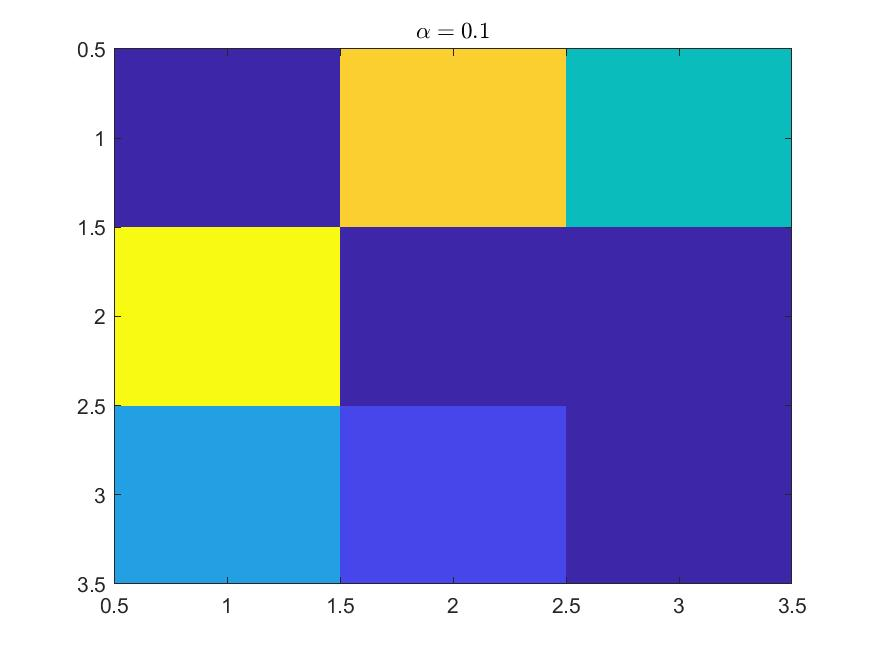
\includegraphics[width=.18\textwidth]{alpha1n3.jpg} & 
		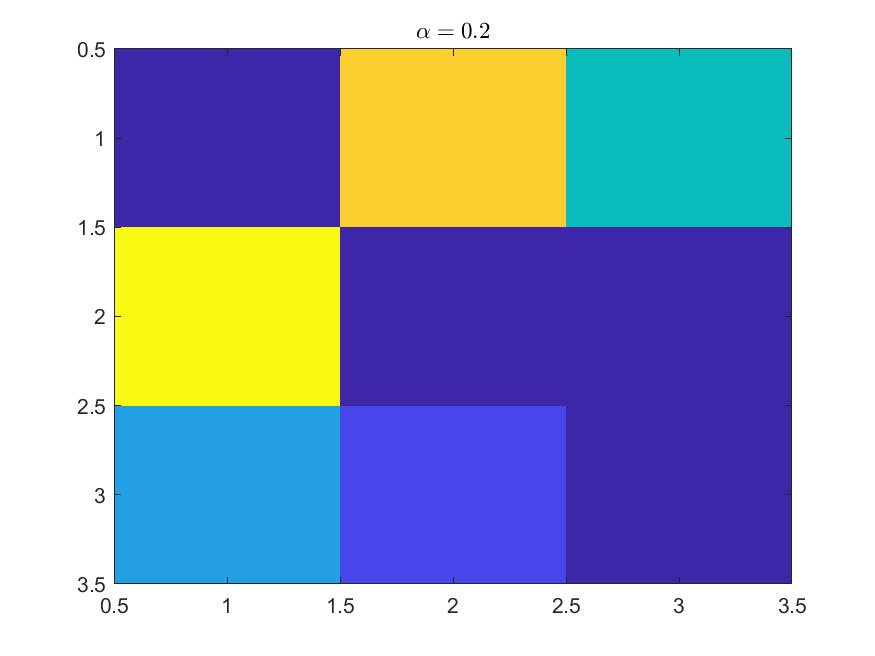
\includegraphics[width=.18\textwidth]{alpha2n3.jpg} & 
		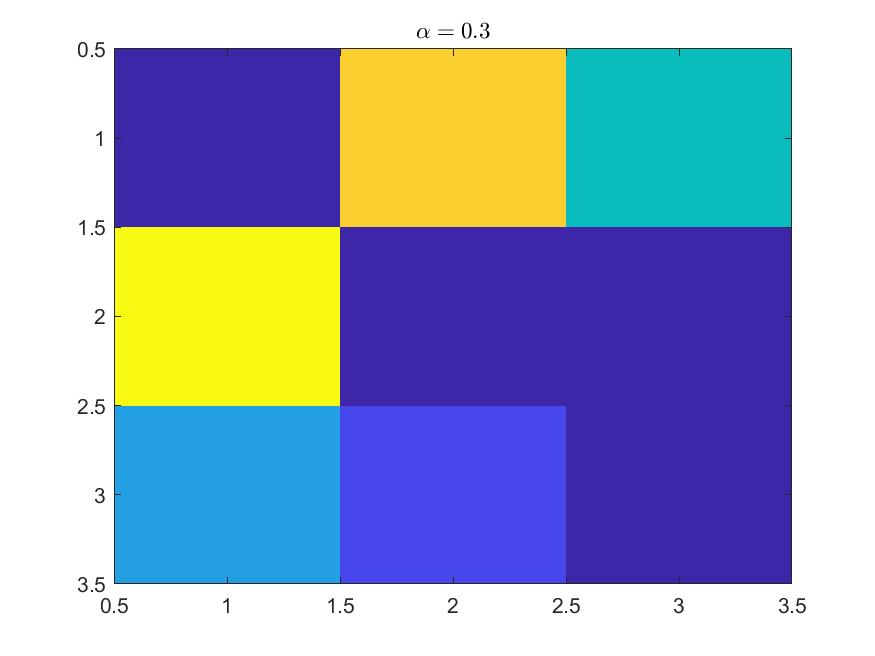
\includegraphics[width=.18\textwidth]{alpha3n3.jpg} & 
		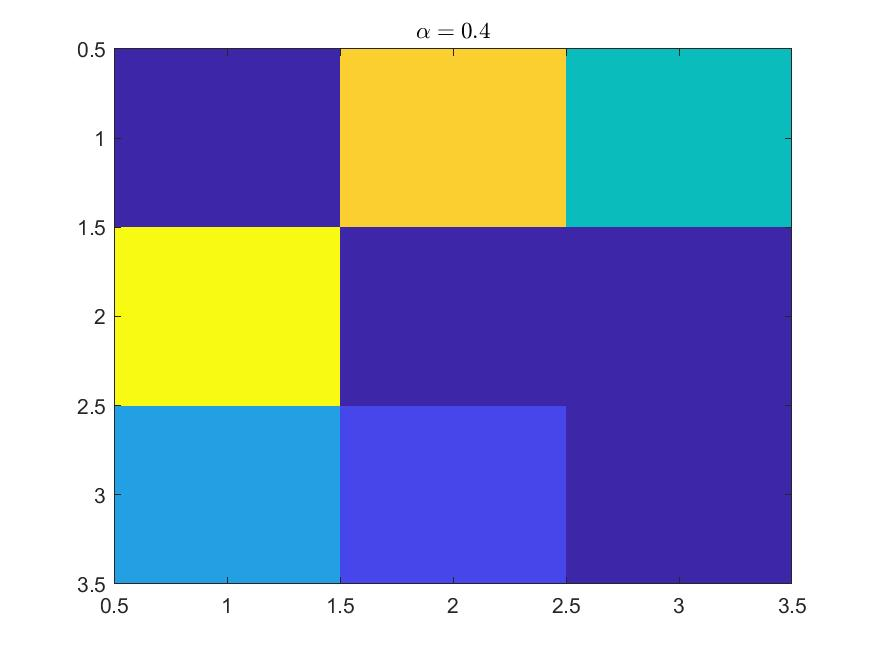
\includegraphics[width=.18\textwidth]{alpha4n3.jpg} & 
		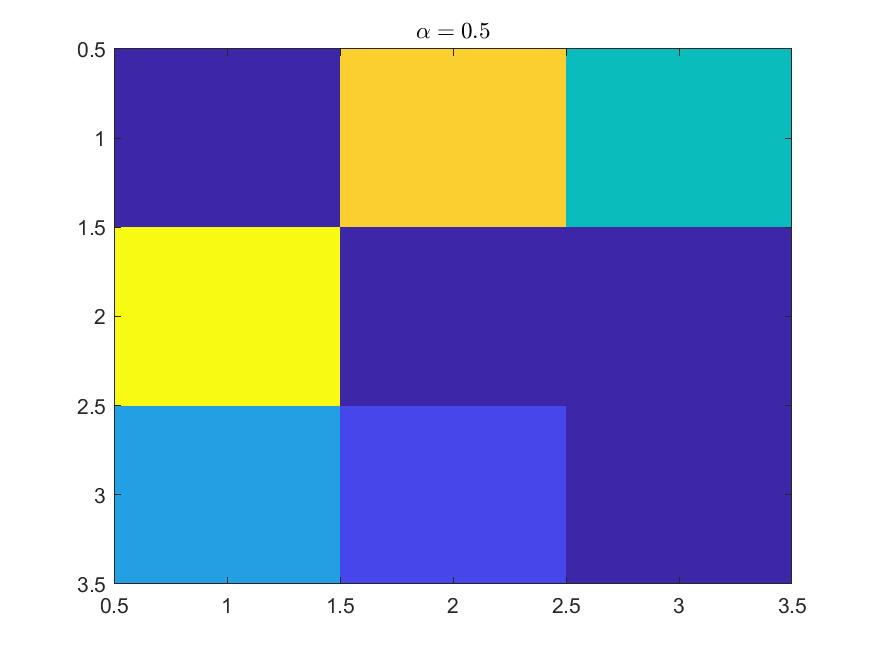
\includegraphics[width=.18\textwidth]{alpha5n3.jpg}\\
		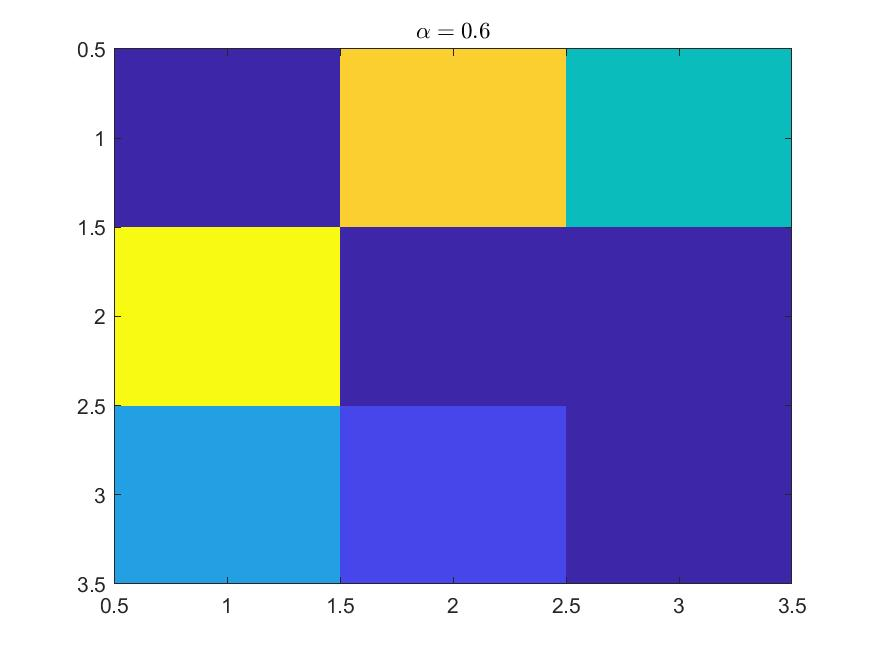
\includegraphics[width=.18\textwidth]{alpha6n3.jpg} & 
		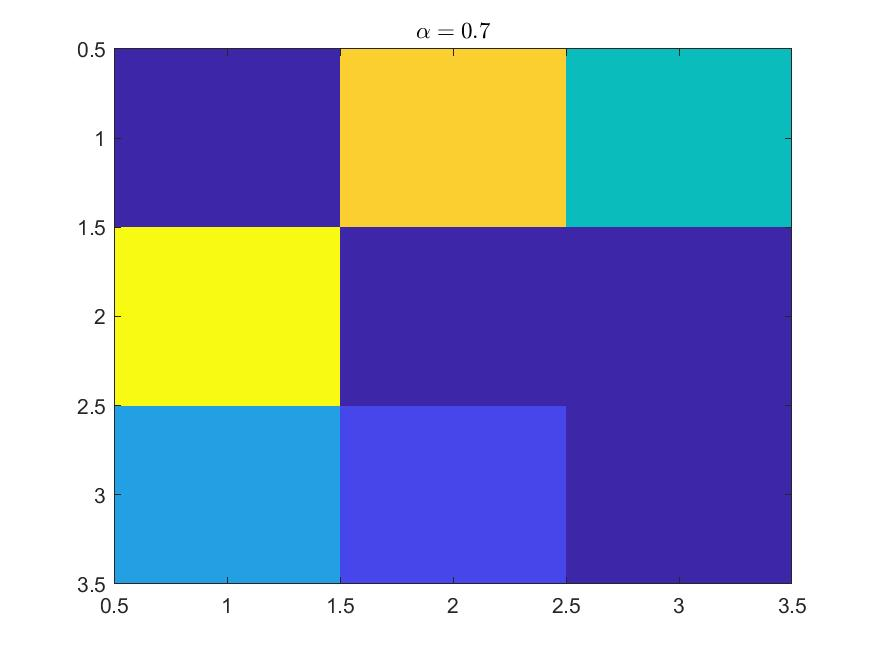
\includegraphics[width=.18\textwidth]{alpha7n3.jpg} &
		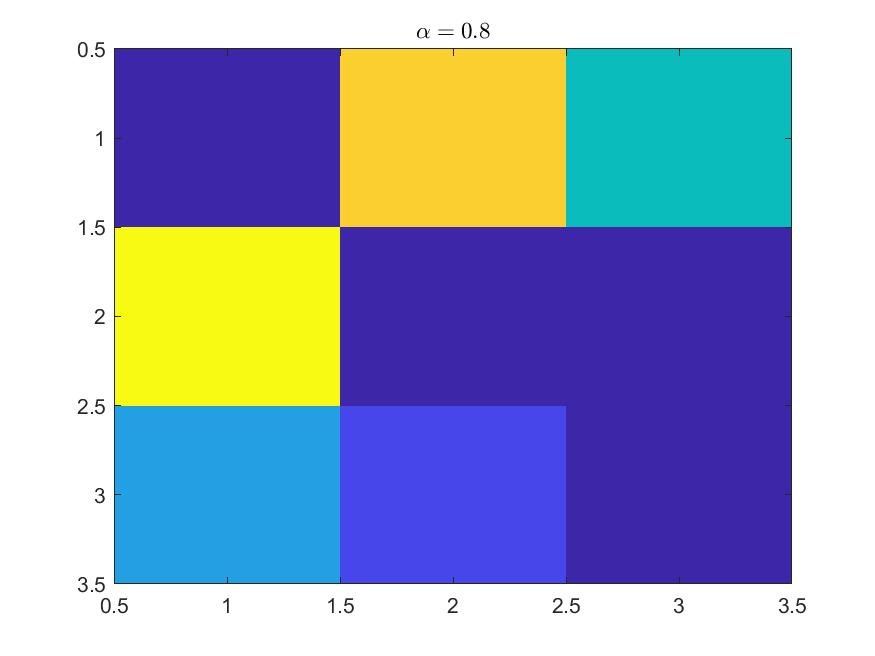
\includegraphics[width=.18\textwidth]{alpha8n3.jpg} & 
		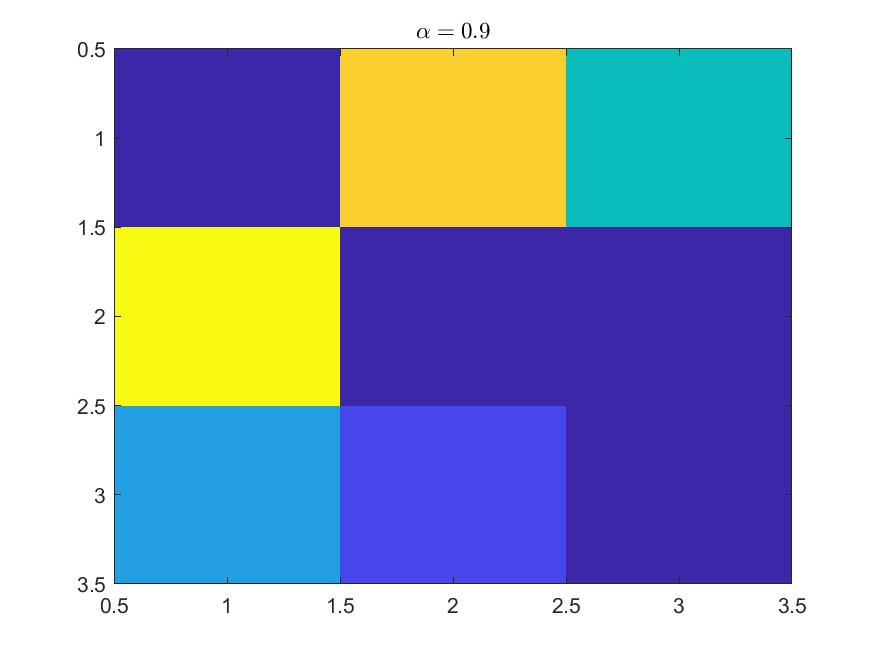
\includegraphics[width=.18\textwidth]{alpha9n3.jpg} & 
		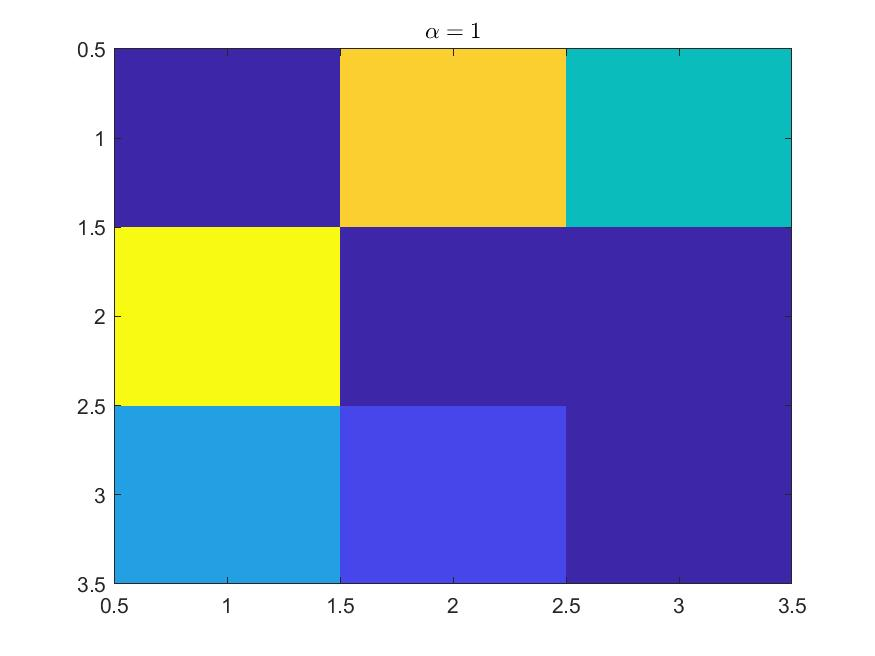
\includegraphics[width=.18\textwidth]{alpha10n3.jpg}
	\end{tabular}
	\caption{$n=3$, 不同松弛因子}
	\label{alphan3figure}
\end{figure}

\begin{figure}[htbp]
	\renewcommand{\captionfont}{\small}
	\centering
	\begin{tabular}{@{}ccccc@{}}
		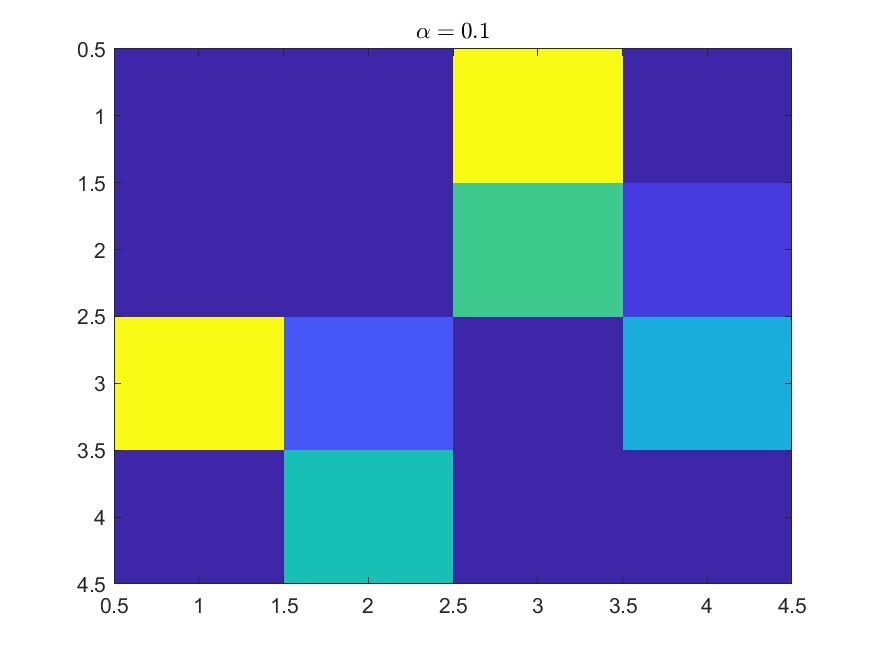
\includegraphics[width=.18\textwidth]{alpha1n4.jpg} & 
		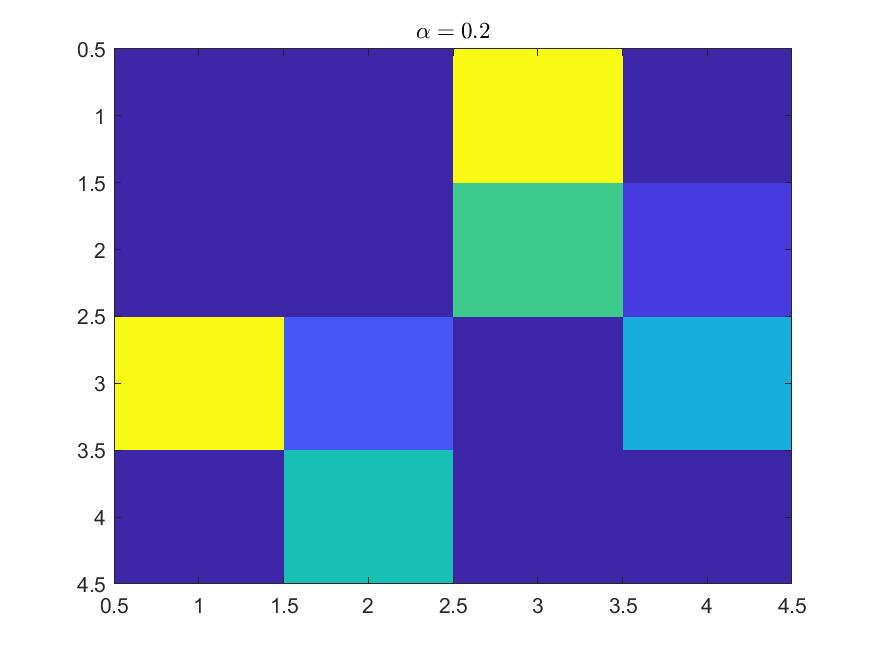
\includegraphics[width=.18\textwidth]{alpha2n4.jpg} & 
		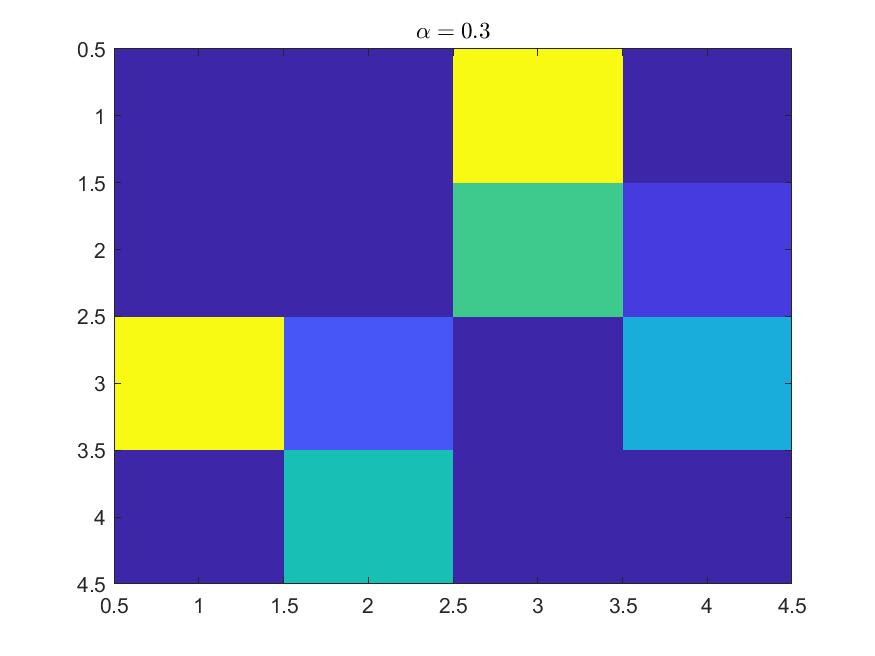
\includegraphics[width=.18\textwidth]{alpha3n4.jpg} & 
		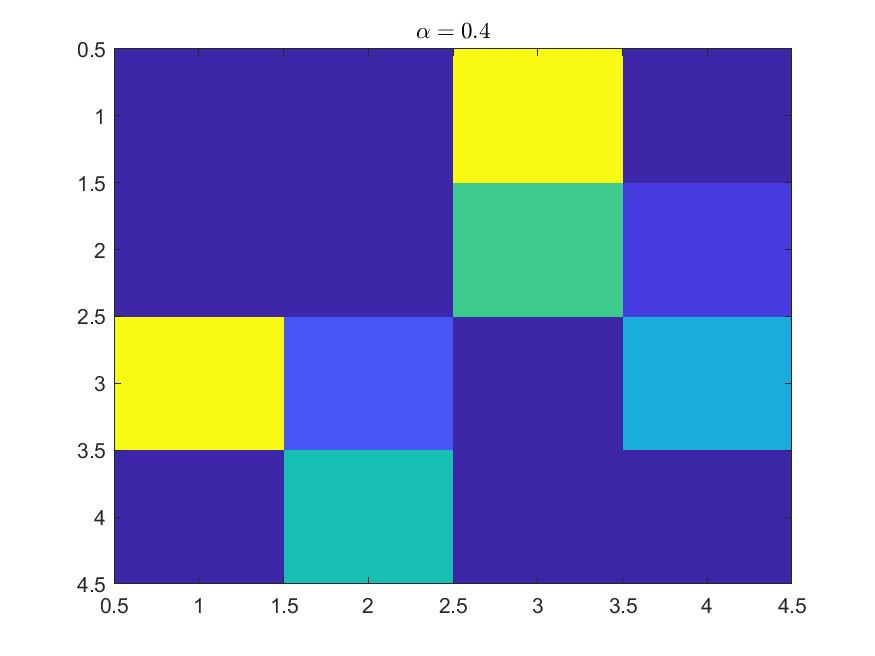
\includegraphics[width=.18\textwidth]{alpha4n4.jpg} & 
		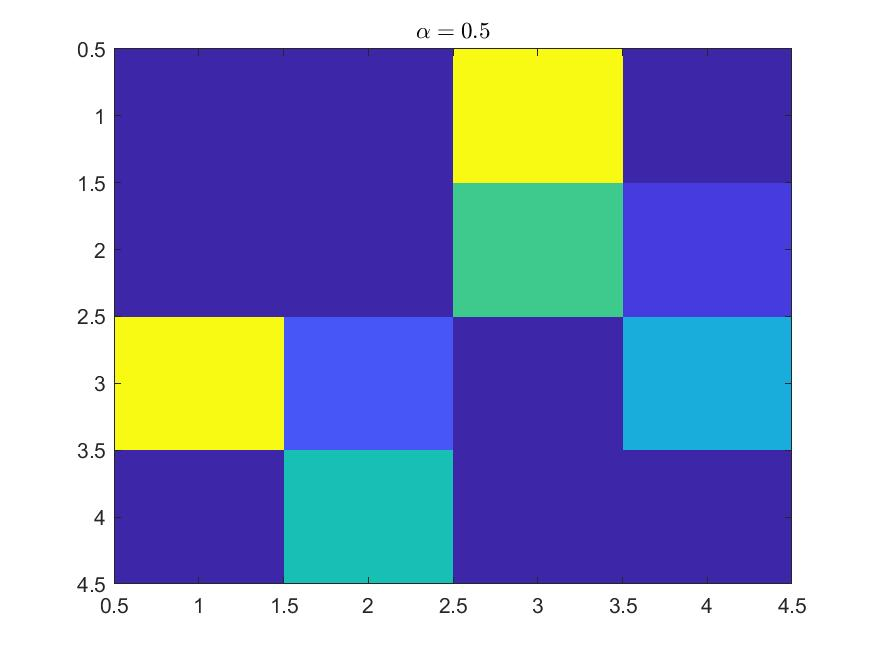
\includegraphics[width=.18\textwidth]{alpha5n4.jpg}\\
		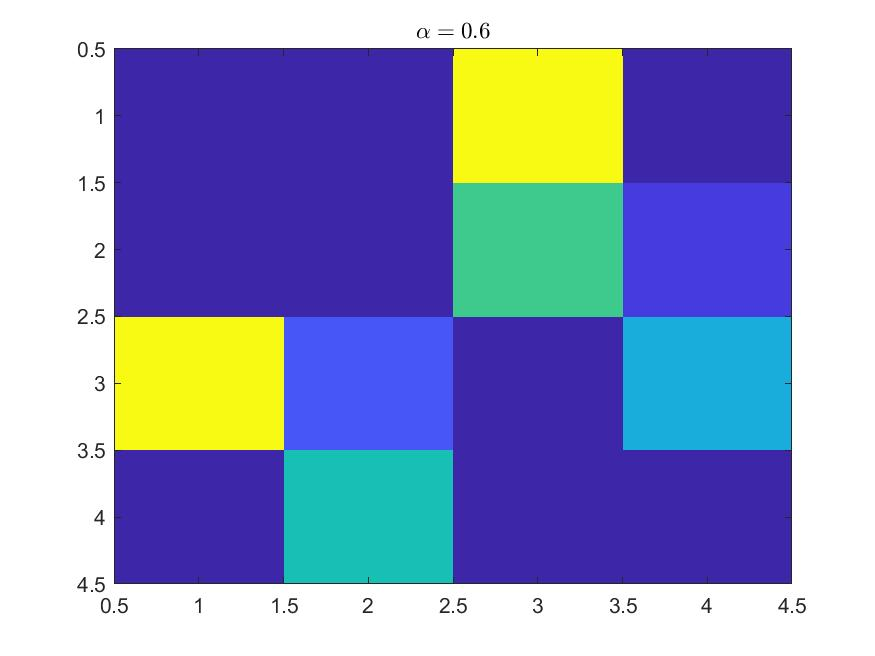
\includegraphics[width=.18\textwidth]{alpha6n4.jpg} & 
		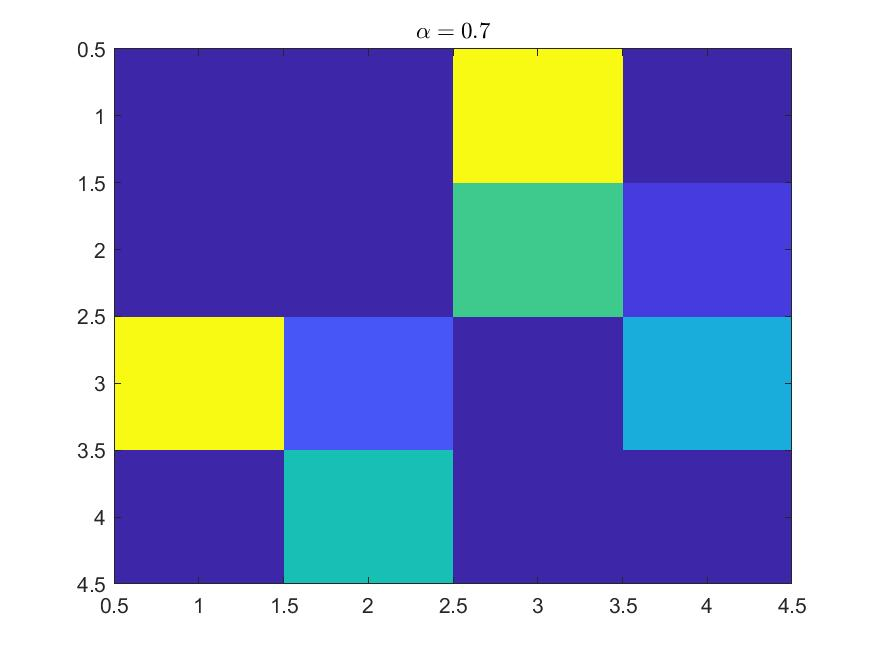
\includegraphics[width=.18\textwidth]{alpha7n4.jpg} &
		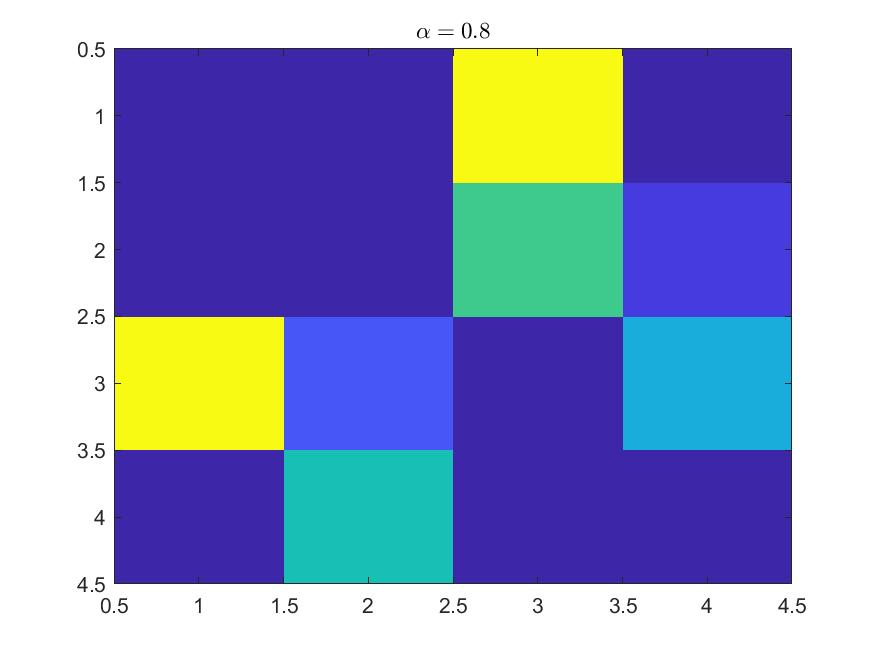
\includegraphics[width=.18\textwidth]{alpha8n4.jpg} & 
		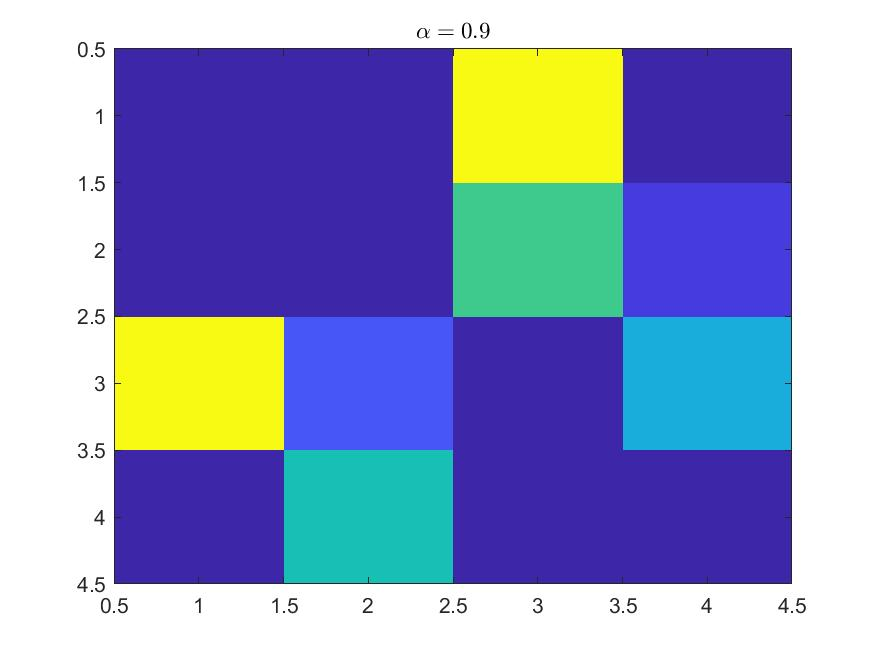
\includegraphics[width=.18\textwidth]{alpha9n4.jpg} & 
		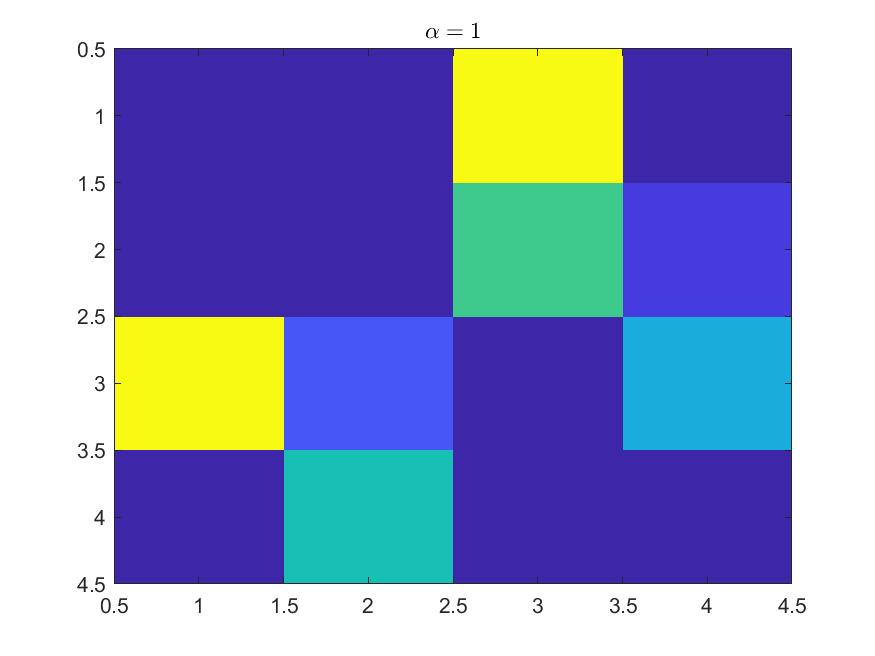
\includegraphics[width=.18\textwidth]{alpha10n4.jpg}
	\end{tabular}
	\caption{$n=4$, 不同松弛因子}
	\label{alphan4figure}
\end{figure}

\begin{figure}[htbp]
	\renewcommand{\captionfont}{\small}
	\centering
	\begin{tabular}{@{}ccccc@{}}
		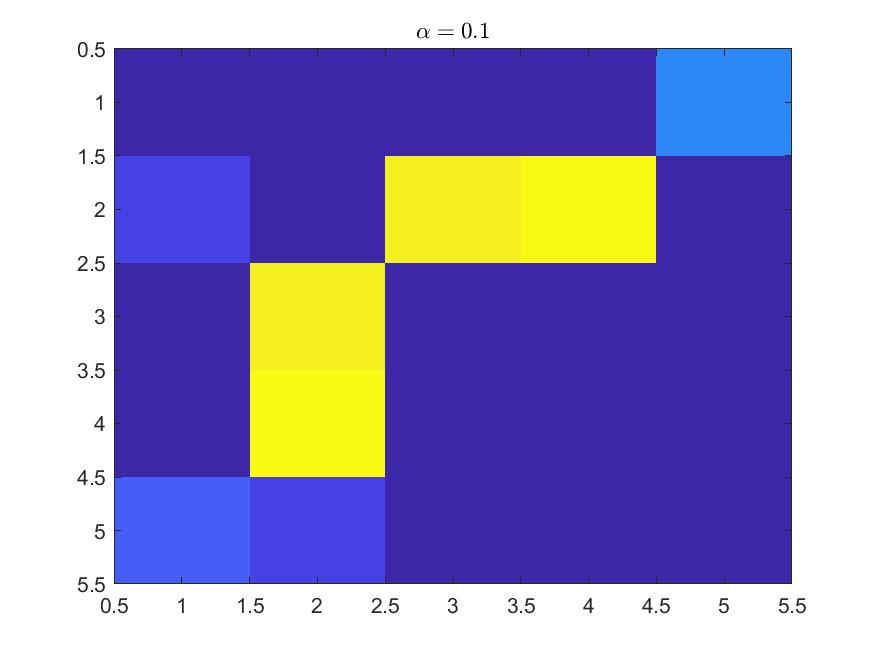
\includegraphics[width=.18\textwidth]{alpha1n5.jpg} & 
		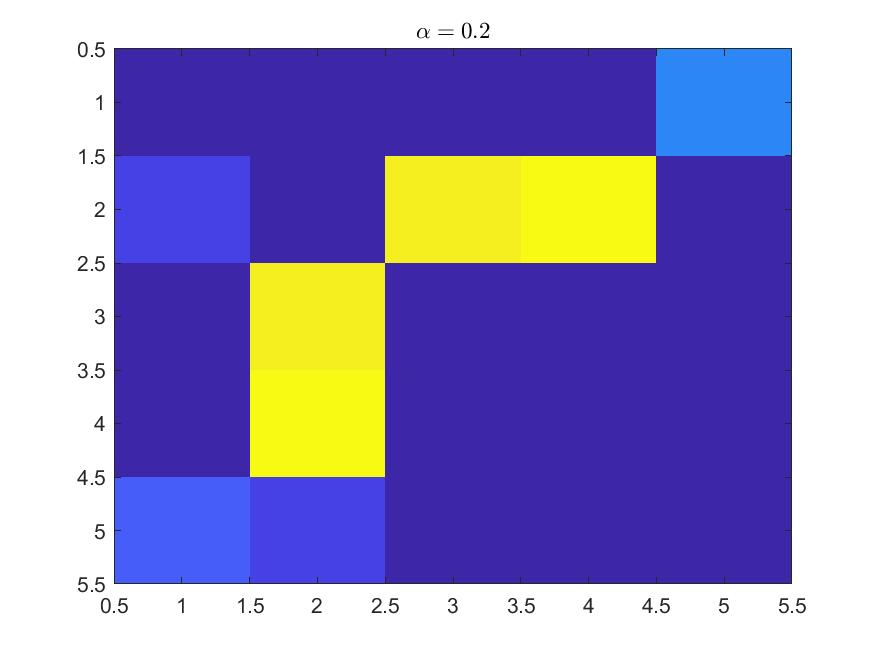
\includegraphics[width=.18\textwidth]{alpha2n5.jpg} & 
		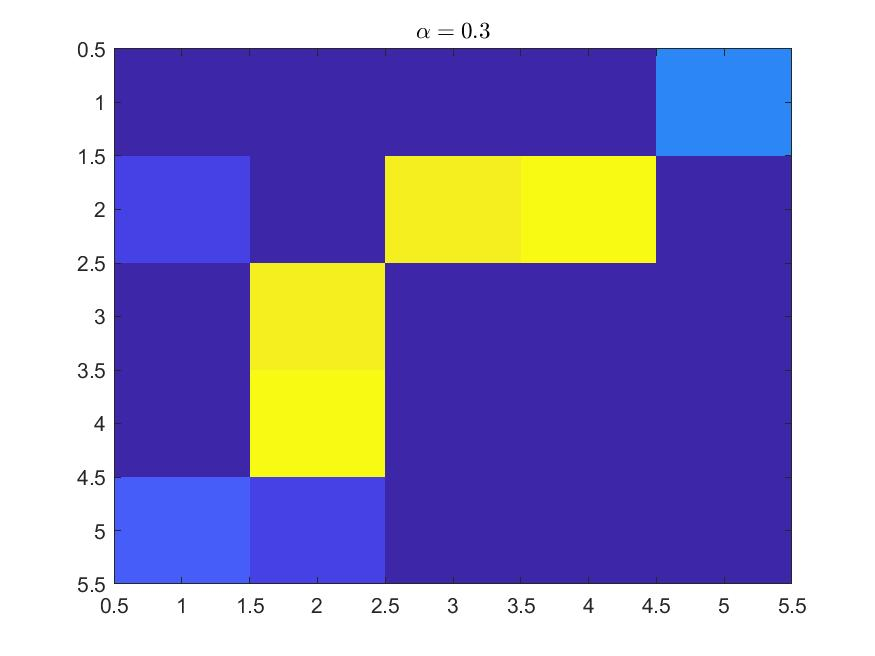
\includegraphics[width=.18\textwidth]{alpha3n5.jpg} & 
		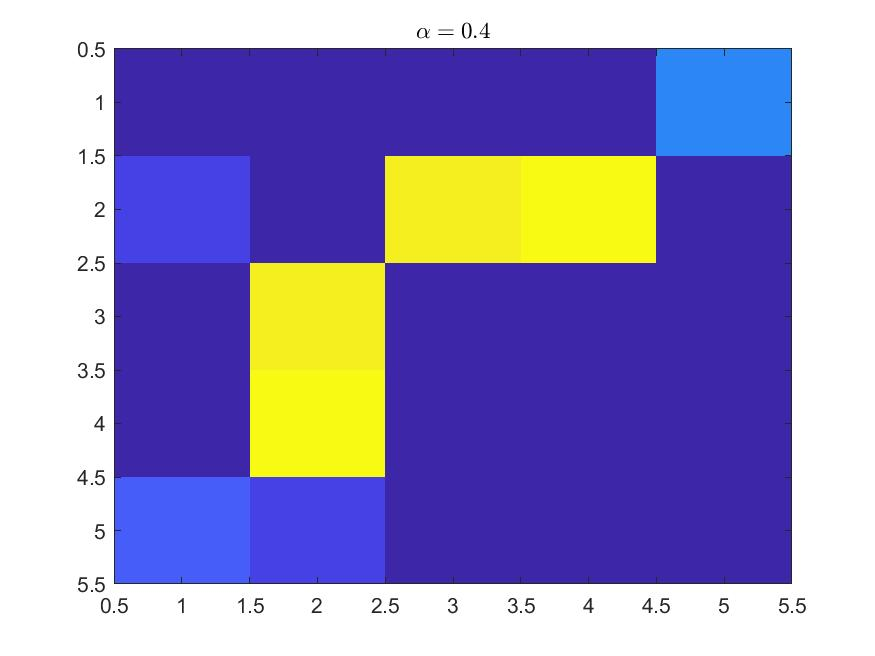
\includegraphics[width=.18\textwidth]{alpha4n5.jpg} & 
		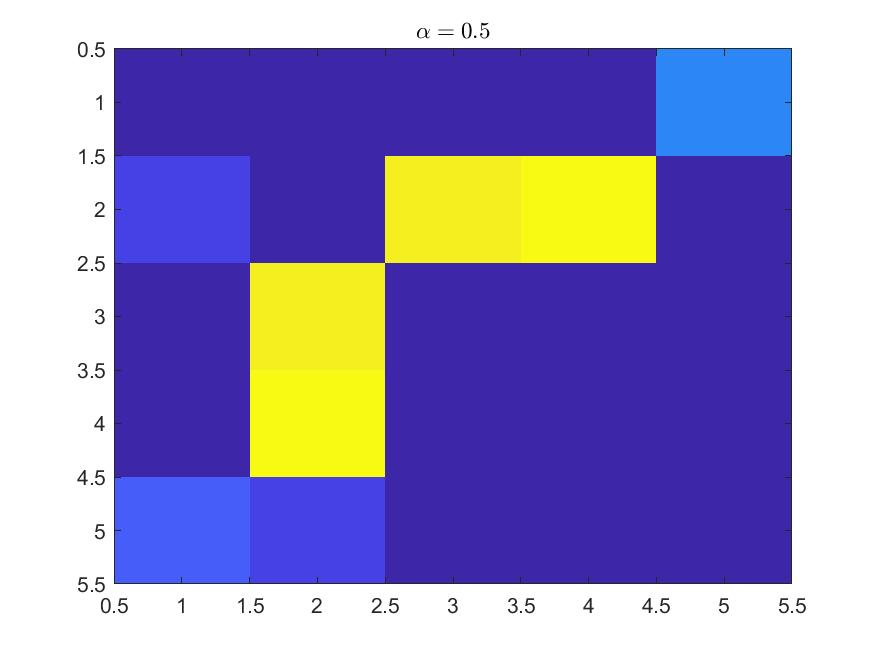
\includegraphics[width=.18\textwidth]{alpha5n5.jpg}\\
		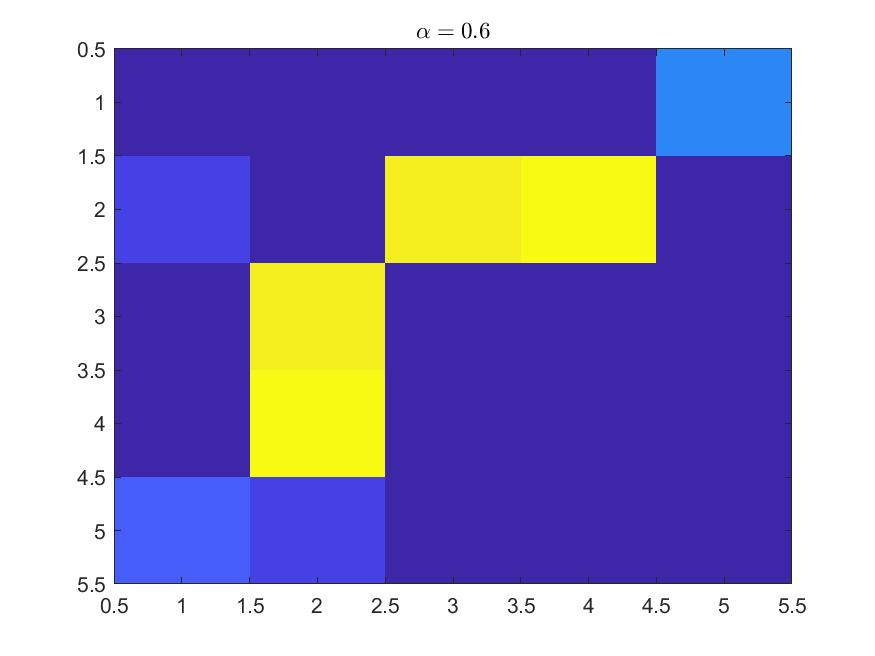
\includegraphics[width=.18\textwidth]{alpha6n5.jpg} & 
		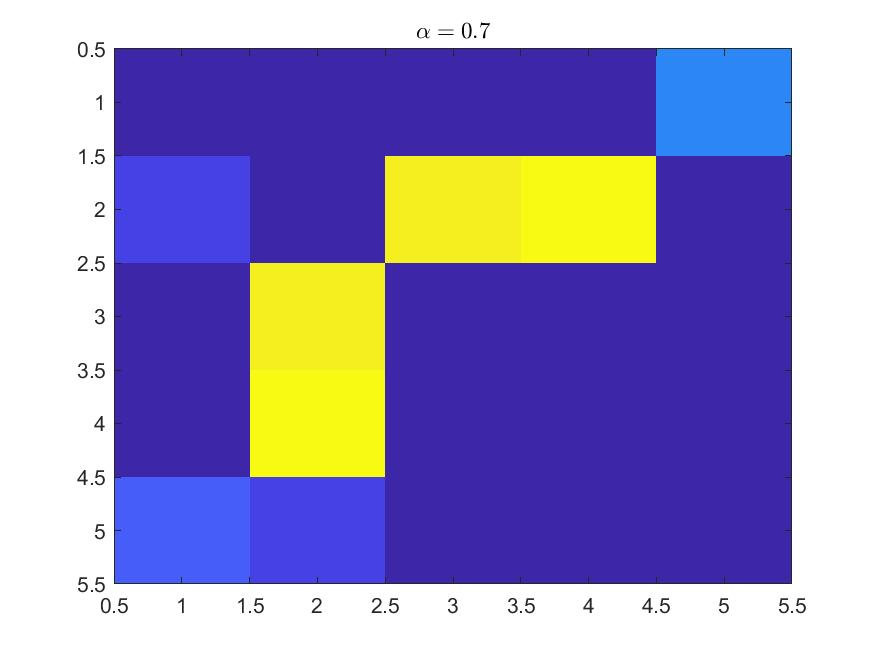
\includegraphics[width=.18\textwidth]{alpha7n5.jpg} &
		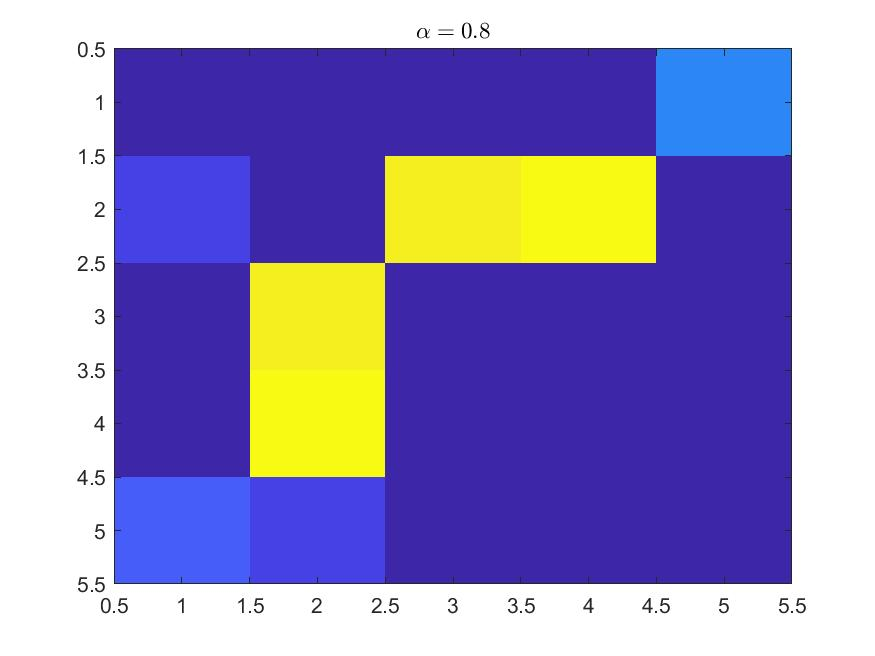
\includegraphics[width=.18\textwidth]{alpha8n5.jpg} & 
		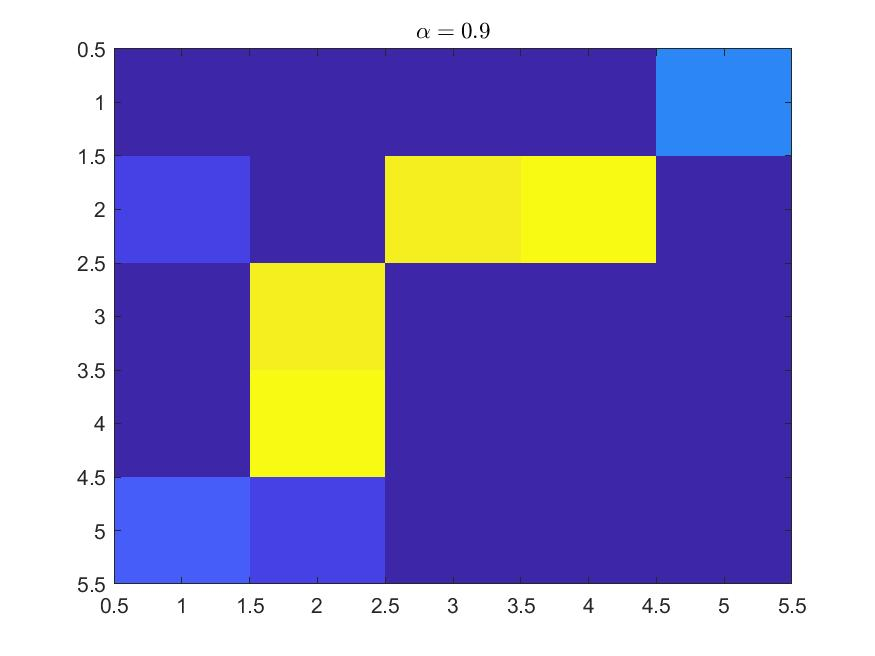
\includegraphics[width=.18\textwidth]{alpha9n5.jpg} & 
		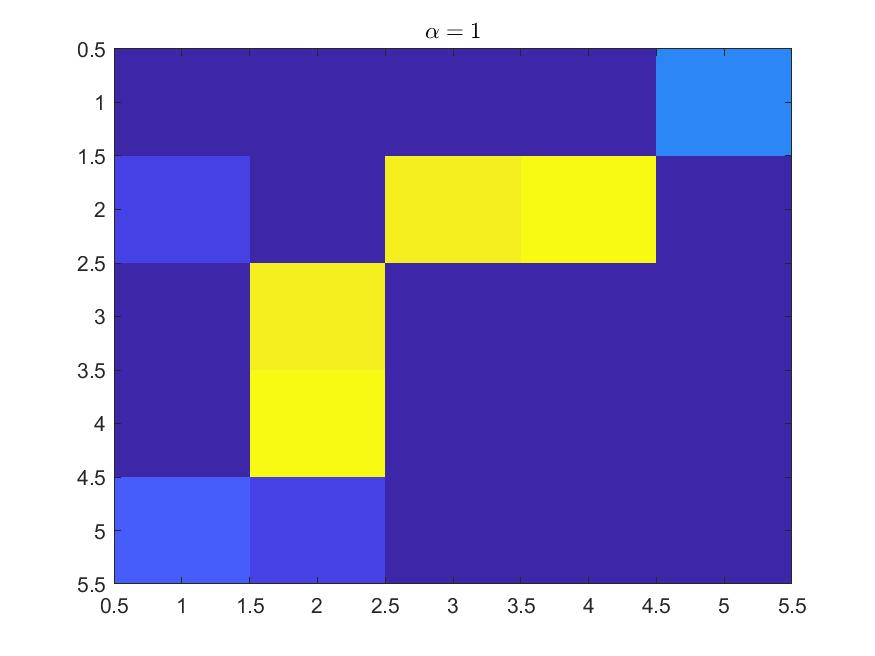
\includegraphics[width=.18\textwidth]{alpha10n5.jpg}
	\end{tabular}
	\caption{$n=5$, 不同松弛因子}
	\label{alphan5figure}
\end{figure}

\begin{figure}[htbp]
	\renewcommand{\captionfont}{\small}
	\centering
	\begin{tabular}{@{}ccccc@{}}
		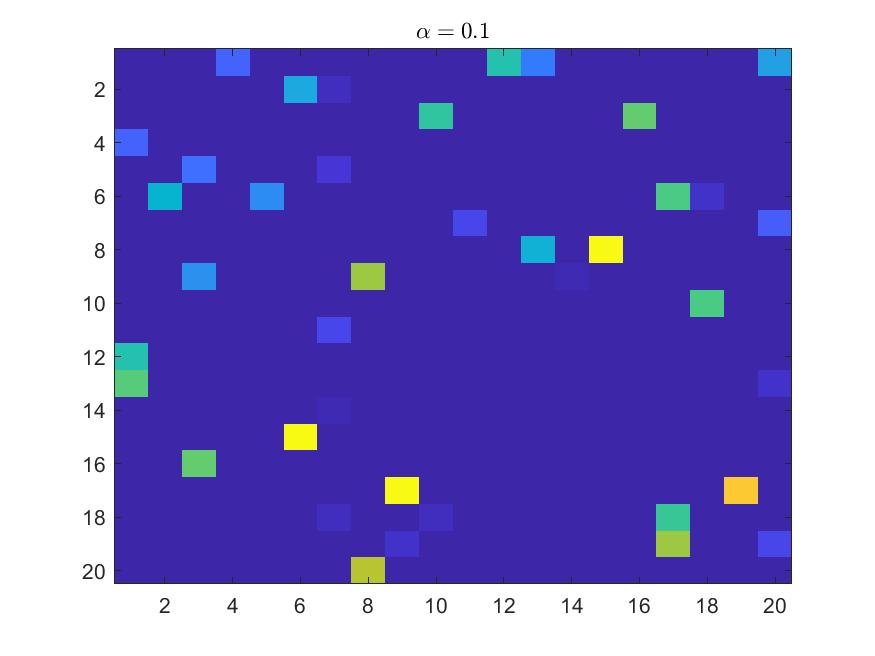
\includegraphics[width=.18\textwidth]{alpha1n20.jpg} & 
		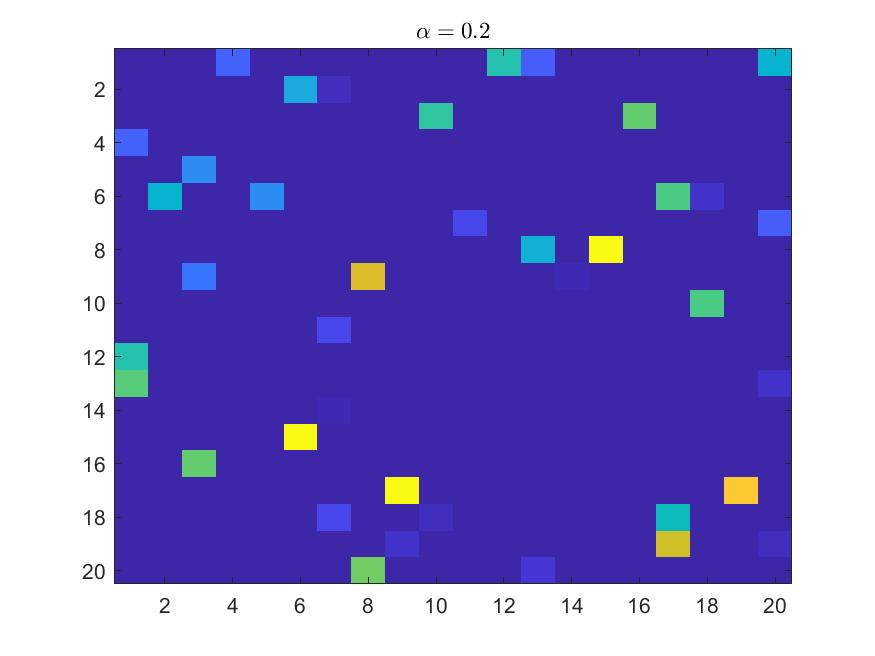
\includegraphics[width=.18\textwidth]{alpha2n20.jpg} & 
		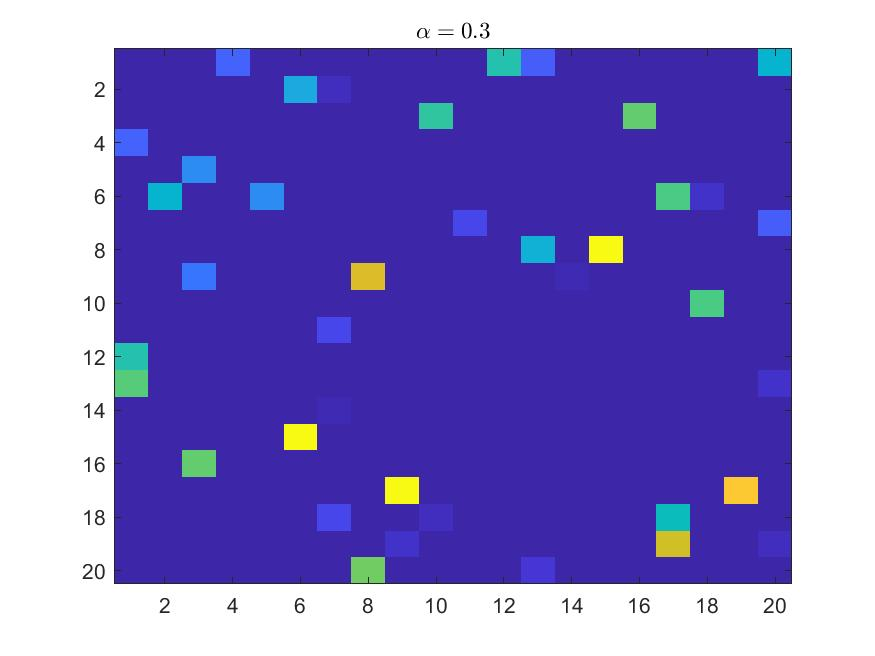
\includegraphics[width=.18\textwidth]{alpha3n20.jpg} & 
		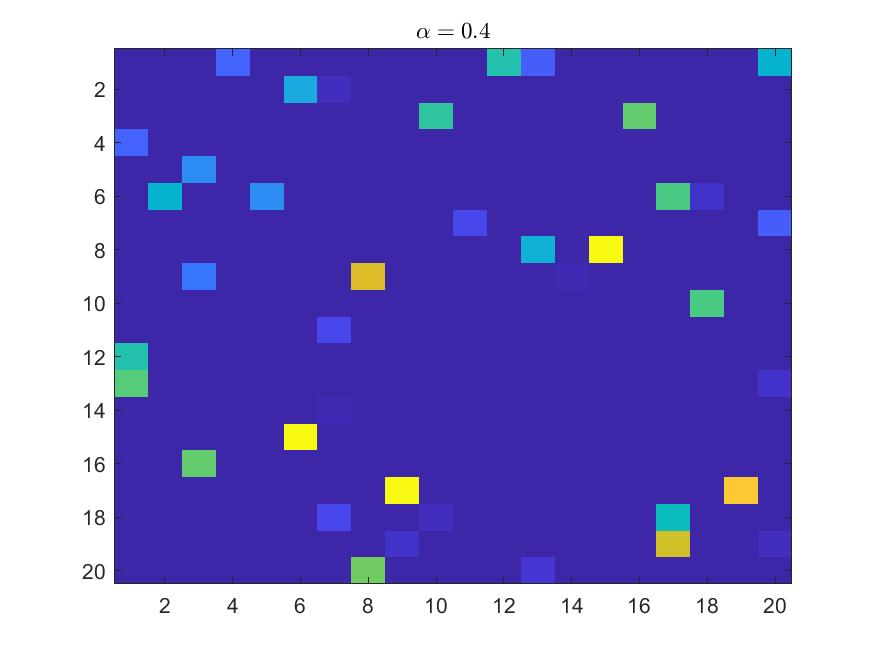
\includegraphics[width=.18\textwidth]{alpha4n20.jpg} & 
		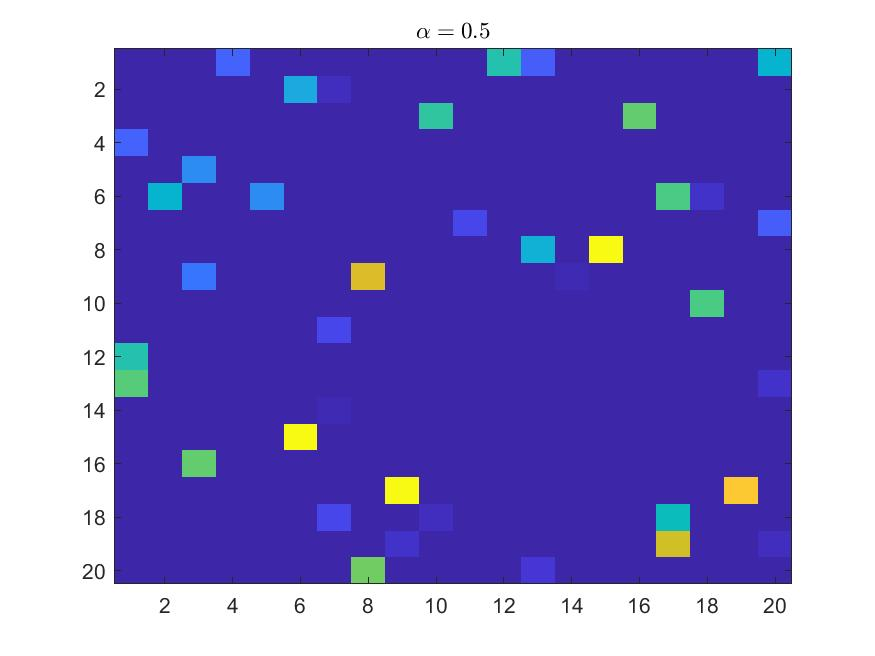
\includegraphics[width=.18\textwidth]{alpha5n20.jpg}\\
		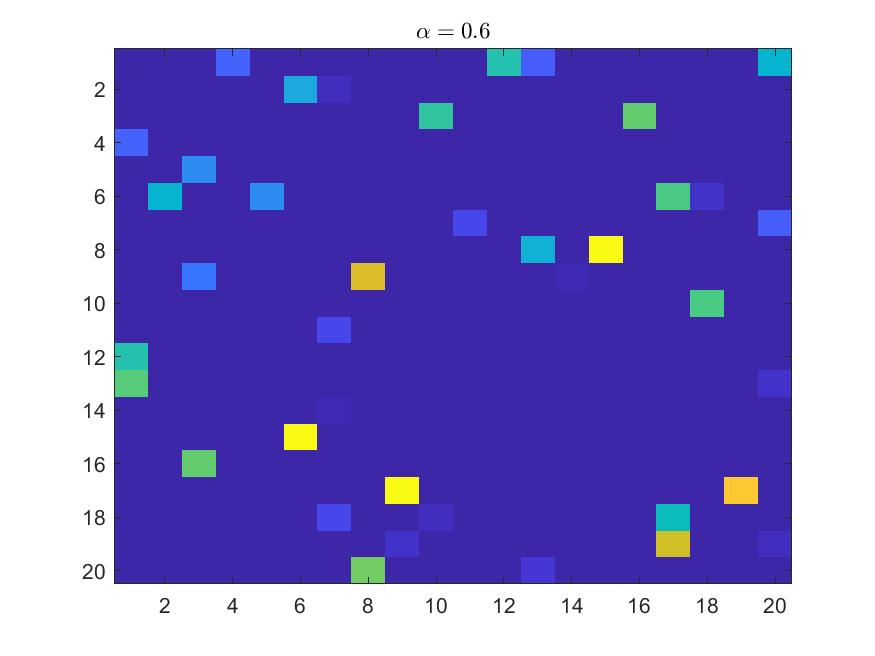
\includegraphics[width=.18\textwidth]{alpha6n20.jpg} & 
		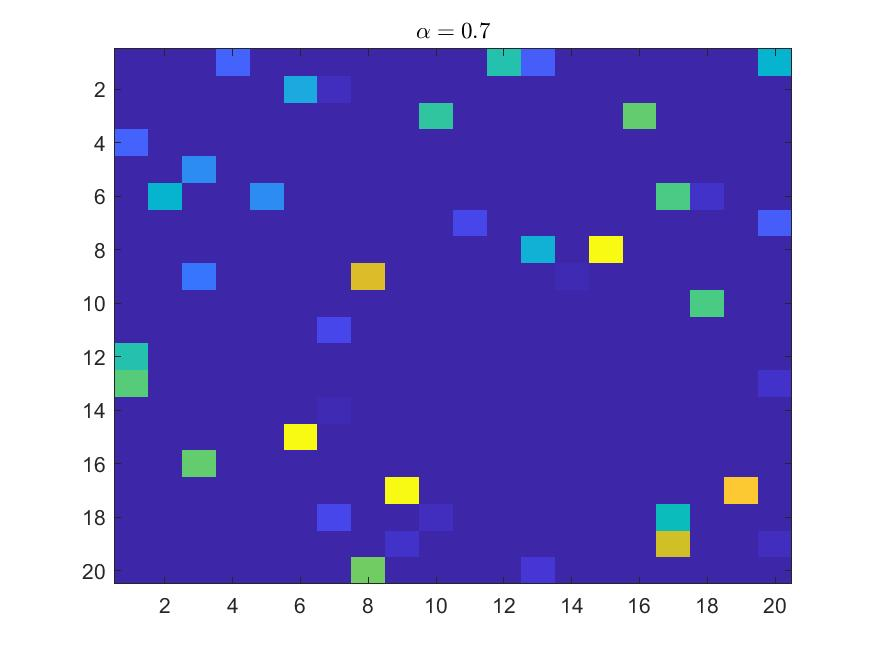
\includegraphics[width=.18\textwidth]{alpha7n20.jpg} &
		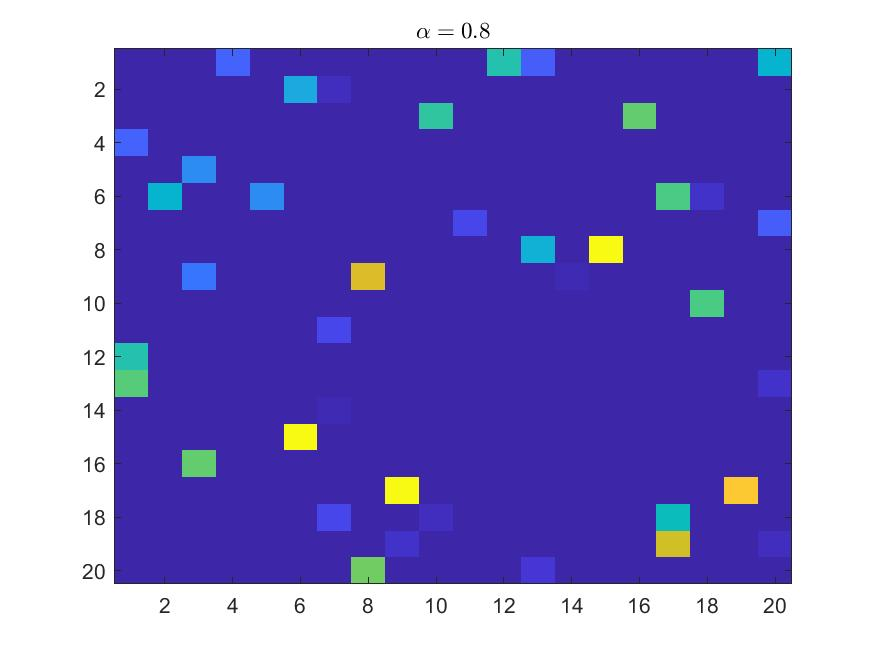
\includegraphics[width=.18\textwidth]{alpha8n20.jpg} & 
		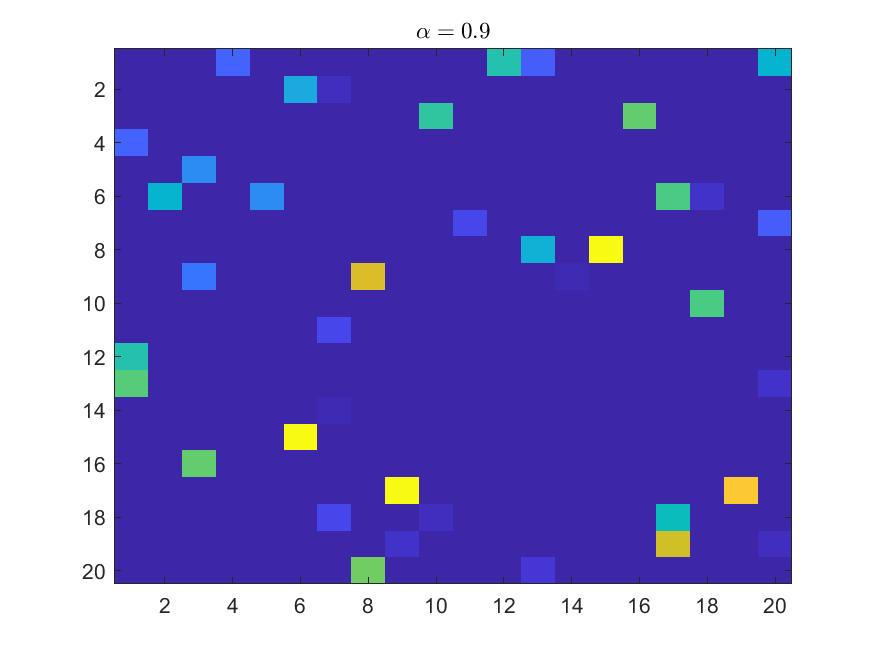
\includegraphics[width=.18\textwidth]{alpha9n20.jpg} & 
		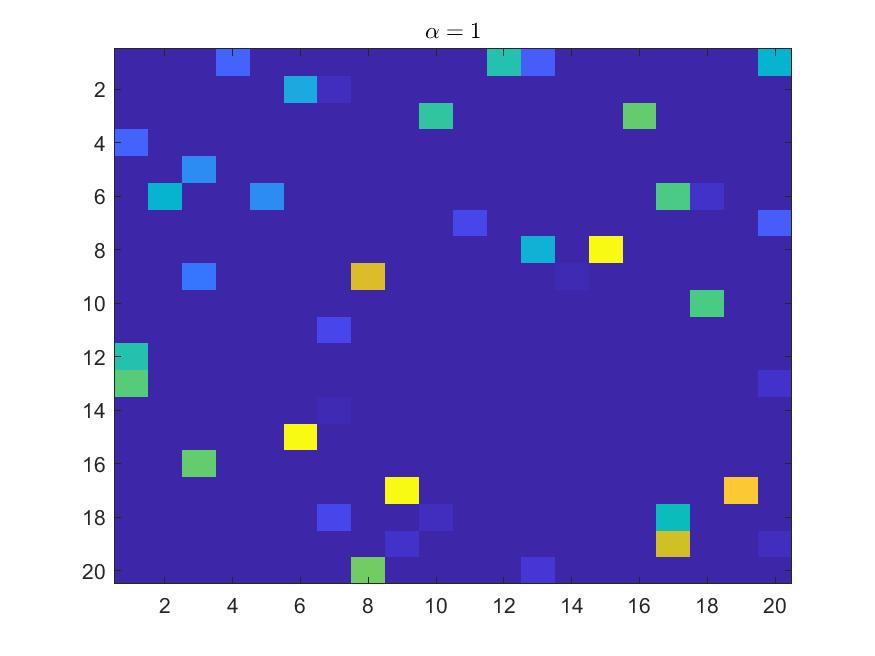
\includegraphics[width=.18\textwidth]{alpha10n20.jpg}
	\end{tabular}
	\caption{$n=20$, 不同松弛因子}
	\label{alphan20figure}
\end{figure}

\begin{figure}[htbp]
	\renewcommand{\captionfont}{\small}
	\centering
	\begin{tabular}{@{}ccccc@{}}
		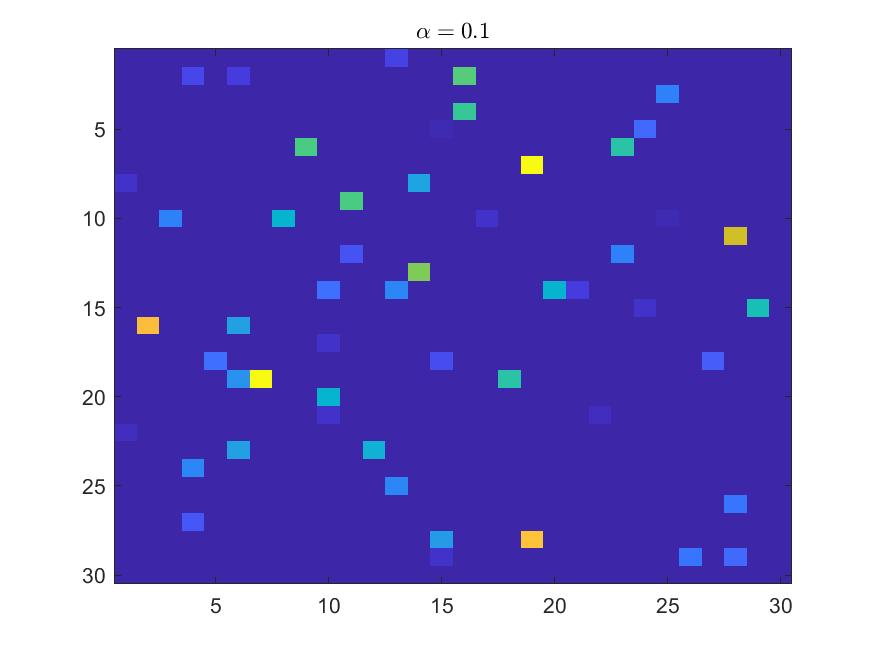
\includegraphics[width=.18\textwidth]{alpha1n30.jpg} & 
		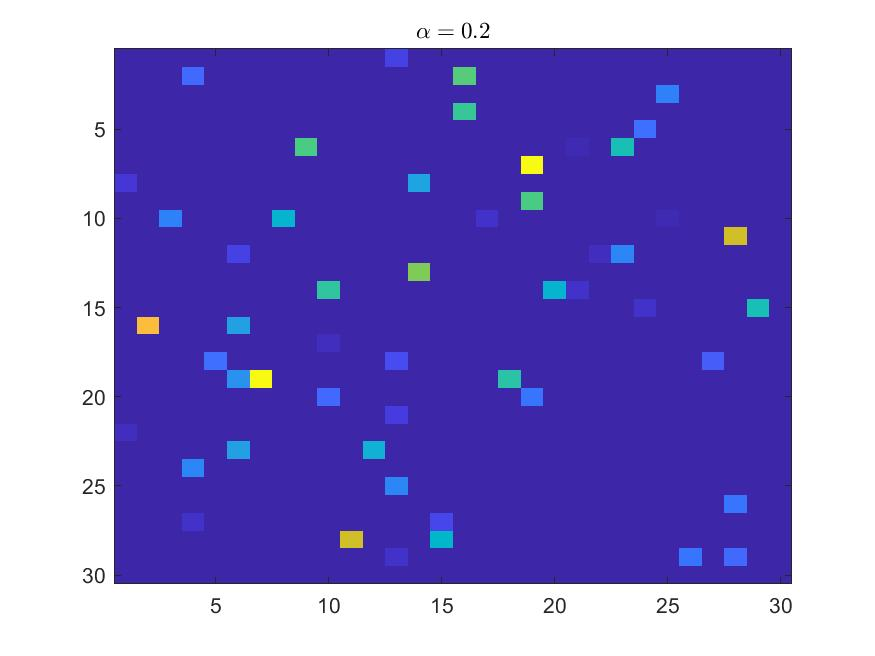
\includegraphics[width=.18\textwidth]{alpha2n30.jpg} & 
		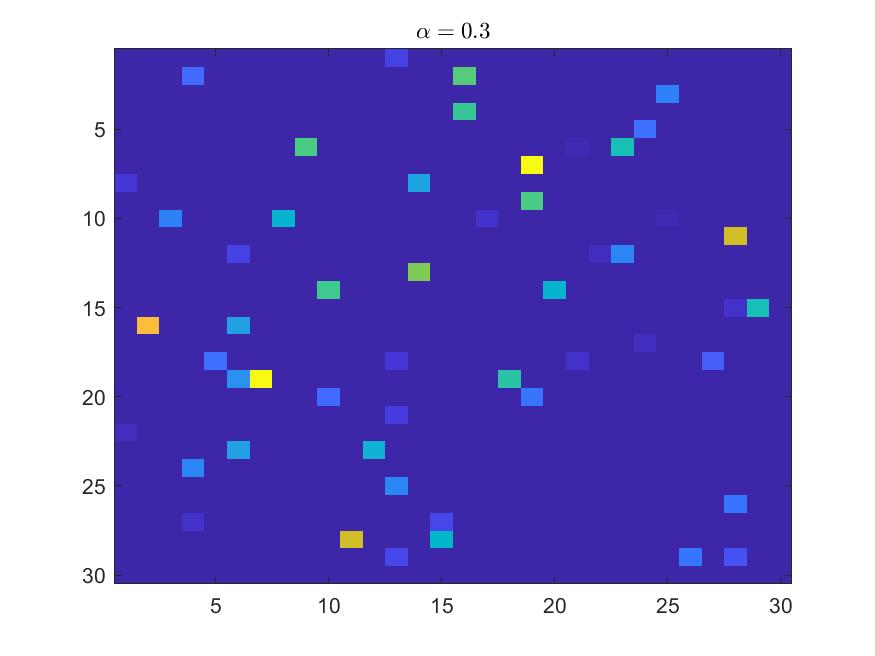
\includegraphics[width=.18\textwidth]{alpha3n30.jpg} & 
		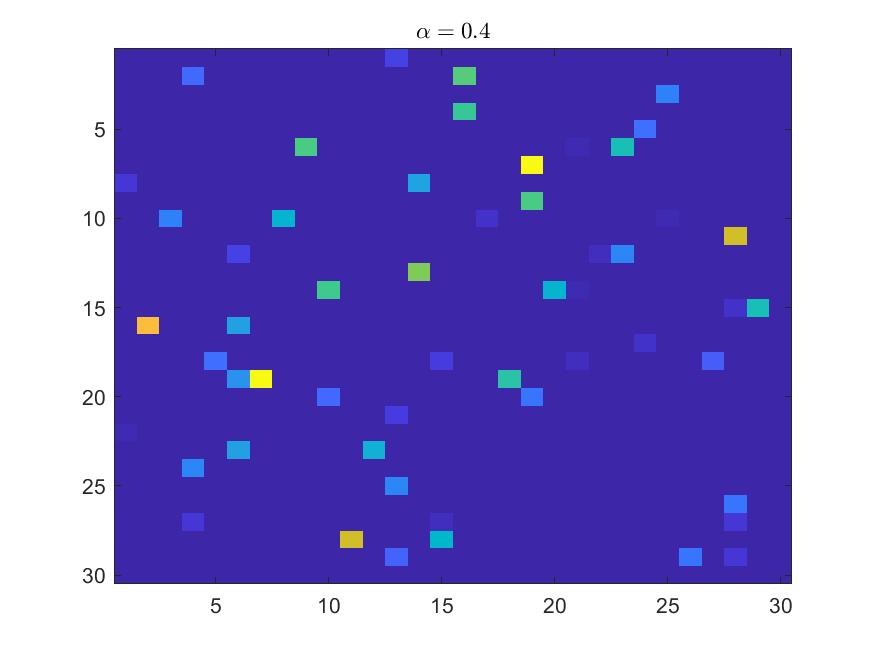
\includegraphics[width=.18\textwidth]{alpha4n30.jpg} & 
		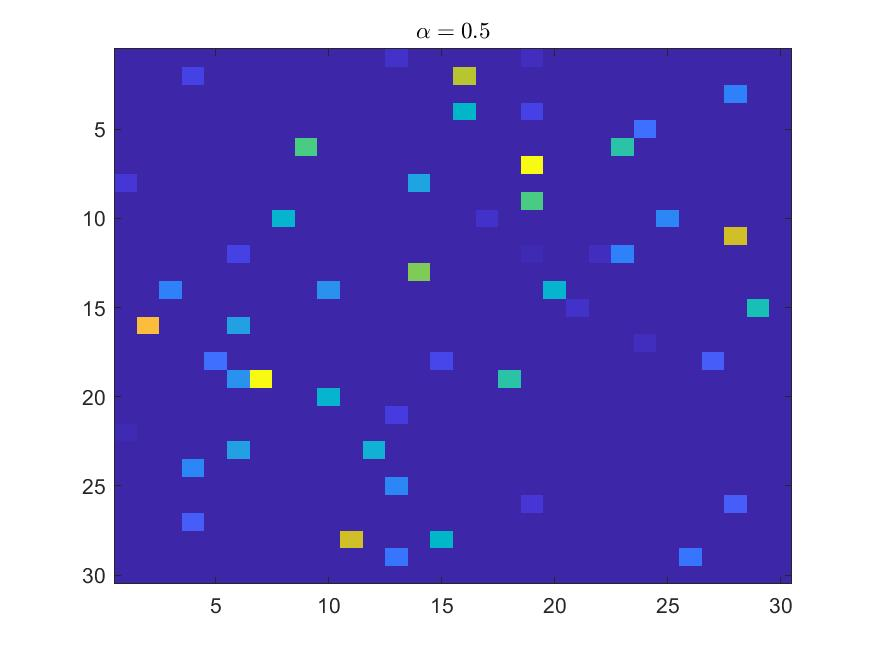
\includegraphics[width=.18\textwidth]{alpha5n30.jpg}\\
		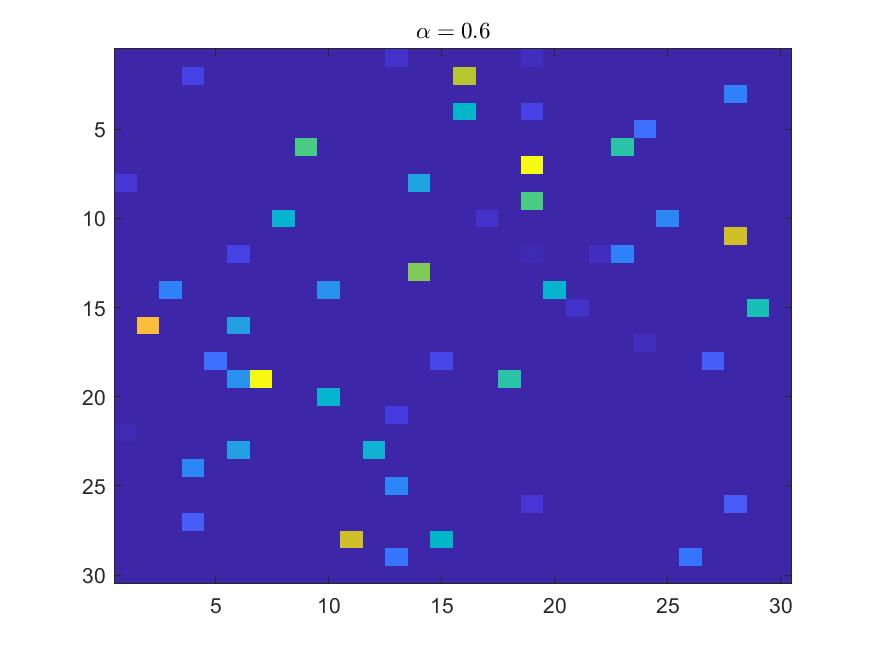
\includegraphics[width=.18\textwidth]{alpha6n30.jpg} & 
		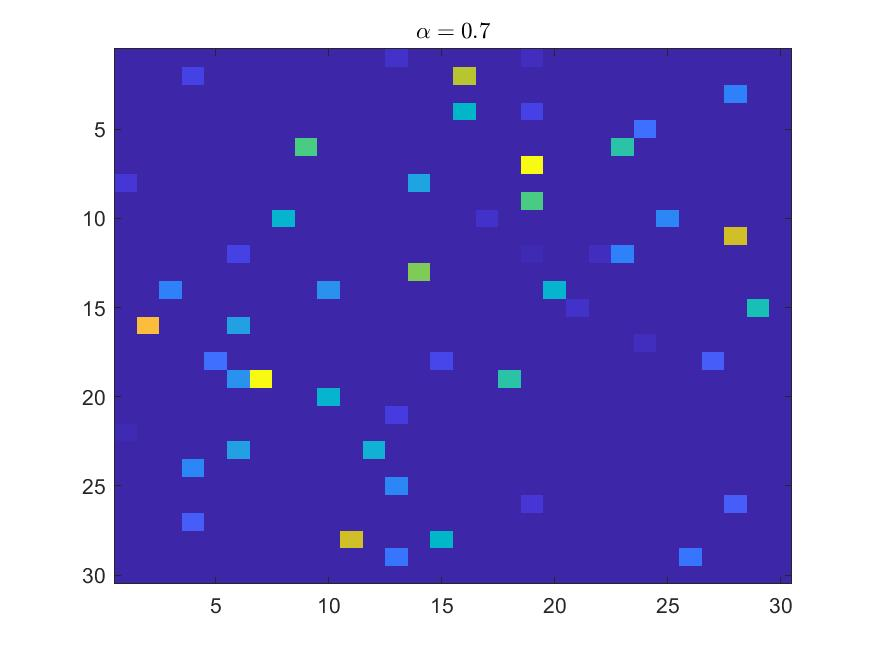
\includegraphics[width=.18\textwidth]{alpha7n30.jpg} &
		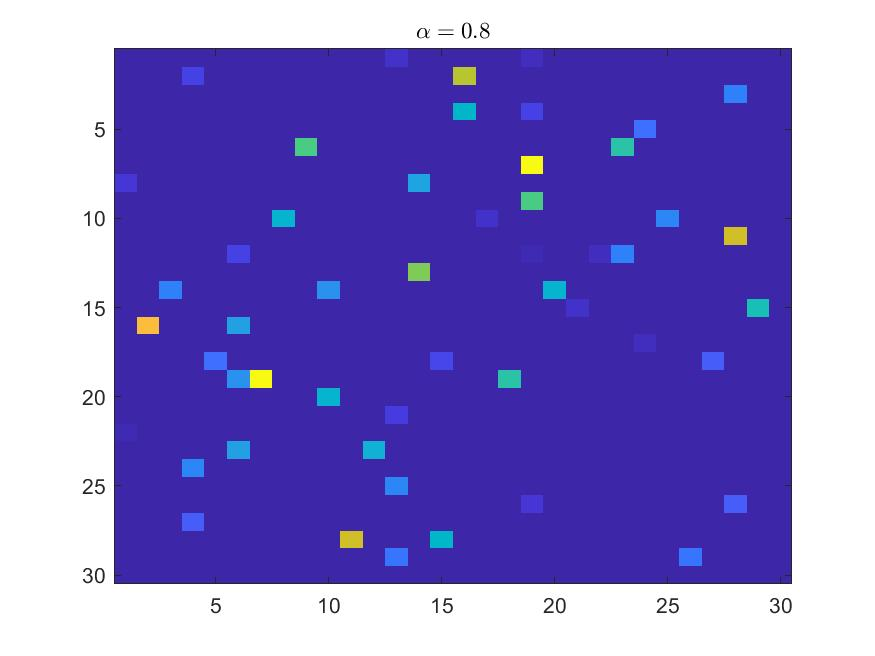
\includegraphics[width=.18\textwidth]{alpha8n30.jpg} & 
		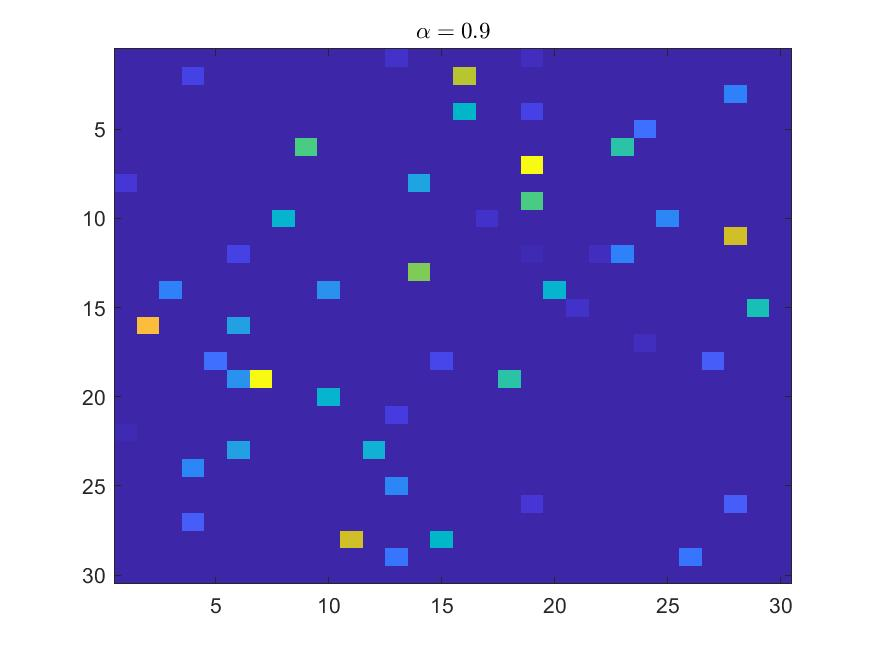
\includegraphics[width=.18\textwidth]{alpha9n30.jpg} & 
		\includegraphics[width=.18\textwidth]{alpha10n30.jpg}
	\end{tabular}
	\caption{$n=30$, 不同松弛因子}
	\label{alphan30figure}
\end{figure}

\begin{figure}[htbp]
	\renewcommand{\captionfont}{\small}
	\centering
	\begin{tabular}{@{}ccccc@{}}
		\includegraphics[width=.18\textwidth]{alpha1n40.jpg} & 
		\includegraphics[width=.18\textwidth]{alpha2n40.jpg} & 
		\includegraphics[width=.18\textwidth]{alpha3n40.jpg} & 
		\includegraphics[width=.18\textwidth]{alpha4n40.jpg} & 
		\includegraphics[width=.18\textwidth]{alpha5n40.jpg}\\
		\includegraphics[width=.18\textwidth]{alpha6n40.jpg} & 
		\includegraphics[width=.18\textwidth]{alpha7n40.jpg} &
		\includegraphics[width=.18\textwidth]{alpha8n40.jpg} & 
		\includegraphics[width=.18\textwidth]{alpha9n40.jpg} & 
		\includegraphics[width=.18\textwidth]{alpha10n40.jpg}
	\end{tabular}
	\caption{$n=40$, 不同松弛因子}
	\label{alphan40figure}
\end{figure}
图中不同颜色代表了不同的取值, 颜色相近代表取值相近.
\par 典型的收敛曲线如图\ref{converge curve}所示. 
\begin{figure}[htbp]
	\renewcommand{\captionfont}{\small}
	\centering
	\subfigure[$\alpha=0.1,n=3$]{
	\begin{minipage}[b]{.31\linewidth}
		\includegraphics[width=\linewidth]{n3primalres.jpg}\vspace{4pt}
		\includegraphics[width=\linewidth]{n3dualres.jpg}\vspace{4pt}
		\includegraphics[width=\linewidth]{n3obj.jpg}
	\end{minipage}
	}
	\subfigure[$\alpha=0.2,n=4$]{
		\begin{minipage}[b]{.31\linewidth}
			\includegraphics[width=\linewidth]{n4primalres.jpg}\vspace{4pt}
			\includegraphics[width=\linewidth]{n4dualres.jpg}\vspace{4pt}
			\includegraphics[width=\linewidth]{n4obj.jpg}
		\end{minipage}
		}
	\subfigure[$\alpha=0.8,n=5$]{
		\begin{minipage}[b]{.31\linewidth}
			\includegraphics[width=\linewidth]{n5primalres.jpg}\vspace{4pt}
			\includegraphics[width=\linewidth]{n5dualres.jpg}\vspace{4pt}
			\includegraphics[width=\linewidth]{n5obj.jpg}
		\end{minipage}
		}
	\caption{收敛曲线}
	\label{converge curve}
\end{figure}
其中第一行为目标函数值, 第二行为KKT违反度, 第三行为增广拉格朗日函数值. 其中第二行的$y$轴数据以10为底. 从图中我们发现, KKT违反度并不是一直下降, 而是在不断抖动. 但尽管如此, 抖动形成的``山峰''一次比一次低, 最终满足停机准则. 这表明残差可能是以子列趋于0而不是整体收敛到0.

\subsection{松弛因子$\alpha$的选取}
我们令$\alpha=0.1,0.2,\ldots,1.0$, 而保持其他参数为默认值. 我们不考虑大于1的取值, 因为这可能导致算法不收敛. 
\par 从表\ref{n3alpha}-\ref{n40alpha}中我们可归纳出以下结论:
\begin{itemize}
\item 不同的松弛因子可能会影响目标值.
\item 松弛因子对小型问题不会有多大影响, 但却十分影响大型问题.
\end{itemize}
\par 我们应当指出, 对于算法的评价不能仅限制在迭代数和消耗的时间上. 尤其是我们的问题非凸, 可能有众多局部极小点. 因此, 我们有必要比较解的形式. 同样地, 我们使用MATLAB内置函数\texttt{imagesc()}画出不同$\alpha$得到的解的图像. 见图\ref{alphan3figure}-\ref{alphan40figure}.
\par 显然, 图\ref{alphan3figure}-\ref{alphan20figure}中的子图大多是相同的, 而图\ref{alphan30figure},\ref{alphan40figure}中的子图则有所差异. 进一步, 我们将$n=30,40$的停机准则改为$\epsilon=10^{-9},10^{-10}$, 重新运行程序. 最终得到的结果是一样的. 这种现象说明算法很可能陷入了局部极小点, 而非凸性随着维数的升高会变得愈发明显. 

\subsection{惩罚因子$\beta$的选取}
ADMM算法中, 我们需要构造增广拉格朗日函数. 这就引入了额外的惩罚因子$\beta$. 对于两块可分离的凸问题, 文\cite{Boyd2011Distributed}中表明算法的收敛并不依赖于$\beta$的取值. 但我们的问题是非凸双线性的, 因此$\beta$的大小是否影响算法结果是值得讨论的. 我们选取不同的惩罚因子$\beta$进行数值实验. 在实际实验中, 小型问题上, 我们令
$$\beta=10^2,10^3,10^4,10^5,$$
大型问题上, 我们令
$$\left\{\begin{array}{ll}
\beta=10^3,10^4,10^5, & n=20,\\
\beta=10^4,10^5, & n=30.
\end{array}\right.$$
实验时保持其他参数为默认值. 实验结果可见表\ref{n3beta}-\ref{n30beta}. 
\begin{table}[htbp]
	\renewcommand{\captionfont}{\small}
    \centering
    \caption{$n=3$, 不同惩罚因子}
    \label{n3beta}
    \vskip 4mm
    \begin{tabular}{c|c|c|c|c}
        \hline
        \multirow{2}{*}{$\beta$} & \multicolumn{4}{c}{$n=3$}\\\cline{2-5}
          & 迭代数 & 所耗时间 (s) & KKT违反度 & 目标值\\\hline
        100 & \textbf{224} & \textbf{0.0043} & 5.46$\times10^{-9}$ & \textbf{1.1722}\\\hline
        1000 & 560 & 0.0095 & 8.02$\times10^{-9}$ & \textbf{1.1722}\\\hline
        10000 & 3998 & 0.0647 & \textbf{4.92$\mathbf{\times10^{-9}}$} & \textbf{1.1722}\\\hline
        100000 & 38377 & 0.5818 & 7.68$\times10^{-9}$ & \textbf{1.1722}\\\hline
    \end{tabular}
\end{table}

\begin{table}[htbp]
	\renewcommand{\captionfont}{\small}
    \centering
    \caption{$n=4$, 不同惩罚因子}
    \label{n4beta}
    \vskip 4mm
    \begin{tabular}{c|c|c|c|c}
        \hline
        \multirow{2}{*}{$\beta$} & \multicolumn{4}{c}{$n=4$}\\\cline{2-5}
          & 迭代数 & 所耗时间 (s) & KKT违反度 & 目标值\\\hline
        100 & \textbf{601} & \textbf{0.0195} & 8.28$\times10^{-9}$ & \textbf{4.4934}\\\hline
        1000 & 1120 & 0.0369 & \textbf{1.56$\mathbf{\times10^{-9}}$} & \textbf{4.4934}\\\hline
        10000 & 7458 & 0.2249 & 8.59$\times10^{-9}$ & \textbf{4.4934}\\\hline
        100000 & 70836 & 2.1851 & 7.55$\times10^{-9}$ & \textbf{4.4934}\\\hline
    \end{tabular}
\end{table}

\begin{table}[htbp]
	\renewcommand{\captionfont}{\small}
    \centering
    \caption{$n=5$, 不同惩罚因子}
    \label{n5beta}
    \vskip 4mm
    \begin{tabular}{c|c|c|c|c}
        \hline
        \multirow{2}{*}{$\beta$} & \multicolumn{4}{c}{$n=5$}\\\cline{2-5}
          & 迭代数 & 所耗时间 (s) & KKT违反度 & 目标值\\\hline
        100 & 969 & 0.0465 & 5.00$\times10^{-9}$ & \textbf{2.7741}\\\hline
        1000 & \textbf{860} & \textbf{0.0384} & 9.54$\times10^{-9}$ & \textbf{2.7741}\\\hline
        10000 & 3857 & 0.1698 & \textbf{4.64$\mathbf{\times10^{-9}}$} & \textbf{2.7741}\\\hline
        100000 & 33470 & 1.4344 & 9.47$\times10^{-9}$ & \textbf{2.7741}\\\hline
    \end{tabular}
\end{table}

\begin{table}[htbp]
    \renewcommand{\captionfont}{\small}
    \centering
    \caption{$n=20$, 不同惩罚因子}
    \label{n20beta}
    \vskip 4mm
    \begin{tabular}{c|c|c|c|c}
        \hline
        \multirow{2}{*}{$\beta$} & \multicolumn{4}{c}{$n=20$}\\\cline{2-5}
          & 迭代数 & 所耗时间 (s) & KKT违反度 & 目标值\\\hline
        1000 & \textbf{12122} & \textbf{4.1522} & 9.95$\times10^{-7}$ & \textbf{9.8692}\\\hline
        10000 & 79052 & 26.7695 & \textbf{5.02$\mathbf{\times10^{-7}}$} & \textbf{9.8692}\\\hline
        100000 & 753429 & 255.0805 & 9.98$\times10^{-7}$ & \textbf{9.8692}\\\hline
    \end{tabular}
\end{table}

\begin{table}[htbp]
	\renewcommand{\captionfont}{\small}
    \centering
    \caption{$n=30$, 不同惩罚因子}
    \label{n30beta}
    \vskip 4mm
    \begin{tabular}{c|c|c|c|c}
        \hline
        \multirow{2}{*}{$\beta$} & \multicolumn{4}{c}{$n=30$}\\\cline{2-5}
          & 迭代数 & 所耗时间 (s) & KKT违反度 & 目标值\\\hline
        10000 & \textbf{207788} & \textbf{133.6154} & \textbf{6.00$\mathbf{\times10^{-7}}$} & \textbf{24.9461}\\\hline
        100000 & 2053406 & 1327.5987 & 7.08$\times10^{-7}$ & 24.9542\\\hline
    \end{tabular}
\end{table}

每列的最佳值均以粗体显式. 
\par 从表中我们可归纳出:
\begin{itemize}
\item 惩罚因子需适当选取, 过大的惩罚因子均会减缓算法的收敛. 而过小的惩罚因子可能会使算法失效. 例如在$n=30,\beta=10^3$时, 迭代的过程中原始残差和对偶残差陷入了循环. 见图\ref{loop}.
\begin{figure}[htbp]
	\renewcommand{\captionfont}{\small}
	\centering
	\includegraphics[width=.37\paperwidth]{primalres.jpg}
	\includegraphics[width=.37\paperwidth]{dualres.jpg}
	\caption{残差陷入循环. 左: 原始残差; 右: 对偶残差}
	\label{loop}
\end{figure}
\item 适宜惩罚因子的值与问题的维数有着正相关的关系, 即问题维数越大, 我们越应当选取更大的惩罚因子. 例如表\ref{n3beta},\ref{n4beta}中的小型问题以$\beta=100$为最佳, 而表\ref{n5beta}-\ref{n30beta}的数据则说明$\beta=1000,10000$更适合于较大型问题.
\end{itemize}
\par 一种自适应的调整惩罚因子的方式为
\begin{equation}
	\beta^{k+1}:=\left\{\begin{array}{ll}
		\tau^{\mathrm{incr}}\beta^k, & \makebox{若}t^{k+1}>ms^{k+1},\\
		\beta^k/\tau^{\mathrm{decr}}, & \makebox{若}s^{k+1}>mt^{k+1},\\
		\beta^k, & \makebox{其它},
	\end{array}\right.
	\label{tuning beta}
\end{equation}
这里$m>1,\tau^{\mathrm{incr}}>1,\tau^{\mathrm{decr}}>1$为参数. 其中$\tau^{\mathrm{incr}},\tau^{\mathrm{decr}}$的选取时为了保持原始残差和对偶残差处在同一量级, 共同趋于0. 
\par 这种自适应的策略来自$s^{k+1}$的定义\eqref{X block residual}和惩罚项的定义\eqref{alf}. 当原始残差相对于对偶残差较大时, 我们就增大惩罚因子在下一步迭代中使算法向可行性移动. 反之, 就应当减小惩罚因子, 因为对偶残差的定义中包括了$\beta$. 但在实验中我们发现, 两种残差总有一方率先迅速变小. 以上述策略更新惩罚因子很可能会使$\beta$的值上溢或下溢.

\subsection{小型问题的特殊性}
在实验过程中我们发现算法总是会在$n=3,4$的小型问题上失效. 其中有一共同的特征是, 两个残差其一保持非零正数而不继续下降, 而另一方则迅速下降趋于0. 这就是说, 我们的算法收敛到了不可行点. 为解决这样的问题, 我们曾引入松弛因子$\alpha$, 但作用不大. 
\par 进一步的讨论表明导致算法失效的是问题本身的不可行性. 以$n=3$为例. 考虑到约束, 可行的$X$必定有形式
$$X=\begin{pmatrix}
	0 & \rho_1+\rho_2-\rho_3-a & \rho_3-\rho_2+a\\
	a & 0 & \rho_2-a\\
	\rho_1-a & \rho_3-\rho_1+a & 0
\end{pmatrix},$$
其中参数$a$待定. 由于$X\ge0$, 所以$a$的取值范围需要进一步讨论:
$$\left\{\begin{array}{l}
	0\le a\le\rho_1,\rho_2,\\
	0\le\rho_1-a\le\rho_1,\rho_3,\\
	0\le\rho_2-a\le\rho_2,\rho_3,\\
	0\le\rho_3-\rho_1+a\le\rho_2,\rho_3,\\
	0\le\rho_3-\rho_2+a\le\rho_1,\rho_3,\\
	0\le\rho_1+\rho_2-\rho_3-a\le\rho_1,\rho_2,
\end{array}\right.\Leftrightarrow
\left\{\begin{array}{l}
	0\le a\le\rho_1,\rho_2,\\
	\rho_1-\rho_3,0\le a\le\rho_1,\\
	\rho_2-\rho_3,0\le a\le\rho_2,\\
	\rho_1-\rho_3\le a\le\rho_1+\rho_2-\rho_3,\rho_1,\\
	\rho_2-\rho_3\le a\le\rho_1+\rho_2-\rho_3,\rho_2,\\
	\rho_1-\rho_3,\rho_2-\rho_3\le a\le\rho_1+\rho_2-\rho_3,
\end{array}\right.$$
而这些等价于
\begin{equation}
	\max(0,\rho_1-\rho_3,\rho_2-\rho_3)\le a\le\min(\rho_1,\rho_2,\rho_1+\rho_2-\rho_3).
	\label{low-dimension feasibility}
\end{equation}
于是由关系式\eqref{low-dimension feasibility}, 问题\eqref{original problem matrix form}不可行当且仅当$\max(0,\rho_1-\rho_3,\rho_2-\rho_3)>\min(\rho_1,\rho_2,\rho_1+\rho_2-\rho_3)$. 经检验, 实验中算法失效的随机生成问题均是不可行的. 然而当$n$变得更大时, 所生成的问题基本是可行的. 问题的不可行性也可以用MATLAB的内置函数检测, 如\texttt{quadprog()}和\texttt{linprog()}.

\subsection{随机初始化}
实验表明算法\ref{BCD-ADMM}严重依赖于$Z,\Phi$的初始化. $n=10$的例子可见图\ref{random initialization}. 其中我们固定$R,\rho$, 选取$\alpha=1,\epsilon=10^{-9}$, 随机初始化$Z,\Phi$6次. 图\ref{random initialization}表明不同的初始化往往带来不同的结果.
\begin{figure}[htbp]
	\renewcommand{\captionfont}{\small}
	\centering
	\includegraphics[width=.8\paperwidth]{random_initialization.jpg}
	\caption{随机初始化的影响}
	\label{random initialization}
\end{figure}

\subsection{测试问题}
我们设计了特殊的问题, 用以表明我们的算法的确可以达到全局最优解. 具体地说, 给定一数对$(p,q):p\ne q$, $p,q\in\{1,2,\ldots,n\}$, 定义$R$为
$$r_{ij}=\left\{\begin{array}{ll}
1, & i=p,j=q\makebox{或}i=q,j=p,\\
0, & \makebox{其它}.
\end{array}\right.$$
设$\rho=\one$. 展开问题\eqref{original problem matrix form}中的目标函数, 我们有
\begin{equation}
	\begin{array}{rl}
		\min\limits_X & 2x_{pq}+2\sum\limits_ix_{ip}x_{iq}\\
		\st & X\one=\rho,X^T\one=\rho,X\ge0,\trace(X)=0.
	\end{array}
	\label{test problem}
\end{equation}
问题\eqref{test problem}的目标函数只与$X$的第$p$和第$q$列有关. 事实上问题\eqref{test problem}的最优值为0. 首先目标函数有个天然的下界0, 其次我们可以构造出可行点使其函数值就是0. 例如, 
$$X=\bordermatrix{%
  & & & &  p &  & q &  & &  \cr
  &  & &   &  1 &  & 0 &  & &  \cr
  &   & &  &  0 &  & 1 &  & &  \cr
p &  & &   &  0 &  & 0 &  & &  \cr
  & & * & &  \vdots & * & \vdots & & * & \cr
q &   & &  &  0 &  & 0 &  & &  \cr
  &   & &  &  0 &  & 0 &  & &  \cr
  &   & &  &  0 &  & 0 &   & & 
}$$
我们对$n=5,10,15,20$的问题测试了数对$(p,q)=(3,4)$. 实验时令$\alpha=1,\beta=10^3,\epsilon=10^{-8}$. 结果可见表\ref{test}.

\begin{table}[htbp]
	\renewcommand{\captionfont}{\small}
	\centering
	\caption{测试问题, $n=5,10,15,20$}
	\label{test}
	\vskip 4mm
	\begin{tabular}{c|c|c|c|c}
		\hline
		$n$ & 迭代数 & 所耗时间 (s) & KKT违反度 & 目标值\\\hline
		5 & 3187 & 0.1536 & 3.00$\times10^{-9}$ & -1.44$\times10^{-11}$\\\hline
		10 & 1447 & 0.1766 & 1.65$\times10^{-9}$ & -4.94$\times10^{-15}$\\\hline
		15 & 2243 & 0.3284 & 2.30$\times10^{-9}$ & 6.54$\times10^{-13}$\\\hline
		20 & 2030 & 0.3299 & 4.53$\times10^{-9}$ & -8.07$\times10^{-13}$\\\hline
	\end{tabular}
\end{table}
\par 注意表中目标值一栏的负值可能源于计算时的舍入误差和不完全收敛.

\subsection{与求解非凸二次规划的算法比较}
我们在$n=3,4,5,20,30,40,50,60,70,80$的随机问题上比较算法\ref{BCD-ADMM}与现有的求解非凸二次规划的算法. 为此, 我们先将问题\eqref{original problem matrix form 1}化成向量形式, 即
\begin{equation}\begin{array}{rl}
	\min\limits_{X,Y} & \left(\vectorize(X)+\vectorize(Y)\right)^T\vectorize(R)+\vectorize(X)^T(R\otimes I)\vectorize(Y)\\
	\st & \left(\one^T\otimes I\right)\vectorize(X)=\left(I\otimes \one^T\right)\vectorize(X)=\rho,\vectorize(I)^T\vectorize(X)=0,\vectorize(X)\ge0,\\
	 & \left(\one^T\otimes I\right)\vectorize(Y)=\left(I\otimes \one^T\right)\vectorize(Y)=\rho,\vectorize(I)^T\vectorize(Y)=0,\vectorize(Y)\ge0.
\end{array}\label{original vector 1}\end{equation}
类似地, 有问题\eqref{original problem matrix form 2}的向量形式:
\begin{equation}\begin{array}{rl}
	\min\limits_{X} & 2\vectorize(X)^T\vectorize(R)+\vectorize(X)^T(R\otimes I)\vectorize(X)\\
	\st & \left(\one^T\otimes I\right)\vectorize(X)=\left(I\otimes \one^T\right)\vectorize(X)=\rho,\vectorize(I)^T\vectorize(X)=0,\vectorize(X)\ge0.
\end{array}\label{original vector 2}\end{equation}
之后使用MATLAB内置函数\texttt{fmincon()}求解问题\eqref{original vector 1}和问题\eqref{original vector 2}. 这里我们使用的算法为SQP, 并将算法停机准则之一\texttt{ConstraintTolerance}设置为上文提到的默认值, 初始点与算法\ref{BCD-ADMM}相同. 求解问题\eqref{original vector 2}的结果可见表\ref{already exist}.
\begin{table}[htbp]
	\renewcommand{\captionfont}{\small}
	\centering
	\caption{\small 使用现成算法}
	\label{already exist}
	\vskip 4mm
	\begin{tabular}{c|c|c||c|c|c}
		\hline
		$n=3$ & 所耗时间 (s) & 目标值 & $n=4$ & 所耗时间 (s) & 目标值\\\hline
		算法\ref{BCD-ADMM} & 0.0097 & \textbf{1.1722} & 算法\ref{BCD-ADMM} & 0.0375 & \textbf{4.4934}\\\hline
		SQP & \textbf{0.0033} & \textbf{1.1722} & SQP & \textbf{0.0039} & \textbf{4.4934}\\\hline
		\hline
		$n=5$ & 所耗时间 (s) & 目标值 & $n=20$ & 所耗时间 (s) & 目标值\\\hline
		算法\ref{BCD-ADMM} & 0.0438 & \textbf{2.7741} & 算法\ref{BCD-ADMM} & 28.2271 & \textbf{9.8692}\\\hline
		SQP & \textbf{0.0048} & \textbf{2.7741} & SQP & \textbf{0.6388} & 9.9096\\\hline
		\hline
		$n=30$ & 所耗时间 (s) & 目标值 & $n=40$ & 所耗时间 (s) & 目标值\\\hline
		算法\ref{BCD-ADMM} & 129.1006 & \textbf{24.9461} & 算法\ref{BCD-ADMM} & 177.2822 & \textbf{19.0920}\\\hline
		SQP & \textbf{12.0369} & 26.5668 & SQP & \textbf{42.4949} & 21.6995\\\hline
		\hline
		$n=50$ & 所耗时间 (s) & 目标值 & $n=60$ & 所耗时间 (s) & 目标值\\\hline
		算法\ref{BCD-ADMM} & 195.8105 & \textbf{42.8754} & 算法\ref{BCD-ADMM} & 507.7331 & \textbf{30.3166}\\\hline
		SQP & \textbf{132.2582} & 46.8143 & SQP & \textbf{472.3746} & 33.0913\\\hline
		\hline
		$n=70$ & 所耗时间 (s) & 目标值 & $n=80$ & 所耗时间 (s) & 目标值\\\hline
		算法\ref{BCD-ADMM} & \textbf{1440.9720} & 30.2839 & 算法\ref{BCD-ADMM} & \textbf{2275.5156} & \textbf{40.6460} \\\hline
		SQP & 2174.3117 & \textbf{30.1568} & SQP & 3589.5316 & 43.1043\\\hline
		
	\end{tabular}
\end{table}
在使用算法\ref{BCD-ADMM}求解$n=50,60,70,80$的问题时, 我们在算法\ref{BCD-ADMM}中设置的惩罚因子分别为
$$\left\{\begin{array}{ll}
	\beta=10^4, & n=50,60,\\
	\beta=2\times10^4, & n=70,80.
\end{array}\right.$$
\par 从表\ref{already exist}可知, 从所耗时间上来看, 对于小型问题, 直接使用SQP要比我们所设计的算法\ref{BCD-ADMM}更好. 但这一优势随着问题规模的增大将逐渐消失, 例如在$n=70,80$时, 算法\ref{BCD-ADMM}所用时间显著少于SQP. 这主要是因为随着问题规模增大, SQP所需的计算量增长过快. 而针对问题问题\eqref{original problem matrix form}特殊结构而设计的算法\ref{BCD-ADMM}相较之在大型问题上具有一定优势. 算法\ref{BCD-ADMM}求解问题\eqref{original problem matrix form}、SQP求解问题\eqref{original vector 2}和SQP求解问题\eqref{original vector 1}三者运行时间比较的形象阐释可见图\ref{time comparison}.
\begin{figure}[htbp]
	\renewcommand{\captionfont}{\small}
	\centering
	\includegraphics[width=.7\paperwidth]{already.jpg}
	\caption{算法\ref{BCD-ADMM}和SQP运行时间对比}
	\label{time comparison}
\end{figure}
其中``SQP-X''代表SQP求解问题\eqref{original vector 2}, ``SQP-XY''代表SQP求解问题\eqref{original vector 1}. 它们在最终的目标函数值上并不存在绝对的优劣关系, 可见\ref{already exist}的``目标值''列. 值得说明的是, 由于迭代过程不同, 两种算法得到的函数值并不一样; 算法\ref{BCD-ADMM}在``大多数情形下''得到的目标值会更好. 而不经假设\ref{assume}直接将SQP应用于问题\eqref{original vector 1}上需要的运行时间增长得更为迅猛. 
\par 我们同样测试了积极集法. 结论是, 积极集法同样在小型问题上更加迅捷 (甚至好于SQP), 但在大型问题上表现不佳 (差于SQP, 且运行时间增长比SQP更快). 由于积极集法基于对最优积极集的不断估计, 因此它需要不断遍历约束. 所以这样的方法不适用于约束过多的问题.
\par 比较算法\ref{BCD-ADMM}、SQP和积极集法, 我们得出: 对于小型问题, 积极集法和SQP最为便捷; 对于大型问题, 我们所设计的算法\ref{BCD-ADMM}更具优势. 算法\ref{BCD-ADMM}的缺点在于, 我们需要根据问题的维度不断重新设置惩罚因子$\beta$. 


\newpage
\section{总结与未来工作展望}\label{conclusion}
本文针对双线性规划问题\eqref{original problem element form}, 充分考虑其特殊结构, 设计了相应的ADMM算法. 之后我们证明了在迭代序列收敛的前提下, 算法收敛到问题\eqref{original problem matrix form}的稳定点. 最后, 我们在多个随机生成的问题上进行实验, 验证了算法的有效性, 并讨论了多个人工给定因子 (惩罚因子$\beta$、松弛因子$\alpha$)对算法效果的影响. 我们还将设计的算法与直接求解非凸二次规划的SQP算法和积极集法进行了比较, 得出了我们的算法在大型问题上更具优势的结论. 
\par 未来我们的工作将集中在以下几点:
\begin{enumerate}
\item 证明假设\ref{assume}, 即问题\eqref{original problem matrix form 1}与问题\eqref{original problem matrix form}的等价性. 
\item 设计求解$Z$子问题\eqref{Z subproblem}更加高效、精确的算法.
\item 证明算法\ref{BCD-ADMM}在较弱条件下 (比如无需迭代序列收敛的前提)的收敛性.
\item 对松弛因子、惩罚因子的进一步讨论. 我们在第\ref{numerical experiments}节中讨论了提前固定不同的松弛因子、惩罚因子对算法的影响. 但设计一些自适应调节松弛因子、惩罚因子的策略也是极有意义的.
\item 初始点对算法结果的影响. 显然, 问题\eqref{original problem element form}是非凸的二次规划, 因此必定有众多局部极小点. 尽管对于一般问题设计全局优化的算法并不可行, 但对于特殊的问题, 我们可以去证明算法的确能收敛到全局解. 影响求解非凸问题算法的一个重要因素就是初始点的选取.
\item 与现有双线性规划算法进行比较. 我们在第\ref{introduction}节中对现有的双线性规划算法做了简单介绍, 但我们在实验 (见第\ref{numerical experiments}节)中仅拿我们的算法与求解非凸二次规划的SQP算法和积极集法进行了比较. 相信更加丰富的实验比较能进一步说明我们所设计的算法的优越性. 同时, 我们也可以对比多个评价算法的指标, 除了运行时间, 还有计算复杂度等. 
\item 子问题的并行求解. 在第\ref{Z}节中我们设计了针对$Z$子问题的算法, 高效地求解了子问题. 在更新$Z$的过程中, 列与列之间的计算是互不影响的. 利用并行计算, 我们能期望在求解时间上获得较大的改善.
\end{enumerate}

\newpage
%下面修改参考文献格式
\makeatletter
\renewenvironment{thebibliography}[1]
{\section*{\refname}%
	\@mkboth{\MakeUppercase\refname}{\MakeUppercase\refname}%
	\list{\@biblabel{\@arabic\c@enumiv}}%
	{\settowidth\labelwidth{\@biblabel{#1}}%
		\leftmargin\labelwidth
		\advance\leftmargin\labelsep
		\advance\leftmargin by 0em%   %设置文本距离左边距距离
		\itemindent 0em%    %设置编号后内容缩进
		\@openbib@code
		\usecounter{enumiv}%
		\let\p@enumiv\@empty
		\renewcommand\theenumiv{\@arabic\c@enumiv}}%
	\sloppy
	\clubpenalty4000
	\@clubpenalty \clubpenalty
	\widowpenalty4000%
	\sfcode`\.\@m}
{\def\@noitemerr
	{\@latex@warning{Empty `thebibliography' environment}}%
	\endlist}
\makeatother

\addcontentsline{toc}{section}{参考文献}
\begin{thebibliography}{MM}
	\addtolength{\itemsep}{-0.5em}
	\begin{small}
		\bibitem{Alarie2001COncavity} Alarie S, Audet C, Jaumard B, et al. Concavity cuts for disjoint bilinear programming[J]. Mathematical Programming, 2001, 90(2): 373-398.
		\bibitem{Altman1968bilinear} Altman M. Bilinear programming[J]. BULLETIN DE L ACADEMIE POLONAISE DES SCIENCES-SERIE DES SCIENCES MATHEMATIQUES ASTRONOMIQUES ET PHYSIQUES, 1968, 16(9): 741-746.
		\bibitem{Audet1999} Audet C, Hansen P, Jaumard B, et al. A symmetrical linear maxmin approach to disjoint bilinear programming[J]. Mathematical Programming, 1999, 85(3): 573-592.
		\bibitem{Balinski1961An} Balinski M L. An algorithm for finding all vertices of convex polyhedral sets[J]. Journal of the Society for Industrial and Applied Mathematics, 1961, 9(1): 72-88.
		\bibitem{Bolte2014Proximal} Bolte J, Sabach S, Teboulle M. Proximal alternating linearized minimization for nonconvex and nonsmooth problems[J]. Mathematical Programming, 2014, 146(1-2): 459-494.
		\bibitem{Boyd2011Distributed} Boyd S, Parikh N, Chu E, et al. Distributed optimization and statistical learning via the alternating direction method of multipliers[J]. Foundations and Trends® in Machine learning, 2011, 3(1): 1-122.
		\bibitem{Cai2017On} Cai X, Han D, Yuan X. On the convergence of the direct extension of ADMM for three-block separable convex minimization models with one strongly convex function[J]. Computational Optimization and Applications, 2017, 66(1): 39-73.
		\bibitem{Chen2016The} Chen C, He B, Ye Y, et al. The direct extension of ADMM for multi-block convex minimization problems is not necessarily convergent[J]. Mathematical Programming, 2016, 155(1-2): 57-79.
		\bibitem{Chen2019Extended} Chen C, Li M, Liu X, et al. Extended ADMM and BCD for nonseparable convex minimization models with quadratic coupling terms: convergence analysis and insights[J]. Mathematical Programming, 2019, 173(1-2): 37-77.
		\bibitem{Chen2013On} Chen C, Shen Y, You Y. On the convergence analysis of the alternating direction method of multipliers with three blocks[C]//Abstract and Applied Analysis. Hindawi, 2013, 2013.
		\bibitem{Cui2016On} Cui Y, Li X, Sun D, et al. On the convergence properties of a majorized alternating direction method of multipliers for linearly constrained convex optimization problems with coupled objective functions[J]. Journal of Optimization Theory and Applications, 2016, 169(3): 1013-1041.
		\bibitem{Davis2014COnvergence} Davis D, Yin W. Convergence rate analysis of several splitting schemes[M]//Splitting methods in communication, imaging, science, and engineering. Springer, Cham, 2016: 115-163.
		\bibitem{Deng2012On} Deng W, Yin W. On the global linear convergence of alternating direction methods[J]. Preprint, 2012.
		\bibitem{Ding2007} Ding X, Al-Khayyal F. Accelerating convergence of cutting plane algorithms for disjoint bilinear programming[J]. Journal of Global Optimization, 2007, 38(3): 421-436.
		\bibitem{Falk1973} Falk J E. A linear max—min problem[J]. Mathematical Programming, 1973, 5(1): 169-188.
		\bibitem{Forero2011Distributed} Forero P A, Cano A, Giannakis G B. Distributed clustering using wireless sensor networks[J]. IEEE Journal of Selected Topics in Signal Processing, 2011, 5(4): 707-724.
		\bibitem{Frieze1974A} Frieze A M. A bilinear programming formulation of the 3-dimensional assignment problem[J]. Mathematical Programming, 1974, 7(1): 376-379.
		\bibitem{Gabay1976A} Gabay D, Mercier B. A dual algorithm for the solution of nonlinear variational problems via finite element approximation[J]. Computers \& Mathematics with Applications, 1976, 2(1): 17-40.
		\bibitem{Gallo1977} Gallo G, Ülkücü A. Bilinear programming: an exact algorithm[J]. Mathematical Programming, 1977, 12(1): 173-194.
		\bibitem{Gao2017First} Gao X, Zhang S Z. First-order algorithms for convex optimization with nonseparable objective and coupled constraints[J]. Journal of the Operations Research Society of China, 2017, 5(2): 131-159.
		\bibitem{Ghadimi2015Accelerated} Ghadimi S, Lan G. Accelerated gradient methods for nonconvex nonlinear and stochastic programming[J]. Mathematical Programming, 2016, 156(1-2): 59-99.
		\bibitem{Ghadimi2014Mini} Ghadimi S, Lan G, Zhang H. Mini-batch stochastic approximation methods for nonconvex stochastic composite optimization[J]. Mathematical Programming, 2016, 155(1-2): 267-305.
		\bibitem{Glowinski1975Sur} Glowinski R, Marroco A. Sur l'approximation, par éléments finis d'ordre un, et la résolution, par pénalisation-dualité d'une classe de problèmes de Dirichlet non linéaires[J]. ESAIM: Mathematical Modelling and Numerical Analysis-Modélisation Mathématique et Analyse Numérique, 1975, 9(R2): 41-76.
		\bibitem{Goldfarb2012Fast} Goldfarb D, Ma S, Scheinberg K. Fast alternating linearization methods for minimizing the sum of two convex functions[J]. Mathematical Programming, 2013, 141(1-2): 349-382.
		\bibitem{Goldstein2014Fast} Goldstein T, O'Donoghue B, Setzer S, et al. Fast alternating direction optimization methods[J]. SIAM Journal on Imaging Sciences, 2014, 7(3): 1588-1623.
		\bibitem{Han2013An} Han D, Yuan X, Zhang W, et al. An ADM-based splitting method for separable convex programming[J]. Computational Optimization and Applications, 2013, 54(2): 343-369.
		\bibitem{He2015A}
		He B, Tao M, Yuan X. A splitting method for separable convex programming[J]. IMA Journal of Numerical Analysis, 2014, 35(1): 394-426.
		\bibitem{He2012Alternating} He B, Tao M, Yuan X. Alternating direction method with Gaussian back substitution for separable convex programming[J]. SIAM Journal on Optimization, 2012, 22(2): 313-340.
		\bibitem{He2012On} He B , Yuan X . On the $O(1/n)$ Convergence Rate of the Douglas–Rachford Alternating Direction Method[J]. SIAM Journal on Numerical Analysis, 2012, 50(2):700-709.
		\bibitem{Hong2014A} Hong M, Chang T H, Wang X, et al. A block successive upper bound minimization method of multipliers for linearly constrained convex optimization[J]. arXiv preprint arXiv:1401.7079, 2014.
		\bibitem{Hong2017On} Hong M, Luo Z Q. On the linear convergence of the alternating direction method of multipliers[J]. Mathematical Programming, 2017, 162(1-2): 165-199.
		\bibitem{Hong2016COnvergence} Hong M, Luo Z Q, Razaviyayn M. Convergence analysis of alternating direction method of multipliers for a family of nonconvex problems[J]. SIAM Journal on Optimization, 2016, 26(1): 337-364.
		\bibitem{Ibaraki1971Complementary} Ibaraki T. Complementary programming[J]. Operations Research, 1971, 19(6): 1523-1529.
		\bibitem{Jiang2013Alternating} Jiang B, Ma S, Zhang S. Alternating direction method of multipliers for real and complex polynomial optimization models[J]. Optimization, 2014, 63(6): 883-898.
		\bibitem{Konno1976ACP} Konno H. A cutting plane algorithm for solving bilinear programs[J]. Mathematical Programming, 1976, 11(1): 14-27.
		\bibitem{Konno1971Bilinear} Konno H. Bilinear Programming: Part II. Application of Bilinear Programming[R]. STANFORD UNIV CALIF DEPT OF OPERATIONS RESEARCH, 1971.
		\bibitem{Konno1976Maximization} Konno H. Maximization of a convex quadratic function under linear constraints[J]. Mathematical programming, 1976, 11(1): 117-127.
		\bibitem{Li2015A} Li M, Sun D, Toh K C. A convergent 3-block semi-proximal ADMM for convex minimization problems with one strongly convex block[J]. Asia-Pacific Journal of Operational Research, 2015, 32(04): 1550024.
		\bibitem{Liavas2013Parallel} Liavas A P, Sidiropoulos N D. Parallel algorithms for constrained tensor factorization via alternating direction method of multipliers[J]. IEEE Transactions on Signal Processing, 2015, 63(20): 5450-5463.
		\bibitem{Lin2016Iteration} Lin T, Ma S, Zhang S. Iteration complexity analysis of multi-block ADMM for a family of convex minimization without strong convexity[J]. Journal of Scientific Computing, 2016, 69(1): 52-81.
		\bibitem{Lin2015Onthe} Lin T, Ma S, Zhang S. On the global linear convergence of the admm with multiblock variables[J]. SIAM Journal on Optimization, 2015, 25(3): 1478-1497.
		\bibitem{Lin2015On} Lin T Y, Ma S Q, Zhang S Z. On the sublinear convergence rate of multi-block ADMM[J]. Journal of the Operations Research Society of China, 2015, 3(3): 251-274.
		\bibitem{O1964Equilibrium} Mangasarian O L. Equilibrium points of bimatrix games[J]. Journal of the Society for Industrial and Applied Mathematics, 1964, 12(4): 778-780.
		\bibitem{MANGASARIAN1964348} Mangasarian O L, Stone H. Two-person nonzero-sum games and quadratic programming[J]. Journal of Mathematical Analysis and applications, 1964, 9(3): 348-355.
		\bibitem{Mills1960Equilibrium} Mills H. Equilibrium points in finite games[J]. Journal of the Society for Industrial and Applied Mathematics, 1960, 8(2): 397-402.
		\bibitem{Monteiro2013Iteration} Monteiro R D C, Svaiter B F. Iteration-complexity of block-decomposition algorithms and the alternating direction method of multipliers[J]. SIAM Journal on Optimization, 2013, 23(1): 475-507.
		\bibitem{Nocedal2006Numerical} Nocedal J, Wright S. Numerical optimization[M]. Springer Science \& Business Media, 2006.
		\bibitem{Pardalos1991Quadratic} Pardalos P M, Vavasis S A. Quadratic programming with one negative eigenvalue is NP-hard[J]. Journal of Global Optimization, 1991, 1(1): 15-22.
		\bibitem{Peyre2019Computational} Peyré G, Cuturi M. Computational optimal transport[J]. Foundations and Trends® in Machine Learning, 2019, 11(5-6): 355-607.
		\bibitem{Razaviyayn2013A} Razaviyayn M, Hong M, Luo Z Q. A unified convergence analysis of block successive minimization methods for nonsmooth optimization[J]. SIAM Journal on Optimization, 2013, 23(2): 1126-1153.
		\bibitem{Ritter1966} Ritter K. A method for solving maximum-problems with a nonconcave quadratic objective function[J]. Probability Theory and Related Fields, 1966, 4(4): 340-351.
		\bibitem{Rockafellar2015Convex} Rockafellar R T. Convex analysis[M]. Princeton university press, 2015.
		\bibitem{Rosen1960The} Rosen J B. The gradient projection method for nonlinear programming. Part I. Linear constraints[J]. Journal of the society for industrial and applied mathematics, 1960, 8(1): 181-217.
		\bibitem{Santambrogio2015Optimal} Santambrogio F. Optimal transport for applied mathematicians[J]. Birkäuser, NY, 2015, 55: 58-63.
		\bibitem{Scutari2014Decomposition} Scutari G, Facchinei F, Song P, et al. Decomposition by partial linearization: Parallel optimization of multi-agent systems[J]. IEEE Transactions on Signal Processing, 2014, 62(3): 641-656.
		\bibitem{Shen2014Augmented} Shen Y, Wen Z, Zhang Y. Augmented Lagrangian alternating direction method for matrix separation based on low-rank factorization[J]. Optimization Methods and Software, 2014, 29(2): 239-263.
		\bibitem{Sherali1980} Sherali H D, Shetty C M. A finitely convergent algorithm for bilinear programming problems using polar cuts and disjunctive face cuts[J]. Mathematical Programming, 1980, 19(1): 14-31.
		\bibitem{Sherali1977The} Sherali A D, Shetty C M. The rectilinear distance location-allocation problem[J]. AIIE Transactions, 1977, 9(2): 136-143.
		\bibitem{Sun2014Alternating} Sun D L, Fevotte C. Alternating direction method of multipliers for non-negative matrix factorization with the beta-divergence[C]//2014 IEEE international conference on acoustics, speech and signal processing (ICASSP). IEEE, 2014: 6201-6205.
		\bibitem{Sun2015On} Sun R, Luo Z Q, Ye Y. On the expected convergence of randomly permuted ADMM[J]. arXiv preprint arXiv:1503.06387, 2015.
		\bibitem{Tuy1964Concave} Tuy H. Concave programming under linear constraints[C]//Soviet Mathematics Doklady. 1964, 5: 1437-1440.
		\bibitem{Vaish1974Nonconvex} Vaish H. Nonconvex programming with applications to production and location problems[D]. Georgia Institute of Technology, 1974.
		\bibitem{Vaish1977A} Vaish H, Shetty C M. A cutting plane algorithm for the bilinear programming problem[J]. Naval Research Logistics Quarterly, 1977, 24(1): 83-94.
		\bibitem{Vaish1976The} Vaish H, Shetty C M. The bilinear programming problem[J]. Naval Research Logistics Quarterly, 1976, 23(2): 303-309.
		\bibitem{Villani2008Optimal} Villani C. Optimal transport: old and new[M]. Springer Science \& Business Media, 2008.
		\bibitem{Villani2003Topics} Villani C. Topics in optimal transportation[M]. American Mathematical Soc., 2003.
		\bibitem{Wen2012Block} Wen Z, Goldfarb D, Scheinberg K. Block coordinate descent methods for semidefinite programming[M]//Handbook on semidefinite, conic and polynomial optimization. Springer, Boston, MA, 2012: 533-564.
		\bibitem{Wen2013Asset} Wen Z, Peng X, Liu X, et al. Asset allocation under the basel accord risk measures[J]. arXiv preprint arXiv:1308.1321, 2013.
		\bibitem{Xu2011An} Xu Y, Yin W, Wen Z, et al. An alternating direction algorithm for matrix completion with nonnegative factors[J]. Frontiers of Mathematics in China, 2012, 7(2): 365-384.
		\bibitem{Zhang2014Asynchronous} Zhang R, Kwok J. Asynchronous distributed ADMM for consensus optimization[C]//International Conference on Machine Learning. 2014: 1701-1709.
		\bibitem{Zhang2010An} Zhang Y. An Alternating Direction Algorithm for Nonnegative Matrix Factorization[J]. 2010.
		\bibitem{Zhang2010Convergence} Zhang Y. Convergence of a Class of Stationary Iterative Methods for Saddle Point Problems[J]. 2010.
		\bibitem{Zwart1973Nonlinear} Zwart P B. Nonlinear programming: counterexamples to two global optimization algorithms[J]. Operations Research, 1973, 21(6): 1260-1266.
		\bibitem{Gu2017} 顾险峰. 最优传输理论在机器学习中的应用[J]. 中国人工智能学会通讯, 2017, 7(5): 1-13.
	\end{small}
\end{thebibliography}
%\end{CJK*}
\newpage
\section*{谢辞}
\addcontentsline{toc}{section}{谢辞}
%章节不标号时用\section*{},并用\addcontentsline{toc}{section}{}将其加入目录
谨在论文完成之际, 我要把我最真挚的谢意献给我的两位论文指导老师——我院殷俊锋教授和中国科学院数学与系统科学研究院的刘歆副研究员. 殷老师是我在同济大学数学科学学院的数值分析和计算方法任课老师, 是将我引入计算数学大门的人. 您渊博的学识在课堂上展现得淋漓尽致, 您独特的幽默感总能给课程注入活力. 您从不将学生的视野局限在课本知识, 反倒是推动我们自发地在学术的田野中开疆扩土. 在您的课堂里, 我们能了解到学术的最新动态, 感受到学术的魅力. 与我而言, 您不仅是一位严师, 更像是一位慈父. 您从不吝惜课堂以外的时间, 乐意与学生交流. 我也从您的口中学到了许多学术以外的道理. 您曾经向我解说国内外的经济局势, 提醒我要不时关注国家大事; 您曾经私信我长文, 为我讲述做人做事做学术的道理. 在我的心中, 您的形象早已超越了老师的存在. 刘老师是我未来五年在中科院的指导老师. 我从您的身上看到了学者的谦逊、师者的威严、父亲的慈爱、丈夫的体贴和跑者的坚守. 在访问您的短短两个多月时间我学到了太多. 您教会我如何写作汇报和论文、如何做一位合格的学生、如何遵守学术的严谨、如何妥善利用身边的资源以及如何保持一颗积极向上的心. 与您的每次交谈, 我都能收获受益终生的警句和观点. 您始终是一个给予的角色, 一心一意为学生构建美好的未来. 在您的帮助下, 我有幸作为志愿者参加了丝路数学中心的国际会议, 与国际优化领域的专家面对面接触, 获得书本之外的宝贵经历. 在与外国学者专家的长期交流后, 我的英语口语和写作能力均获得了极大的提升. 同时您也带我加入了您领衔的优化跑马组, 让我享受丰富的经验和咨询, 打造更健康的身体. 您给了我无数次机遇, 我必不负所期.
\par 我还要特别感谢我院副院长潘生亮教授. 您是帮助我打下分析基础的恩师, 平常课上课下教会了我许多的道理. 同时我还要感谢我院院长许学军教授. 若没有您和潘老师, 我也不会有未来的中科院之旅. 我也感谢您的谆谆教诲. 记得去中科院面试时, 您提醒我不要忘记自己是同济数院人, 在外要有担当, 刻苦学习, 对内要懂得回馈母校, 永怀感恩之心. 
\par 我要感谢蒋志洪教授、陈滨副教授、周羚君副教授以及其他悉心教导过我的任课老师. 感谢你们长期以来的鼓励和帮助. 感谢(曾经)团委和负责学生工作的李扬帆老师、郁霞老师、赵盈老师和金文心老师, 我的三位班主任——王鹏教授(现在福建师范大学)、彭婧老师、尚培培副教授. 大学四年给你们添了不少麻烦, 而你们总是满怀热情地帮助我解决问题. 其中特别感谢李扬帆老师和彭婧老师. 大一一进数院我们就称呼李老师``帆姐''. 在我的印象里``帆姐''永远焦头烂额地忙于各种学生工作. 这四年来您辛苦了! 您永远是我们的``帆姐''! 因为岁数差得不大, 我总是称呼彭婧老师为``婧哥哥''. 你是我在``数学外卖''中的引路人, 不论是组员时还是组长时. 也多亏了你, 我总是敢于挑战一些自己没有做过的事. 从你的身上, 我学到了对待他人要打心底里热心, 要善于伸出援助之手. 你说我们这些人毕业了以后你会哭, 其实我们也不例外. 这样的情感是世间少有的.
\par 我要感谢曾经帮助过我的王锦东、姚天洋、郝亦雯、吴悦同、王铭恺等同学, 我的室友、学弟学妹们. 你们为我原本枯燥的大学生活增添了色彩. 我要特别感谢我的两位好友——刘炳言和宋增春. 以前我们三人常年``混迹''于各种讨论班, 课上课下讨论问题, 分享自己的生活和爱好. 尽管今朝各奔东西, 但今后我们也是永远的好朋友. 
\par 我要感谢曾经和我一同参加比赛的张越、周柳曼、汤晨宇、张远航、王子鑫等同学. 感谢我们一起奋斗过的时光. 其中尤其要感谢我的死党张越. 尽管你是我的高中(不同班的)同学, 但我大学才认识你. 相见恨晚, 我们有许多共同的爱好, 曾经互相倾诉过自己的不快. 你拥有积极向上的生活态度和一颗温暖待人的心. 期待你在未来闯出自己的天地.
\par 我要感谢在我访问中科院计算数学所时帮助过我的各位老师、师兄师姐和同学们. 感谢你们带我融入新的环境, 让我得以快速地进入状态. 其中尤其要感谢刘颖老师、刘为师兄、陈雅丹师姐、肖纳川师兄、高斌师兄、谢鹏程、裴骞、郭仲琨.
\par 最后, 我要感谢我的家人和女朋友. 是你们无微不至的关怀和无私的爱给予了继续向前的勇气, 使我在自己选择的道路上不畏挫折, 坚定地走下去. 我会满怀热情地面对今后的学习、工作以回报他们的殷切希望.

\end{document}
